\documentclass[preprint,review,fleqn,sort&compress,3p]{elsarticle}
\usepackage{mathrsfs}
\usepackage{amsfonts}
\usepackage{color}
\usepackage{graphicx}
\usepackage{epstopdf}
\usepackage{amssymb}
\usepackage{amsthm}
\usepackage{amsmath}
\usepackage{bbm}
\usepackage{booktabs}
\usepackage{makecell}
\usepackage{float}
\usepackage{multirow}
\usepackage{pifont}
\usepackage{tabularx}
\usepackage{subfigure}
\usepackage{stfloats}
\usepackage{float}
\usepackage{caption}
\usepackage{titlesec}
\usepackage[
pdfauthor={derajan},
pdftitle={How to do this},
pdfstartview=XYZ,
bookmarks=true,
colorlinks=true,
linkcolor=blue,
urlcolor=blue,
citecolor=blue,
pdftex,
bookmarks=true,
linktocpage=true,   % makes the page number as hyperlink in table of content
hyperindex=true
]{hyperref}
\newcommand\crefrangeconjunction{--}
\usepackage{array, caption, threeparttable}
\usepackage[font=small,labelfont=bf,labelsep=none]{caption}
%表格编号Table 1 可以加粗显示
\captionsetup[table]{
	labelfont = bf,    % "Table X" 加粗
	%textfont = it,     % 标题文本斜体（根据期刊要求调整）
	%labelsep=newline,%换行
	justification = centering,
	singlelinecheck = false, % 允许换行
	labelsep = period,  % 编号和标题间空格sapce,period加点,不加space、period这两个就是冒号
	skip = 6pt         % 标题与表格间距
}

\theoremstyle{definition}%直立体
\newtheorem{thm}{Theorem}[section]
\newtheorem{pro}{proposition}[section]
\newtheorem{cor}{Corollary}[section]
\newtheorem{Lem}{Lemma}[section]
\newtheorem{Def}{Definition}[section]
\newtheorem{rem}{Remark}[section]
\newtheorem{asptn}{Assumption}[section]
\newtheorem{example}{Example}

\journal{International Journal of Robust and Nonlinear Control}
\geometry{a4paper,left=1cm,right=1cm,top=1.2cm,bottom=2cm}
\renewcommand\baselinestretch{1.0}
\linespread{1.15}

\begin{document}
\captionsetup[figure]{labelfont={bf},labelformat={default},labelsep=period,name={Fig.}}
\begin{frontmatter}

\title{{An Asymmetric Lyapunov Functional Approach for Outlier-Resistant Remote Resilient State Estimation of Semi-Markov Switching Reaction-Diffusion Neural Networks}}

\author[a]{Xiaoqing Li}
{\cortext[cor1]{Corresponding author. E-mail addresses: 
lxiaoqing2016@126.com (Xiaoqing Li), 2024170486@mail.hfut.edu.cn (Xinyuan Hu), renwenjing@hfut.edu.cn (Wenjing Ren), yangyu\_hfut@hfut.edu.cn (Yu Yang),  jcheng6819@126.com (Jun Cheng), skb111@163.com (Kaibo Shi)}}
\author[a]{Xinyuan Hu}
\author[a]{Wenjing Ren\corref{cor1}}
\author[a]{Yu Yang}
\author[b]{Jun Cheng}
\author[c]{Kaibo Shi}

\address[a]{School of Electrical Engineering and Automation, Hefei University of Technology, Hefei 230009, China}
\address[b]{College of Mathematics and Statistics, Guangxi Normal University, Guilin 541006, China}
\address[c]{School of Electronic Information and Electrical Engineering, Chengdu University, Chengdu 610106, China}

%% Abstract
\begin{abstract}
	This paper explores the $\text{H}_\infty$ remote state estimation (RSE) issue for reaction-diffusion neural networks (RDNNs) involving semi-Markov switching coefficients. In the first place, to effectively capture the complex spatial-temporal dynamics inherent in neural networks (NNs), a semi-Markov switching NNs model incorporating reaction-diffusion phenomenon is formulated. Subsequently, to obtain the accurate state information of the semi-Markov switching RDNNs in the context of remote communication environment, an outlier-resistant resilient state estimator (ORSE) is developed, accounting for probabilistic gain fluctuations in the estimator and the presence of measurement outliers. This design aims to enhance the robustness of the remote state estimator. Additionally, a novel asymmetric Lyapunov–Krasovskii functional (LKF) is constructed to alleviate the positive definiteness constraint and reduce conservatism. Furthermore, by employing LKF approach, sufficient conditions for the asymptotic stability with prescribed $\text{H}_\infty$ performance of the error system  are derived. Ultimately, the feasibility of the proposed method is validated through two numerical examples.
\end{abstract}

\begin{keyword}
	Reaction-diffusion neural networks\sep remote resilient state estimation\sep asymmetric Lyapunov–Krasovskii functional\sep outlier resistant.
\end{keyword}

\end{frontmatter}

\section{Introduction}
\label{sec1}
	Over the past few decades, the promising applications of neural networks in emerging areas such as artificial intelligence, industrial automation, and cybersecurity have drawn growing interest from the research community. Their ability to model complex relationships and adapt to various tasks have made them indispensable tools for solving a wide range of problems across diverse domains \cite{guo2024nonfragileb,li2024resilientb,sang2019exponential}. In practical applications, NNs are usually realized through physical circuits. When subjected to external disturbances like non-uniform electromagnetic fields, the movement of electrons within the network can induce diffusion effects, thereby influencing the stability and dynamic performance of NNs \cite{wang2024fuzzya}. Therefore, the reaction-diffusion phenomenon is an essential factor in the dynamic evolution of NNs. To capture both temporal and spatial effects, researchers have incorporated reaction-diffusion terms into NNs model. RDNNs are typically modeled by partial differential equations, which offer a more accurate description of how spatial diffusion influences the dynamic behavior of NNs. There have been extensive achievements in the research of RDNNs. For examples, the research \cite{zhang2025finitetimea} has explored stabilization within a finite time for memristive NNs exhibiting semi-Markov switching and reaction-diffusion behavior. The pinning synchronization control for directly coupled RDNNs with multiweights and hybrid coupling  has been realized in \cite{lin2023synchronization}.  The study \cite{wang2023synchronization} has investigated how RDNNs with stochastic time-dependent delays can achieve synchronization through intermittent boundary control method.
	
	However, in practical applications, network parameters may experience abrupt changes due to environmental interference, component failures, or external attacks \cite{qi2025protocolbaseda}. To address these issues, researchers have incorporated Markov jump process (MJP) into NNs model . The MJP assumes that the sojourn time (ST) follows an exponential distribution and that the transition rate (TR) is independent of the ST \cite{liu2024preassignedtime}. Nevertheless, this restrictive assumption fails to capture the complexity of real-world scenarios \cite{wei2025timespacea,yao2024multisensorbaseda}. To achieve more accurate modeling of parameter variations in NNs, the semi-MJP allows for more general ST distributions, such as the Weibull or Gaussian distributions, where the TR depends on the ST. {\color{red}Compared with time-dependent switching mechanisms \cite{sang2021sampleddatabased} and MJP, the semi-MJP exhibits higher randomness and generality, enabling a more accurate characterization of the stochastic and memory-dependent switching behaviors in practical systems\cite{li2024hmmbased,li2024nonfragile}.} Consequently, combining semi-MJP with NNs has attracted widespread interest from researchers, leading to a large number of related studies \cite{wei2025probabilisticsamplingbaseda,liu2023new,xiong2023stochastic}. Although research on semi-Markov switching NNs is extensive, research on semi-Markov switching RDNNs remains limited. In addition to the temporal and spatial factors of NNs model, the mutation of network parameters is also a critical consideration. This research seeks to bridge this gap by taking semi-Markov switching RDNNs as the primary subject of investigation.
	
	In recent years, RSE for NNs has attracted considerable attention. By analyzing sensor-acquired data, remote estimators generate real-time neuronal state estimates that are essential for applications including target tracking, navigation, and security monitoring \cite{cai2022remote}. In practice, the measured outputs of NNs are transmitted to remote estimators via bandwidth-limited communication channels, typically wireless or distributed networks. During transmission, the information may be affected by external noise, component failures, or sensor malfunctions, which can compromise the stability and control performance of the NNs \cite{zhang2024state,zha2024statea}. Therefore, reliable state estimation is crucial for ensuring proper NNs operation. In the process of designing the state estimation mechanism, traditional state estimator typically rely on fixed estimator gains. However, during actual implementation, disturbances or drift phenomena can often impact the estimator gains, making it difficult for traditional estimators to maintain stability in complex environments \cite{cheng2024proportionalintegral,yang2024protocolbased}. Therefore, researchers have introduced state estimator with gain fluctuations in NNs. For examples, the study \cite{zhao2021nonfragile} has explored an $\text{H}_\infty$ estimator design that remains effective despite gain perturbations in discrete-time recurrent NNs. Based on norm-bounded parameter drift in estimator gains, the work \cite{liu2022resilient} has addressed the estimation of discrete-time memristive NNs regulated by a dynamic event-triggered strategy. However, researches \cite{zhao2021nonfragile} and \cite{liu2022resilient} overlooked the fact that estimator gain fluctuations occur randomly in practice. Therefore, to improve the applicability of the estimator, it is crucial to account for probabilistic gain fluctuations in its design.
	
 	In addition, although the remote estimator with probabilistic gain fluctuations can enhance NNs robustness to some extent, its effectiveness remains limited in the presence of measurement outliers. Measurement outliers refer to data points that significantly deviate from the overall data trend, {\color{red}primarily caused by abnormal disturbances. Typical sources of such abnormal disturbances include sensor faults, network attacks, and environmental variations. These abnormal disturbances lead to large measurement deviations between the measured and actual values, resulting in outliers that degrade estimation accuracy and may even severely impair RSE.} Consequently,  the design of outlier-resistant state estimators has attracted considerable research attention in recent years, leading to several notable advancements \cite{li2021outlierresistant,cheng2023outlierresistant,fang2023outlierresistant}.{\color{red} Therefore, investigating the design of outlier-resistant estimators to mitigate the impact of outliers on estimation performance is of significant importance. Although numerous results have been reported on estimator designs addressing outliers or gain perturbations, these approaches fail to simultaneously suppress the adverse effects of measurement outliers and probabilistic parameter fluctuations.} Based on the above discussions, designing an ORSE is essential to ensure the effectiveness of the estimator. According to our understanding of the existing literature, no existing research has addressed this issue for semi-Markov switching RDNNs, which constitutes one of the primary motivations for this study.
	
	The Lyapunov functional approach serves as a core analytical tool for assessing the stability of time-delay NNs. This method involves constructing a positive definite LKF and confirming that its derivative along the system trajectories is strictly negative, thus guaranteeing system asymptotic stability \cite{lin2023stability}. To this end, researchers have constructed various types of LKF, including augmented LKF \cite{zhang2024mixeddelaybased}, interval-dependent LKF \cite{ni2023intermittenta}, indefinite LKF \cite{li2025fixed}, and looped LKF \cite{ganesan2024synchronizationa}. Recently, research \cite{sheng2022asymmetric} utilized an asymmetric LKF to examine the stability properties inherent in T-S fuzzy systems. Unlike the conventional LKF method, the asymmetric LKF approach removes the constraint that the involved matrices must possess symmetry and positive definiteness, thereby reducing conservatism. On the basis of the above analysis, the paper introduces a mode-dependent asymmetric LKF aimed at solving the $\text{H}_\infty$ RSE problem for semi-Markov switching RDNNs.
	
	The principal scholarly contributions presented herein are delineated as below:
	
	(1) To depict spatial reaction-diffusion phenomena and network parameter variations,  a semi-Markov switching RDNNs model is formulated. This innovative modeling approach enables a more comprehensive representation of the spatial dynamics of the NNs and its behavior under parameter variations.
	
	(2) The effects of probabilistic fluctuations in estimator gain and measurement outliers are considered simultaneously. This estimator not only accurately estimates neuron states but also effectively mitigates the adverse impact of outliers, significantly enhancing NNs performance.
	
	(3) A mode-dependent asymmetric LKF is constructed. A key feature of this method is that the involved matrices of the LKF does not require positive definiteness or symmetry.  In comparison with some traditional approaches, this relaxation effectively reduces conservatism and provides a more systematic framework for stability analysis.
	
	(4) By leveraging LKF approach, sufficient conditions for the asymptotic stability with $\text{H}_\infty$ performance of the error system  are established within the linearization framework.
	
	The remaining arrangements of this manuscript are structured in the following manner: Section \ref{sec2} establishes the system model and relevant prerequisites. Section \ref{sec3} builds stability conditions with $\text{H}_\infty$ performance for the error system by constructing a mode-dependent asymmetric LKF. Section \ref{sec4}  includes two numerical examples confirming the validity of the proposed theoretical findings. Section \ref{sec5} summarizes this study.
	
	\textbf{Nomenclatures:} The following notations will be consistently employed throughout this research. $\mathbb{C}([-\wp, 0] \times \Omega, \mathbb{R}^n)$  denotes the space of continuous functions mapping from $[-\wp, 0] \times \Omega$ to $\mathbb{R}^n$. $\partial \Omega$ denotes the boundary of $ \Omega $, $\mathbb{E}\left\{ \cdot \right\}$ stands for mathematical expectation, and $\binom{i}{j} = i! / \left[ (i - j)! \, j! \right]$. The notation Diag$\left\{ \cdot \right\}$ refers to a diagonal matrix, and col$\left[ \cdot \right]$ corresponds to a column vector. Sym$\left\{A\right\} =A+A^\text{T}$, and $*$ denotes symmetry blocks. 

\section{Modeling and Problem Formulation}\label{sec2}
	The structure of the semi-Markov switching RDNNs is given below:
	\begin{equation}\label{equ1}
		\left\{
		\begin{aligned}
			\frac{\partial \varsigma(t, \eth)}{\partial t} &= \left[ \sum_{k=1}^{q}  \frac{\partial}{\partial \eth_k} \left( D_k \frac{\partial \varsigma(t, \eth)}{\partial \eth_k} \right) \right] - A_{r(t)} \varsigma(t, \eth) + W_{1r(t)} f(\varsigma(t, \eth))+ W_{2r(t)} f(\varsigma(t - \wp(t), \eth))\\&\quad + J_{r(t)}(t, \eth) + G_{r(t)} \omega(t, \eth), \\
			y(t, \eth) &= B_{r(t)} \varsigma(t, \eth),
		\end{aligned}
		\right.
	\end{equation}
	where the state vector $\varsigma(t,\eth)\in \mathbb{R}^n$ is defined as col$\left[ \varsigma_1(t, \eth), \varsigma_2(t, \eth), \dots, \varsigma_n(t, \eth)\right]$, and $ n \in \mathbb{N}_+ $ specifies the neuron count. The spatial variable $ \eth = \text{col}\left[\eth_1, \eth_2, \dots, \eth_q\right] \in \Omega$ with $ \Omega = \left\{ \eth \mid \check{s}_k \leq \eth_k \leq \hat{s}_k, \check{s}_k, \hat{s}_k \in \mathbb{R},k=1,2,\cdots,q \right\} $. The self-feedback connection weight matrix is given by $ A_{r(t)} = \text{diag}\left\{A_{1r(t)}, A_{2r(t)}, \dots, A_{nr(t)}\right\} \in \mathbb{R}^{n \times n} $ with $ A_{ir(t)} > 0 $, $ W_{1r(t)} \in \mathbb{R}^{n \times n} $, $ W_{2r(t)} \in \mathbb{R}^{n \times n} $, and $ G_{r(t)} \in \mathbb{R}^{n \times n} $ are connection weight matrices. $ J_{r(t)}(t, \eth) = \text{col}\left[J_{1r(t)}(t, \eth), J_{2r(t)}(t, \eth), \dots, J_{nr(t)}(t, \eth)\right] \in \mathbb{R}^n $ represents the external input vector, and $ \omega(t, \eth) = \text{col}\left[\omega_1(t, \eth), \omega_2(t, \eth), \dots, \omega_l(t, \eth)\right] \in \mathbb{R}^l $ is the disturbance vector. $ B_{r(t)} \in \mathbb{R}^{n \times n} $ denote the constant matrix, $ f(\cdot) = \text{col}\left[f_1(\cdot), f_2(\cdot), \dots, f_n(\cdot)\right] $ stands for the neural activation function. The matrix  $ D_k = \text{diag}\left\{D_{1k}, D_{2k}, \dots, D_{nk}\right\} \in \mathbb{R}^{n \times n} $ with $D_{ik} > 0$ characterizes the transport diffusion coefficient. The delay function $ \wp(t) $ is bounded such that $ 0 \leq \wp(t) \leq \wp $ and $\dot{\wp}(t) \leq \bar{\wp}$, where $ \wp $, $\bar{\wp} >0 $. $ y(t, \eth) = \text{col}\left[y_1(t, \eth), y_2(t, \eth), \dots, y_n(t, \eth)\right] \in \mathbb{R}^n $ is the system output. 
	
	In addition, $ r(t) $ denotes a continuous-time semi-MJP with state space 
	$ \mathcal{I} = \{1, 2, \dots, Q\mid Q \in \mathbb{N}_+ \} $. $ Q $ denotes that the system \eqref{equ1} has $ Q $ different modes, and the TR between modes is described by
	\begin{equation}
		\left\{
		\begin{aligned}
			\Pr\{r_{n+1} = l, \hbar_{n+1} \leq \hbar + \delta \mid r_n = u, \hbar_{n+1} > \hbar\} &= \lambda_{ul}(\hbar)\delta + o(\delta), \quad u \neq l, \\
			\Pr\{r_{n+1} = l, \hbar_{n+1} > \hbar + \delta \mid r_n = u, \hbar_{n+1} > \hbar\} &= 1 + \lambda_{uu}(\hbar)\delta + o(\delta), \quad u = l,
		\end{aligned}
		\right.
	\end{equation}
	where $r_n$ denotes the mode index of the NNs at the $n$th transition. The sojourn time in mode $ r_n $ is given by $ \hbar_{n+1} = t_{n+1} - t_n $, where $ t_n $ indicates the transition instant of the $ n $th mode change. $ \lambda_{ul}(\hbar) \geq 0 $ indicates the TR from mode $ u $ at time $ t $ to mode $ l $ after a delay $\delta $, the TR matrix is defined as $\Gamma(\hbar)=\left[\lambda_{ul}(\hbar)\right]_{Q\times Q}$.
	\begin{rem}\label{rem1}
		In the MJP, the ST follows an exponential distribution, and state TR depends solely on the current state, thereby exhibiting the characteristic of memorylessness \cite{anbalagan2025meansquare}. However, the semi-MJP allows the ST to follow a broader class of distributions beyond the exponential distribution, enabling state TRs to vary over time \cite{li2025loopedtype}. In RDNNs, incorporating a semi-MJP enables a more precise characterization of the time-varying properties and state transition behaviors, thereby enhancing the model's ability to describe complex dynamical processes.
	\end{rem}
	Taking system \eqref{equ1} as the system to be estimated, the following ORSE \eqref{equ3} is constructed. The reconstruction of neuronal states is achieved by analyzing the estimation error between the outputs of system \eqref{equ1} and the estimator.
	\begin{equation}\label{equ3}
		\left\{
		\begin{aligned}
			\frac{\partial \bar{\varsigma}(t,\eth)}{\partial t} &= \left[ \sum_{k=1}^{q} \frac{\partial}{\partial \eth_k} \left( D_k \frac{\partial \bar{\varsigma}(t,\eth)}{\partial \eth_k} \right) \right] - A_{r(t)} \bar{\varsigma}(t,\eth) + W_{1r(t)} f(\bar{\varsigma}(t,\eth)) + W_{2r(t)} f(\bar{\varsigma}(t - \wp(t),\eth))\\ 
			&\quad + J_{r(t)}(t,\eth) + \bar{L}_{r(t)} \phi(\bar{y}(t,\eth) - y(t,\eth)),\\
			\bar{y}(t,\eth) &= B_{r(t)} \bar{\varsigma}(t,\eth),
		\end{aligned}
		\right.
	\end{equation}
	where $\bar{\varsigma}(t,\eth)$ denotes the state vector of the estimator, and $\bar{y}(t,\eth)$ represents its corresponding output. The saturation function $\phi(\cdot) = \text{col}\left[\phi_1(\cdot), \phi_2(\cdot), \dots, \phi_n(\cdot)\right]$ is given by
	\begin{equation}\label{equ4}
		\phi_i(\kappa_i) = \text{sign}\left(\kappa_i\right)\text{min}\left\{\kappa_{i,\text{max}},\lvert \kappa_i \rvert\right\}\,(i=1,2,\dots,n),
	\end{equation}
	where $\kappa_{i,\text{max}}$ represents the $i$th component of the vector $\kappa_{\text{max}}$.
	
	Furthermore, $\bar{L}_{r(t)}$ refer the estimator gains described as
	\begin{equation}
		\bar{L}_{r(t)} = L_{r(t)} + \alpha(t) \Delta L_{r(t)},
	\end{equation}
	where $\Delta L_{r(t)} = \mathcal{D}_{r(t)} F_{r(t)} \mathcal{M}_{r(t)} $ denotes the fluctuation matrix, where $ \mathcal{D}_{r(t)} $ and $ \mathcal{M}_{r(t)} $ are real matrices, while $ F_{r(t)} $ denotes an uncertain matrix function constrained by $ F_{r(t)}^\text{T} F_{r(t)} \leq I $. Moreover, $\alpha(t) $ represents a Bernoulli random variable with $\left\{
	\begin{aligned}
		\Pr \{\alpha(t)= 1\}&= \bar{\alpha}\\ 
		\Pr \{\alpha(t) = 0\}& = 1 - \bar{\alpha}
	\end{aligned}
	\right.$, and its value determines whether gain fluctuation exists.
	\begin{rem}\label{rem2}
	The output of the original system \eqref{equ1} is acquired by sensors and then transmitted wirelessly to the remote estimator. The estimator updates the system states by comparing its own output with the received data from the estimated neural network system. If the output error is zero, it indicates that the estimator has precisely estimated the neuronal states. During the transmission of measurement data, outliers may occur in the data received by the estimator due to abnormal disturbances. Outliers are defined as a small portion of data that significantly deviate from the overall data trend, often regarded as ``bad data". Specifically, if the measurement value $y(t,\eth)$ is an outlier, the estimated state $\bar{\varsigma}(t,\eth)$ produced by the remote estimator may deviate substantially from the true state $\varsigma(t,\eth)$.
	\end{rem}
		
	\begin{rem}\label{rem3}
		 The ORSE \eqref{equ3} incorporates both the stochastic variable $\alpha(t)$ governed by a Bernoulli distribution and the gain perturbation term $\Delta L_{r(t)}$ to simulate probabilistic fluctuations in the estimator gain. Specifically, the binary random variable $\alpha(t)$ captures the stochastic occurrence of gain perturbation, while $\Delta L_{r(t)}$ represents mode-dependent gain deviations. This integration allows the estimator to reflect more realistically the random variations and uncertainties present in RSE.
	\end{rem}
	\begin{rem}\label{rem4}
		To effectively mitigate the influence of such outliers, a saturation function \eqref{equ4} is introduced in the proposed ORSE. The parameter $\kappa_{\text{max}}$ represents the saturation level. The saturation function \eqref{equ4} suppresses outliers by enforcing upper and lower bounds on the measurements. {\color{red}Specifically, when the measurement data are not outliers, the output of the saturation function equals its input, ensuring that the transmitted data accurately reflect the true state of the estimated system. Conversely, when the measurement data are outliers, the output of the saturation function \eqref{equ4} is constrained to its upper or lower bound (depend on the sign of the outlier). Hence, the saturation function \eqref{equ4} effectively suppresses the impact of large outliers by limiting their magnitude, thereby reducing the estimation error.} The value of $\kappa_{\text{max}}$ can be determined a priori based on engineering practice, reflecting the confidence in the measurement output. In this sense, the saturation function \eqref{equ4} is confidence-dependent. Notably, in the absence of the saturation function, ORSE \eqref{equ3} simplifies to a conventional resilient state estimator.
	\end{rem}
	\begin{rem}\label{rem2.5}
		{\color{red}The nonlinear functions are physically realized as input-output response circuits in hardware, where electronic components inherently exhibit nonlinear saturation characteristics \cite{yang2019design}. For example, the activation function $f(\cdot)=\tanh(\cdot)$ exploits the natural saturation behavior of differential transistor pairs, causing the output voltage to smoothly saturate to the drain voltage. The saturation function \eqref{equ4} can be implemented by incorporating clamping diodes into the operational amplifier, which strictly restricts its output voltage to a specific saturation level within the power supply rails.}
	\end{rem}
	\begin{figure}[h]
		\centering
		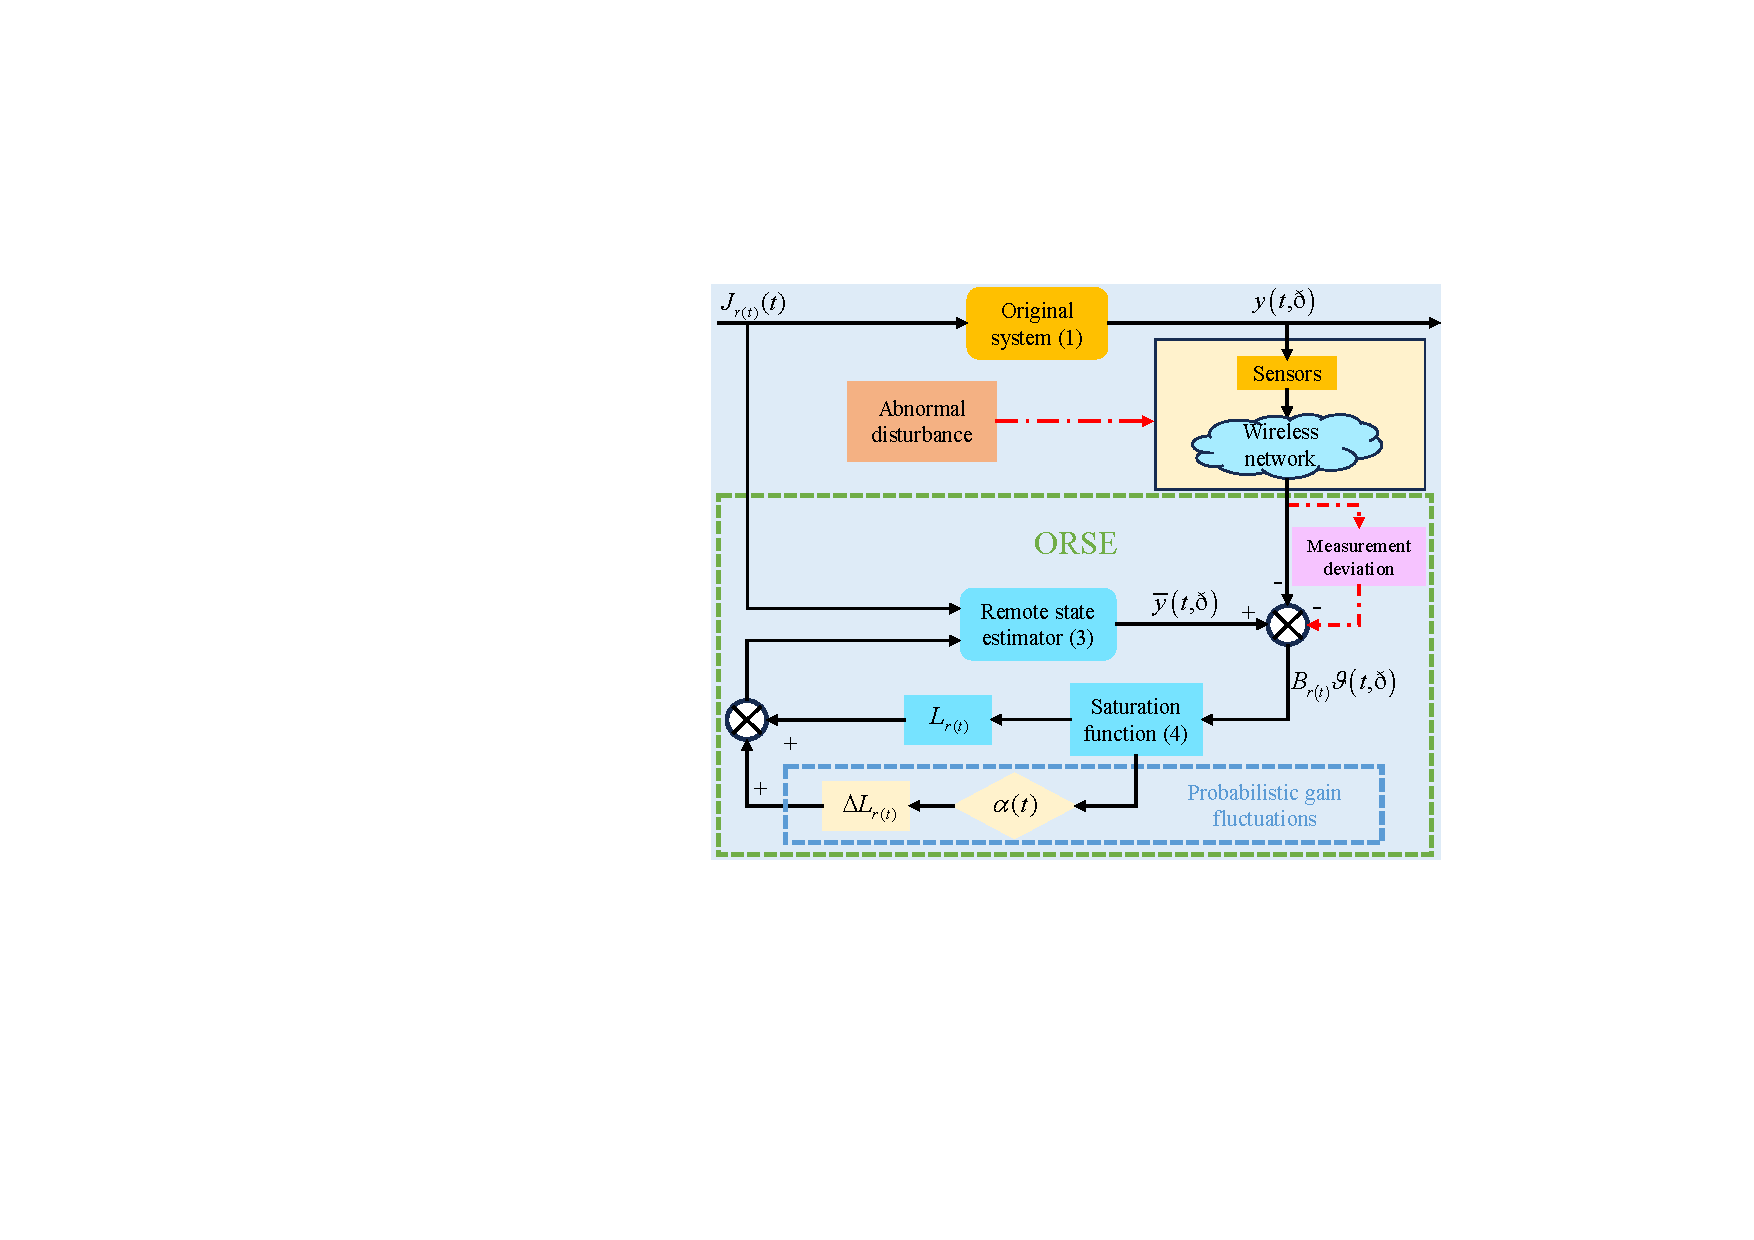
\includegraphics[width=3.5in]{figs/ORSE.pdf} 
		\caption{{\color{red}The framework of the ORSE for semi-Markov switching RDNNs.}} 
		\label{Fig.1} 
	\end{figure}
	Systems \eqref{equ1} and \eqref{equ3} are subject to the following boundary and initial constraints:
	\begin{align}
		\varsigma(t, \eth) = \bar{\varsigma}(t, \eth) = 0,\,(t, \eth) \in [0, +\infty) \times \partial \Omega,
	\end{align}
	\begin{align}
		\varsigma(v, \eth) = \aleph(v, \eth), \, (v, \eth) \in [-\wp, 0] \times \Omega,
	\end{align}
	\begin{align}
		\bar{\varsigma}(v, \eth) = \Im(v, \eth), \, (v, \eth) \in [-\wp, 0] \times \Omega,
	\end{align}
	where $ \aleph(v,\eth), \Im(v ,\eth) \in \mathbb{C}([-\wp, 0] \times \Omega, \mathbb{R}^n) $.

	By  introducing the state error $ \vartheta(t,\eth) = \bar{\varsigma}(t,\eth) - \varsigma(t,\eth) $ and integrating systems \eqref{equ1} and \eqref{equ3}, the corresponding error model is given below:
	\begin{equation}\label{equ9}
		\begin{aligned}
			\frac{\partial \vartheta(t,\eth)}{\partial t} &= \left[ \sum_{k=1}^{q} \frac{\partial}{\partial \eth_k} \left( D_k \frac{\partial \vartheta(t,\eth)}{\partial \eth_k} \right) \right] - A_{r(t)} \vartheta(t,\eth) + W_{1r(t)} g(\vartheta(t,\eth)) + W_{2r(t)} g(\vartheta(t - \wp(t),\eth)) \\ 
			&\quad -G_{r(t)}\omega(t, \eth) + \bar{L}_{r(t)} \phi(B_{r(t)} \vartheta(t,\eth)),\\
		\end{aligned}
	\end{equation}
	where $ g(\vartheta(\cdot, \eth)) = f(\bar{\varsigma}(\cdot, \eth)) - f(\varsigma(\cdot, \eth)) \in \mathbb{R}^n$. To depict the overall research framework more precisely, the schematic diagram of the ORSE for semi-Markov switching RDNNs is displayed in Fig.~\ref{Fig.1}.
	
	Prior to delineating the primary developments, the following indispensable assumption, definition and lemmas should be revisited first.
	\begin{asptn}\label{asptn1}
		For any $ t_1, t_2 \in \mathbb{R}, t_1 \neq t_2 $, activation function $ f_i(\cdot) $ $(i = 1, \dots, n)$ satisfies
		\begin{align*}
			\varkappa_i^{-} \leq \frac{f_i(t_1) - f_i(t_2)}{t_1 - t_2} \leq \varkappa_i^{+},
		\end{align*}
		where $ \varkappa_i^{-}$ and $\varkappa_i^{+} \in \mathbb{R} $.
	\end{asptn}
	
	\begin{Def}\label{Def1}
		The error system \eqref{equ9} is asymptotically stable with an  $\text{H}_\infty$ performance level $\gamma$ if the following criteria are meet:
		
		(1) The error system \eqref{equ9} with $\omega(t,\eth)=0$ is asymptotically stable.
		
		(2) Under zero initial conditions and with $\omega(t,\eth)\neq 0$, the error system \eqref{equ9} is subject to the following inequality.
		\begin{align*}
			\int_{\Omega} \int_{0}^{+\infty} \vartheta^\text{T}(t, \eth) \vartheta(t, \eth) \, dt \, d\eth \leq \gamma^2 \int_{\Omega} \int_{0}^{+\infty} \omega^\text{T}(t, \eth) \omega(t, \eth) \, dt \, d\eth,
		\end{align*}
	where $\gamma$ characterizes the capacity of system to suppress disturbances.
	\end{Def}
	
	\begin{Lem}\label{lem1}
		(\cite{song2021gainscheduled}) For an integral $ \mathcal{N} \geq 0 $, a matrix $\Lambda $ of appropriate dimensions, a real matrix $ H > 0 $, if $ \varphi(t) \in \mathbb{R}^n $ is differentiable over the interval $[p, q]$, then the inequality below is satisfied:
		\begin{align*}
			- \int_p^q \dot{\varphi}^\text{T}(t) H \dot{\varphi}(t) \, dt \leq \epsilon_\mathcal{N}^\text{T} \left( X_\mathcal{N}^\text{T} Y_\mathcal{N}^\text{T} \Lambda + \Lambda^\text{T} Y_\mathcal{N} X_\mathcal{N} + (q - p) \Lambda^\text{T} \mathcal{H}_\mathcal{N}^{-1} \Lambda \right) \epsilon_\mathcal{N},
		\end{align*}
		where
		\begin{align*}
			\epsilon_\mathcal{N} &= \text{col}\left[\varphi(q), \varphi(p), \beta_1, \dots, \beta_\mathcal{N}\right], 
			\mathcal{H}_\mathcal{N} = \text{diag}\left\{H, 3H, \dots, (2\mathcal{N}+1)H\right\},
		\end{align*}
		\begin{align*}
			X_\mathcal{N} &= \begin{bmatrix} 
				I & -I & 0 & 0 & \cdots & 0 \\
				0 & -I & I & 0 & \cdots & 0 \\
				0 & -I & 0 & 2I & \cdots & 0 \\
				\vdots & \vdots & \vdots & \vdots & \ddots & \vdots \\
				0 & -I & 0 & 0 & \cdots & \mathcal{N}I
			\end{bmatrix},
			Y_\mathcal{N} = \begin{bmatrix}
				I & 0 & \cdots & 0 \\
				I & (-1)^1 \binom{1}{1}\binom{1+1}{1}I & \cdots & 0 \\
				\vdots & \vdots & \ddots & \vdots \\
				I & (-1)^1 \binom{\mathcal{N}}{1}\binom{\mathcal{N}+1}{1}I & \cdots & (-1)^\mathcal{N} \binom{\mathcal{N}}{\mathcal{N}} \binom{\mathcal{N}+\mathcal{N}}{\mathcal{N}}I
			\end{bmatrix},
		\end{align*}
		with $\beta_k = \int_p^q \frac{(q - t)^{k-1}}{(q - p)^k} \varphi(t) \, dt \ (k = 1, 2, \dots, \mathcal{N})$.
	\end{Lem}
	\begin{Lem}\label{lem2}
		(\cite{wang2024synchronization}) For an arbitrarily given vector $ \varpi $ of suitable dimensions, any matrices $ X > 0 $ and $ Y > 0 $, there exist an integrable function $ \varphi(t) $ that satisfies
		\begin{align*} 	
			- \int_p^q \varphi^\text{T}(t) X \varphi(t) \, dt \leq \text{Sym} \left\{ \varpi^\text{T} Y \Phi \right\} + (q - p) \varpi^\text{T} Y X^{-1} Y^\text{T} \varpi,
		\end{align*}
		where $ \Phi = \int_p^q \varphi(t) \, dt $.
	\end{Lem}
	\begin{Lem}\label{lem3}
		(\cite{wu2023adaptiveb}) Given $ \varphi(x) \in \mathbb{C}(\Omega,\mathbb{R}^n)$ with the boundary condition $ \varphi(x)\mid_{\partial \Omega} = 0 $, and a matrix $ U >0 $, one obtains:
		\begin{align*}
			\int_\Omega \varphi^\text{T}(x) U \varphi(x) \, ds \leq \left( \frac{\hat{d}_p - \check{d}_p}{\pi} \right)^2 \int_\Omega \left( \frac{\partial \varphi(x)}{\partial x_p} \right)^\text{T} U \left( \frac{\partial \varphi(x)}{\partial x_p} \right) ds,
		\end{align*}
		where $\Omega \triangleq \left\{\check{d}_p \leq x_p \leq \hat{d}_p, \check{d}_p, \hat{d}_p \in \mathbb{R},p=1,2,\cdots,\mathcal{P} \right\}$.
	\end{Lem}
	\begin{Lem}\label{lem4}
		(\cite{li2020dynamic}) For a saturation function $ \phi(\cdot) \in \left[\mathcal{J}_1, \mathcal{J}_2 \right] $, where diagonal matrices $ \mathcal{J}_2 \geq \mathcal{J}_1 \geq 0 $, the inequality below holds:
		\begin{align*}
			\left[\phi(K\vartheta(t, \eth)) - \mathcal{J}_1 K \vartheta(t, \eth)\right]^\text{T} \left[\phi(K\vartheta(t, \eth)) - \mathcal{J}_2 K \vartheta(t, \eth)\right] \leq 0.
		\end{align*}
		The nonlinear function $ \phi(K\vartheta(t, \eth)) $ can be decomposed into linear and nonlinear components:
		\begin{align*}
			\phi(K\vartheta(t, \eth)) = \mathcal{J}_1 K \vartheta(t, \eth) + \psi(K\vartheta(t, \eth)).
		\end{align*}
		Furthermore, the nonlinear part $ \psi(K\vartheta(t, \eth)) \in \Phi $, and $ \Phi $ satisfies
		\begin{align*}
			\Phi \triangleq \{ \psi: \psi^\text{T} (K\vartheta(t, \eth)) \left[\psi(K\vartheta(t, \eth)) - \mathcal{J} K \vartheta(t, \eth)\right] \leq 0 \},\, \mathcal{J} = \mathcal{J}_2 - \mathcal{J}_1.
		\end{align*}
	\end{Lem}

\section{Main Results}\label{sec3}
Several sufficient conditions for establishing the  $\text{H}_\infty$ asymptotic stability of error system \eqref{equ9} are discussed in this section. Before that, the following variables are defined:
\begin{align*}
	\eta(t, \eth) = \text{col}\bigg[ &\vartheta(t, \eth), \vartheta(t - \wp(t), \eth), \vartheta(t - \wp, \eth), g(\vartheta(t, \eth)), \int_{t-\wp}^t \vartheta(\nu, \eth) d\nu, \frac{\partial \vartheta(t, \eth)}{\partial t}, \frac{\partial \vartheta(t - \wp, \eth)}{\partial t},  g(\vartheta(t - \wp(t), \eth)),\\ &\psi(B_u \vartheta(t,\eth)), \zeta(t,\eth), \omega(t,\eth)\bigg],
\end{align*}
\begin{align*}
	\zeta(t, \eth) = \text{col}\left[ \int_{t-\wp}^t \frac{1}{\wp} \vartheta(\nu, \eth) d\nu, \dots, \int_{t-\wp}^t \frac{(t-\nu)^{\mathcal{N}-1}}{\wp^\mathcal{N}} \vartheta(\nu, \eth) d\nu \right],
\end{align*}
\begin{align*}
	\varepsilon_1(t, \eth) = \text{col}\left[ \vartheta(t, \eth), \vartheta(t - \wp, \eth), \int_{t-\wp}^t \vartheta(\nu, \eth) d\nu \right],\, \varepsilon_2(t, \eth) = \text{col}\left[ \vartheta(t, \eth), g(\vartheta(t, \eth)) \right].
\end{align*}
\begin{thm}\label{thm1}
	With given positive scalars  $\mathcal{N}$, $ \wp$, $\bar{\wp}$, $\xi $, the asymptotic stability of the error system \eqref{equ9} with $ \text{H}_{\infty} $ performance bound $\gamma$ holds, provided there exist symmetric matrices $P_u=\begin{bmatrix}
		P_{11u} & P_{12u} & P_{13u} \\
		* & P_{22u} & P_{23u} \\
		* & * & P_{33u}
	\end{bmatrix}$, $R_1$, $Z_1 \textgreater 0$, $Z_2 \textgreater 0$, $T \textgreater 0$, diagonal matrices $\mathcal{K}_1 \textgreater 0$, $\mathcal{K}_2 \textgreater 0$, any matrices  $R_2$, $N$, $\Lambda$, $S$, and the matrix $N$ satisfy $N D_k \textgreater 0$, such that the following conditions hold:
	\begin{align}\label{positive definition}
		\Theta_1 = \begin{bmatrix}
			Z_1 & -Z_1 & 0 \\
			* & Z_1 + R_1 & R_2 \\
			* & * & Z_2
		\end{bmatrix} > 0,
	\end{align}
	\begin{align}
		\Theta_{2u} = \begin{bmatrix}
			\wp^2 Z_1 + \wp P_{11u} & \wp P_{13u} - \wp Z_1 & 0 & \wp P_{12u} \\
			* & Z_1 + R_1 + \wp P_{33u} & R_2 & \wp P_{23u} \\
			* & *& Z_2 & 0 \\
			* & * & * & \wp P_{22u} \\
		\end{bmatrix} > 0,
	\end{align}
	\begin{align}\label{equ12}
		\Xi_u = \begin{bmatrix}
			\Pi_u+\sum_{k=1}^4 \Pi_k & \wp\varrho^\text{T}_3 \Lambda^\text{T} & \wp S & \bar{\alpha}\varrho_6^\text{T} N \mathcal{D}_u & \daleth_u\\
			* & -\mathcal{Z}_\mathcal{N} & 0 & 0 &0 \\
			* & * & -Z_2 & 0 & 0\\
			* & * &* & -\xi I & 0\\
			* & * &* & * & -\xi^{-1} I
		\end{bmatrix} < 0,
	\end{align}
	where
	\begin{align*}
		\rho_\ell = \left[ 0_{p \times (\ell-1)p}, I_p, 0_{p \times (10+\mathcal{N}-\ell)p} \right] \, (\ell = 1, 2, \dots, 10 + \mathcal{N}),
	\end{align*}
	\begin{align*}
		\varrho_1=\text{col}\left[\rho_1,\rho_3,\rho_5\right],\, \varrho_2=\text{col}\left[\rho_6,\rho_7,\rho_1-\rho_3\right],\, \varrho_3=\text{col}\left[\rho_1,\rho_3,\rho_{10},\dots,\rho_{9+\mathcal{N}}\right],
	\end{align*}
	\begin{align*}
		\varrho_4 = \text{col}\left[\rho_1,\rho_4\right],\, \varrho_5=\text{col}\left[\rho_2,\rho_8\right],\, \varrho_6=\rho_1+\rho_6,
	\end{align*}
	\begin{align*}
		\varrho_{7u} &= -N \rho_6 - N A_u \rho_1 + N W_{1u} \rho_4 + N W_{2u} \rho_8 - N G_u \rho_{10+\mathcal{N}} + N L_u \mathcal{J}_1 B_u \rho_1 + N L_u \rho_{9},
	\end{align*}
	\begin{align*}
		\Pi_u &= \varrho_1^\text{T} \sum_{l=1}^{Q} \bar{\lambda}_{ul} P_l \varrho_1 + \text{Sym} \bigg\{\varrho_6^\text{T} \varrho_{7u} + \varrho_2^\text{T} P_u \varrho_2  - \rho_1^\text{T} \sum_{k=1}^{q} \left( \frac{\pi}{\hat{s}_k - \check{s}_k} \right)^2 N D_k \rho_1  - \rho_{9}^\text{T} \rho_{9} + \rho_{9}^\text{T} \mathcal{J} B_u \rho_1 \\&\quad+ \rho_1^\text{T} \frac{M^-+M^+}{2} \mathcal{K}_1 \rho_4 + \rho_2^\text{T} \frac{M^-+M^+}{2} \mathcal{K}_2 \rho_8\bigg\} - \rho_4^\text{T} \mathcal{K}_1 \rho_4 - \rho_1^\text{T} M^- \mathcal{K}_1 M^+ \rho_1  -  \rho_8^\text{T} \mathcal{K}_2 \rho_8 - \rho_2^\text{T} M^- \mathcal{K}_2 M^+ \rho_2, 
	\end{align*}
	\begin{align*}
		\Pi_1 = \rho_1^\text{T} R_1 \rho_1 - \rho_3^\text{T} R_1\rho_3 + \text{Sym}\! \left\{\rho_5^\text{T} R_2 \rho_1 - \rho_3^\text{T} R_2 \rho_5\right\},
	\end{align*}
	\begin{align*}
		\Pi_2 = \wp^2 \rho_6^\text{T} Z_1 \rho_6 + \wp^2 \rho_1^\text{T} Z_2 \rho_1 + \text{Sym}\! \left\{\wp  \varrho_3^\text{T} X_\mathcal{N}^\text{T} Y_\mathcal{N}^\text{T} \Lambda \varrho_3 + \wp S \rho_5 \right\},
	\end{align*}
	\begin{align*}
		\Pi_3 = \varrho_4^\text{T} T \varrho_4-(1-\bar{\wp})\varrho_5^\text{T} T \varrho_5, \, \Pi_4 = \rho_1^\text{T} \rho_1 - \gamma^2 \rho_{10+\mathcal{N}}^\text{T} \rho_{10+\mathcal{N}},
	\end{align*}
	\begin{align*}
		X_\mathcal{N} &= \begin{bmatrix} 
			I & -I & 0 & 0 & \cdots & 0 \\
			0 & -I & I & 0 & \cdots & 0 \\
			0 & -I & 0 & 2I & \cdots & 0 \\
			\vdots & \vdots & \vdots & \vdots & \ddots & \vdots \\
			0 & -I & 0 & 0 & \cdots & \mathcal{N}I
		\end{bmatrix},\quad
		Y_\mathcal{N} = \begin{bmatrix}
			I & 0 & \cdots & 0 \\
			I & (-1)^1 \binom{1}{1}\binom{1+1}{1}I & \cdots & 0 \\
			\vdots & \vdots & \ddots & \vdots \\
			I & (-1)^1 \binom{\mathcal{N}}{1}\binom{\mathcal{N}+1}{1}I & \cdots & (-1)^\mathcal{N} \binom{\mathcal{N}}{\mathcal{N}} \binom{\mathcal{N}+\mathcal{N}}{\mathcal{N}}I
		\end{bmatrix},
	\end{align*}
	\begin{align*}
		\mathcal{Z}_\mathcal{N}&=\text{diag}\left\{Z_1,3Z_1,\dots,(2\mathcal{N}+1)Z_1\right\}, \quad \daleth_u=\left[ \mathcal{M}_u \left( \mathcal{J}_1 B_u \rho_1  + \rho_{9}  \right) \right]^\text{T}.
	\end{align*}
	
	\begin{proof}
		The LKF adopted for the error system \eqref{equ9} is constructed as:
		\begin{align}\label{LKF}
			V(t,\eth)=\sum_{p=1}^{5}V_{p}(t,\eth),
		\end{align}
		where
		\begin{align}\label{V1}
			V_1(t, \eth) = \int_\Omega \varepsilon_1^\text{T}(t, \eth) P_u \varepsilon_1(t, \eth) \, d\eth,
		\end{align}
		\begin{align}\label{V2}
			V_2(t, \eth) = \int_\Omega \int_{t-\wp}^t \vartheta^\text{T}(\nu, \eth) \left[R_1,2R_2\right] \left[ \vartheta^\text{T}(\nu, \eth), \int_\nu^t \vartheta^\text{T}(\mu, \eth) d\mu \right]^\text{T} d\nu \, d\eth,
		\end{align}
		\begin{align}\label{V3}
			V_3(t, \eth) = \wp \int_\Omega \int_{t-\wp}^t \int_\nu^t \left[ \frac{\partial \vartheta^\text{T}(\mu, \eth)}{\partial \mu} Z_1 \frac{\partial \vartheta(\mu, \eth)}{\partial \mu} + \vartheta^\text{T}(\mu, \eth) Z_2 \vartheta(\mu, \eth) \right] d\mu d\nu d\eth,
		\end{align}
		\begin{align}\label{V4}
			V_4(t, \eth) = \int_\Omega \int_{t - \wp(t)}^t \varepsilon_2^\text{T}(\nu, \eth) T \varepsilon_2(\nu, \eth) \, d\nu \, d\eth,
		\end{align}
		\begin{align}\label{V5}
			V_5(t, \eth) = \int_\Omega \sum_{k=1}^{q} \frac{\partial \vartheta^\text{T}(t, \eth)}{\partial \eth_k} N D_k \frac{\partial \vartheta(t, \eth)}{\partial \eth_k} \, d\eth.
		\end{align}
		
		By Jensen inequality \cite{zhang2022quasisynchronization}, we have
		\begin{align}\label{equ19}
			\wp \int_\nu^t \frac{\partial \vartheta^\text{T}(\mu, \eth)}{\partial \mu} Z_1 \frac{\partial \vartheta(\mu, \eth)}{\partial \mu} d\mu \geq (\vartheta(t, \eth) - \vartheta(\nu, \eth))^\text{T} Z_1 (\vartheta(t, \eth) - \vartheta(\nu, \eth)),
		\end{align}
		\begin{align}\label{equ20}
			\wp \int_\nu^t \vartheta^\text{T}(\mu, \eth) Z_2 \vartheta(\mu, \eth) d\mu \geq \int_\nu^t \vartheta^\text{T}(\mu, \eth) d\mu Z_2 \int_\nu^t \vartheta(\mu, \eth) d\mu. 
		\end{align}
		
		According to \eqref{equ19} and \eqref{equ20}, we can deduce
		\begin{align} 
			V_2(t, \eth) + V_3(t, \eth) &\geq \int_\Omega \int_{t - \wp}^t (\vartheta(t, \eth) - \vartheta(\nu, \eth))^\text{T} Z_1 (\vartheta(t, \eth) - \vartheta(\nu, \eth)) \, d\nu \, d\eth\nonumber\\
			&\quad + \int_\Omega \int_{t-\wp}^t \left[ \int_\nu^t \vartheta^\text{T}(\mu, \eth) d\mu Z_2 \int_\nu^t \vartheta(\mu, \eth) d\mu \right] d\nu \, d\eth\nonumber\\
			&\quad + \int_\Omega \int_{t-\wp}^t \begin{bmatrix} \vartheta(\nu,\eth) \\ \int_\nu^t \vartheta(\nu, \eth) d\mu \end{bmatrix} ^\text{T} \begin{bmatrix} R_1 & R_2 \\ * & 0 \end{bmatrix} \begin{bmatrix} \vartheta(\nu,\eth) \\ \int_\nu^t \vartheta(\nu, \eth) d\mu \end{bmatrix} d\nu \, d\eth\nonumber\\
			&= \int_\Omega \int_{t-\wp}^t \left[ \begin{array}{c} \vartheta(t, \eth) \\ \vartheta(\nu, \eth)\\\int_\nu^t \vartheta(\mu, \eth) d\mu \end{array} \right]^\text{T} \Theta_1 \left[ \begin{array}{c} \vartheta(t, \eth) \\ \vartheta(\nu, \eth)\\\int_\nu^t \vartheta(\mu, \eth) d\mu \end{array} \right] d\nu \, d\eth,
		\end{align}
		where $\Theta_1 = \begin{bmatrix}
			Z_1 & -Z_1 & 0 \\
			* & Z_1 + R_1 & R_2 \\
			* & * & Z_2
		\end{bmatrix} $.
		
		Then, we can infer
		\begin{align}
			\sum_{p=1}^3 V_p(t, \eth) 
			&\geq V_1(t, \eth) + \int_\Omega \int_{t-\wp}^t \left[ \begin{array}{c} \vartheta(t, \eth) \\ \vartheta(\nu, \eth)\\\int_\nu^t \vartheta(\mu, \eth) d\mu \end{array} \right]^\text{T} \Theta_1 \left[ \begin{array}{c} \vartheta(t, \eth) \\ \vartheta(\nu, \eth)\\\int_\nu^t \vartheta(\mu, \eth) d\mu \end{array} \right] d\nu \, d\eth\nonumber\\
			&\geq \frac{1}{\wp} \int_\Omega \left[ \begin{array}{c} \vartheta(t, \eth) \\ \int_{t-\wp}^t \vartheta(\nu, \eth) d\nu\\\int_{t-\wp}^t \int_\nu^t \vartheta(\mu, \eth) d\mu d\nu \\ \vartheta(t-\wp,\eth)\end{array} \right]^\text{T} \Theta_{2u} \left[ \begin{array}{c} \vartheta(t, \eth) \\ \int_{t-\wp}^t \vartheta(\nu, \eth) d\nu\\\int_{t-\wp}^t \int_\nu^t \vartheta(\mu, \eth) d\mu d\nu \\ \vartheta(t-\wp,\eth)\end{array} \right] d\eth > 0,
		\end{align}
		where $\Theta_{2u} = \begin{bmatrix}
			\wp^2 Z_1 + \wp P_{11u} & \wp P_{13u} - \wp Z_1 & 0 & \wp P_{12u} \\
			* & Z_1 + R_1 + \wp P_{33u} & R_2 & \wp P_{23u} \\
			* & * & Z_2 & 0 \\
			* & * & * & \wp P_{22u}
		\end{bmatrix}$.
		
		According to $\Theta_{1}\textgreater 0$, $\Theta_{2u} \textgreater 0 $, $ T \textgreater 0 $, $ N D_k \textgreater 0 $, clearly, $ V(t, \eth)$ is positive definite. Subsequently, its weak infinitesimal operator is given by:
		\begin{align}\label{DLKF}
			\mathcal{L}V(t,\eth)=\sum_{p=1}^{5}\mathcal{L}V_{p}(t,\eth).
		\end{align}
		
		The expectation of the weak infinitesimal operator of the mode-dependent LKF:
		\begin{align}\label{equ24}
			\mathbb{E} \{ \mathcal{L} V_1(t, \eth) \} &= \int_\Omega \left[ \sum_{l=1}^{Q} \bar{\lambda}_{ul} \varepsilon_1^\text{T}(t, \eth) P_l \varepsilon_1(t, \eth) + 2 \frac{\partial \varepsilon_1^\text{T}(t, \eth)}{\partial t} P_u \frac{\partial \varepsilon_1(t, \eth)}{\partial t} \right] d\eth\nonumber\\
			&= \int_\Omega \eta^\text{T}(t, \eth) \left[ \varrho_1^\text{T} \sum_{l=1}^Q \bar{\lambda}_{ul} P_l \varrho_1 + 2 \varrho_2^\text{T} P_u \varrho_2 \right] \eta(t, \eth) \, d\eth,
		\end{align}
		where $\bar{\lambda}_{ul} = \mathbb{E} \{ \lambda_{ul}(\hbar) \} = \int_0^\infty \lambda_{ul}(\hbar) \mathcal{F}_u(\hbar) \, d\hbar$, and $\mathcal{F}_u(\hbar)$ is the probability density function (PDF) of ST $\hbar$ associated with mode $u$.
		\begin{align}\label{equ25}
			\mathbb{E} \{ \mathcal{L} V_2(t, \eth) \} &= \int_\Omega \left[ \vartheta^\text{T}(t, \eth) R_1 \vartheta(t, \eth) + 2\int_{t-\wp}^t \vartheta^\text{T}(\nu, \eth) d\nu R_2 \vartheta(t, \eth) \right.\nonumber\\
			&\quad \left.- \vartheta^\text{T}(t - \wp, \eth) R_1 \vartheta(t - \wp, \eth) - 2\vartheta^\text{T}(t - \wp, \eth) R_2 \int_{t-\wp}^t \vartheta(\nu, \eth) d\nu \,\right] d\eth \nonumber\\
			&= \int_\Omega \eta^\text{T}(t, \eth) \left[ \rho_1^\text{T} R_1 \rho_1 + 2\rho_5^\text{T} R_2 \rho_1 - \rho_3^\text{T} R_1 \rho_3 - 2\rho_3^\text{T} R_2 \rho_5 \right] \eta(t, \eth) \, d\eth,
		\end{align}
		\begin{align}\label{dv3}
			\mathbb{E} \{ \mathcal{L} V_3(t, \eth) \} &= \int_\Omega \left[ \wp^2 \frac{\partial \vartheta^\text{T}(t, \eth)}{\partial t} Z_1 \frac{\partial \vartheta(t, \eth)}{\partial t} + \wp^2 \vartheta^\text{T}(t, \eth) Z_2 \vartheta(t, \eth)\right.\nonumber\\
			&\quad \left.- \wp \int_{t-\wp}^t \left( \frac{\partial \vartheta^\text{T}(\nu, \eth)}{\partial \nu} Z_1 \frac{\partial \vartheta(\nu, \eth)}{\partial \nu} + \vartheta^\text{T}(\nu, \eth) Z_2 \vartheta(\nu, \eth) \right) d\nu \,\right] d\eth. 
		\end{align}
		
		By applying Lemmas \ref{lem1} and \ref{lem2}, the inequalities below can be derived:
		\begin{align}\label{equ27}
			- \wp \int_{t-\wp}^t \frac{\partial \vartheta^\text{T}(\nu, \eth)}{\partial \nu} Z_1 \frac{\partial \vartheta(\nu, \eth)}{\partial \nu} d\nu \leq \wp \beth_\mathcal{N}^\text{T} \left( X_\mathcal{N}^\text{T} Y_\mathcal{N}^\text{T} \Lambda + \Lambda^\text{T} Y_\mathcal{N} X_\mathcal{N} + \wp \Lambda^\text{T} \mathcal{Z}_\mathcal{N}^{-1} \Lambda\right) \beth_\mathcal{N},
		\end{align}
		\begin{align}\label{equ28}
			- \wp \int_{t-\wp}^t \vartheta^\text{T}(\nu, \eth) Z_2 \vartheta(\nu, \eth) d\nu \leq \text{Sym} \left\{ \wp\eta^\text{T}(t, \eth)  S \int_{t-\wp}^t \vartheta(\nu, \eth) d\nu \right\}+ \wp^2\eta^\text{T}(t, \eth)  S Z_2^{-1} S^\text{T} \eta(t,\eth),
		\end{align}
		where $\beth_\mathcal{N} = \text{col} \left[\vartheta(t, \eth), \vartheta(t - \wp, \eth), \int_{t - \wp}^t \frac{1}{\wp} \vartheta(\nu, \eth) d\nu, \dots, \int_{t - \wp}^t \frac{(t - \nu)^{\mathcal{N} - 1}}{\wp^\mathcal{N}} \vartheta(\nu, \eth) d\nu \right]$.
		
		Therefore, from \eqref{equ27} and \eqref{equ28}, it follows that
		
		\begin{align}\label{equ29}
			\mathbb{E}\left\{ \mathcal{L}V_3(t, \eth) \right\} &\leq \int_\Omega \bigg[ \wp^2 \frac{\partial \vartheta^\text{T}(t, \eth)}{\partial t} Z_1 \frac{\partial \vartheta(t, \eth)}{\partial t} + \wp \beth_\mathcal{N}^\text{T} \left( X_\mathcal{N}^\text{T} Y_\mathcal{N}^\text{T} \Lambda + A^\text{T} Y_\mathcal{N} X_\mathcal{N} + \wp \Lambda^\text{T} \mathcal{Z}_\mathcal{N}^{-1} \Lambda \right) \beth_\mathcal{N} \nonumber\\ & \quad 
			+ \wp^2 \vartheta^\text{T}(t, \eth) Z_2 \vartheta(t, \eth) + \text{Sym} \left\{ \wp \eta^\text{T}(t, \eth)  S \int_{t-\wp}^t \vartheta(\nu, \eth) d\nu \right\} + \wp^2 \eta^\text{T}(t, \eth) S Z_2^{-1} S^\text{T} \eta(t, \eth)\bigg] d\eth \nonumber\\
			&= \int_\Omega \eta^\text{T}(t, \eth) \left[ \wp^2 \rho_6^\text{T}  Z_1 \rho_6 + \wp^2 \rho_1^\text{T}  Z_2 \rho_1 + \wp \varrho_3^\text{T}  \left( \text{Sym} \left\{ X_\mathcal{N}^\text{T} Y_\mathcal{N}^\text{T} \Lambda \right\} + \wp \Lambda^\text{T} \mathcal{Z}_\mathcal{N}^{-1} \Lambda \right) \varrho_3 \right.\nonumber\\ & \quad \left.+ \text{Sym} \left\{ \wp S \rho_5 \right\} + \wp^2 S Z_2^{-1} S^\text{T}\right] \eta(t, \eth) d\eth,
		\end{align}
		\begin{align}
			\mathbb{E}\{\mathcal{L} V_4(t, \eth)\} &= \int_\Omega \left[ \varepsilon_2^\text{T}(t, \eth) T \varepsilon_2(t, \eth) - (1 - \dot{\wp}(t)) \varepsilon_2^\text{T}(t - \wp(t), \eth) T \varepsilon_2(t - \wp(t), \eth) \right] d\eth \nonumber\\
			& \leq \int_\Omega \eta^\text{T}(t, \eth) \left[ \varrho_4^\text{T} T \varrho_4 - (1 - \bar{\wp}) \varrho_5^\text{T} T \varrho_5 \right] \eta(t, \eth) d\eth,
		\end{align}
		\begin{align}
			\mathbb{E}\left\{\mathcal{L} V_5(t, \eth)\right\} = 2 \int_\Omega \sum_{k=1}^q \frac{\partial^2 \vartheta^\text{T}(t, \eth)}{\partial \eth_k \partial t} N D_k \frac{\partial \vartheta(t, \eth)}{\partial \eth_k} d\eth.
		\end{align}
		
		The following equation is derived by applying the free-weighting matrix approach:
		\begin{align}\label{equ32}
			0&=2\int_\Omega\left[\vartheta^\text{T}(t,\eth)+\frac{\partial \vartheta^\text{T}(t,\eth)}{\partial t}\right]N\bigg[-\frac{\partial \vartheta(t,\eth)}{\partial t}+ \left(\sum_{k=1}^{q} \frac{\partial}{\partial \eth_k} \left( D_k \frac{\partial \vartheta(t,\eth)}{\partial \eth_k} \right) \right) - A_u \vartheta(t,\eth) + W_{1u} g(\vartheta(t,\eth))\nonumber\\ 
			&\quad + W_{2u} g(\vartheta(t - \wp(t),\eth)) -G_u \omega(t, \eth) + \bar{L}_u \phi(B_u \vartheta(t,\eth)) \bigg] d\eth.
		\end{align}
		
		Further, in view of Lemma \ref{lem3} and the boundary condition, we obtain
		\begin{align}\label{equ33}
			2 &\int_\Omega \vartheta^\text{T}(t, \eth) N \sum_{k=1}^q \frac{\partial}{\partial \eth_k} \left( D_k \frac{\partial \vartheta(t, \eth)}{\partial \eth_k} \right) d\eth\nonumber\\
			&= 2 \sum_{k=1}^q \vartheta^\text{T}(t, \eth) N D_k \frac{\partial \vartheta(t, \eth)}{\partial \eth_k} \Bigg|_{\partial \Omega} - 2 \int_\Omega \sum_{k=1}^q \frac{\partial \vartheta^\text{T}(t,\eth)}{\partial \eth_k} N D_k \frac{\partial \vartheta(t, \eth)}{\partial \eth_k} d\eth\nonumber\\
			&= -2 \int_\Omega \sum_{k=1}^q \frac{\partial \vartheta^\text{T}(t, \eth)}{\partial \eth_k} N D_k \frac{\partial \vartheta(t, \eth)}{\partial \eth_k} d\eth\nonumber\\
			&\leq -2 \int_\Omega \vartheta^\text{T}(t, \eth) \sum_{k=1}^q \left( \frac{\pi}{\hat{s}_k - \check{s}_k} \right)^2 N D_k \vartheta(t, \eth) d\eth.
		\end{align}
		
		Furthermore, the application of Green formula and the boundary conditions yields:
		\begin{align}\label{equ34}
			2 &\int_\Omega \frac{\partial \vartheta^\text{T}(t, \eth)}{\partial t} N \sum_{k=1}^q \frac{\partial}{\partial \eth_k} \left( D_k \frac{\partial \vartheta(t, \eth)}{\partial \eth_k} \right) d\eth\nonumber\\
			&= 2 \sum_{k=1}^q \frac{\partial \vartheta^\text{T}(t, \eth)}{\partial t} N D_k \frac{\partial \vartheta(t, \eth)}{\partial \eth_k} \Bigg|_{\partial \Omega} - 2 \int_\Omega \sum_{k=1}^q \frac{\partial^2 \vartheta^\text{T}(t, \eth)}{\partial \eth_k \partial t} N D_k \frac{\partial \vartheta(t, \eth)}{\partial \eth_k} d\eth \nonumber\\
			&= -2 \int_\Omega \sum_{k=1}^q \frac{\partial^2 \vartheta^\text{T}(t, \eth)}{\partial \eth_k \partial t} N D_k \frac{\partial \vartheta(t, \eth)}{\partial \eth_k} d\eth.
		\end{align}
		
		From Lemma \ref{lem4}, the saturation function term in equation \eqref{equ9} satisfy
		\begin{align}
			\phi(B_u \vartheta(t, \eth)) = \mathcal{J}_1 B_u \vartheta(t, \eth) + \psi(B_u \vartheta(t, \eth)),
		\end{align}
		and
		\begin{align}
			- 2\psi^\text{T} (B_u \vartheta(t, \eth)) \left[ \psi(B_u \vartheta(t, \eth)) - \mathcal{J} B_u \vartheta(t, \eth) \right] \geq 0.
		\end{align}
		
		Assumption \ref{asptn1} ensures the existence of diagonal matrices $\mathcal{K}_i \textgreater 0 \,(i=1,2)$ for which the inequalities below are valid:
		\begin{align}
			\int_{\Omega} &\left[ g(\vartheta(t,\eth)) - M^- \vartheta(t,\eth) \right]^\text{T} \mathcal{K}_1 \left[ M^+ \vartheta(t,\eth) - g(\vartheta(t,\eth)) \right] d\eth \geq 0,
		\end{align}
		\begin{align}\label{equ38}
			\int_{\Omega} &\left[ g(\vartheta(t-\wp(t),\eth)) - M^- \vartheta(t-\wp(t),\eth) \right]^\text{T} \mathcal{K}_2 \left[ M^+ \vartheta(t-\wp(t),\eth) - g(\vartheta(t-\wp(t),\eth)) \right] d\eth \geq 0,
		\end{align}
		where $M^-=\text{diag}\left\{\varkappa_1^-,\varkappa_2^-,\dots,\varkappa_n^-\right\}$ and $M^+=\text{diag}\left\{\varkappa_1^+,\varkappa_2^+,\dots,\varkappa_n^+\right\}$.
		
		According to $\mathbb{E}\{\alpha(t)\}=\bar{\alpha}$, combining \eqref{equ24}, \eqref{equ25}, and \eqref{equ29}-\eqref{equ38}, it yield
		\begin{align}\label{equ39}
			\mathbb{E}\{ \mathcal{L} V(t, \eth) \} \leq \mathbb{E} \left\{ \int_{\Omega} \left[ \eta^\text{T}(t,\eth) \Upsilon \eta(t,\eth) - \vartheta^\text{T}(t, \eth) \vartheta(t, \eth) + \gamma^2 \omega^\text{T}(t, \eth) \omega(t, \eth) \right] d\eth \right\},
		\end{align}
		where $\Upsilon = \Pi_u+\sum_{k=1}^4 \Pi_k + \wp^2 \varrho_3^\text{T} \Lambda^\text{T} \mathcal{Z}_\mathcal{N}^{-1} \Lambda \varrho_3 + \wp^2 S Z_2^{-1} S^\text{T} + \text{Sym} \left\{ \bar{\alpha}\varrho_6^\text{T} N  \Delta L_u \left( \mathcal{J}_1 B_u \rho_1  + \rho_9 \right) \right\}$ with $\Delta L_u =\mathcal{D}_u F_u \mathcal{M}_u$.
		
		Based on inequality $\text{Sym} \{ \mathcal{W}_1 \mathcal{W}_2 \} \leq \xi^{-1} \mathcal{W}_1 \mathcal{W}_1^\text{T} + \xi \mathcal{W}_2^\text{T} \mathcal{W}_2$ in \cite{tai2023asynchronous}, we can infer
		\begin{align}
			\text{Sym} \left\{ \bar{\alpha}\varrho_6^\text{T} N \mathcal{D}_u F_u \mathcal{M}_u \left( \mathcal{J}_1 B_u \rho_1 + \rho_9  \right) \right\}
			\leq \xi^{-1} \left( \bar{\alpha}\varrho_6^\text{T} N \mathcal{D}_u \right) \left( \bar{\alpha}\varrho_6^\text{T} N \mathcal{D}_u \right)^\text{T} + \xi \daleth_u \daleth_u^\text{T},
		\end{align}
		where $\daleth_u=\left[\mathcal{M}_u \left( \mathcal{J}_1 B_u \rho_1  + \rho_9 \right)\right]^\text{T}$.
		
		According to Schur complement, $\Upsilon  \textless 0$ is equal to the inequality \eqref{equ12}. Thus, inequality \eqref{equ39} can be derived as follows:
		\begin{align}
			\mathbb{E}\{ \mathcal{L} V(t, \eth) \} \leq  \int_{\Omega}  \left[- \vartheta^\text{T}(t, \eth) \vartheta(t, \eth) + \gamma^2 \omega^\text{T}(t, \eth) \omega(t, \eth)\right] d\eth.
		\end{align}
		
		\textbf{Case \uppercase\expandafter{\romannumeral1} :} When $\omega(t,\eth) = 0$, it follows that:
		\begin{align}
			\mathbb{E} \left\{ \mathcal{L} V(t, \eth) \right\} \leq \int_{\Omega} -\vartheta^\text{T}(t, \eth) \vartheta(t, \eth) \, d\eth \leq -\| \vartheta(t, \eth) \| \leq 0.
		\end{align}
		
		Thus, the error system \eqref{equ9} is asymptotic stability.
		
		\textbf{Case \uppercase\expandafter{\romannumeral2} :} When $\omega(t,\eth) \neq 0$, one can obtain:
		\begin{align}
			V(+\infty, \eth) - V(0, \eth) \leq \int_{\Omega} \int_{0}^{+\infty} \left[-\vartheta^\text{T}(t, \eth) \vartheta(t, \eth) + \gamma^2 \omega^\text{T}(t, \eth) \omega(t, \eth)\right] \, dt \, d\eth.
		\end{align}
		
		Given the zero initial state and the fact that $V(+\infty, \eth) \textgreater 0$, the following conclusion can be drawn:
		\begin{align}
			\int_{\Omega} \int_{0}^{+\infty} \vartheta^\text{T}(t, \eth) \vartheta(t, \eth) \, dt \, d\eth \leq \gamma^2 \int_{\Omega} \int_{0}^{+\infty} \omega^\text{T}(t, \eth) \omega(t, \eth) \, dt \, d\eth.
		\end{align}
		
		Therefore, the error system \eqref{equ9} satisfies $\text{H}_\infty$ performance. The proof is thus finished.
	\end{proof}
	
	\begin{rem}\label{rem5}
		It is noteworthy that an important characteristic of $V_1(t, \eth)$ is its dependence on the system mode. In addition, unlike conventional LKFs, the constructed $V_2(t, \eth)$ is asymmetric. However, when $R_2 = 0$ in Theorem \ref{thm1}, $V_2(t, \eth)$ degenerates into a symmetric form. Moreover, the positive definiteness condition of this LKF is more relaxed compared to traditional LKF, requiring only the matrices $\Theta_{1}$, $\Theta_{2u}$, $T$ and $N D_k$ to be positive definite, without imposing positive definiteness on all related matrices, thereby reducing the conservatism in the analysis process. {\color{red}Furthermore, for the $u$th semi-Markov mode in Theorem \ref{thm1}, the number of decision variables is $n[8.5n+0.5(\mathcal{N}+1)( \mathcal{N}+2)n+(\mathcal{N}+10)n+5.5]$. It is worth noting that if $V_2(t, \eth)$ were replaced by a general symmetric augmented LKF of the form $V_2(t, \eth) = \int_\Omega \int_{t-\wp}^t \left[\vartheta^\text{T}(\nu, \eth), \int_\nu^t \vartheta^\text{T}(\mu, \eth) d\mu \right] R \left[ \vartheta^\text{T}(\nu, \eth), \int_\nu^t \vartheta^\text{T}(\mu, \eth) d\mu \right]^\text{T} d\nu \, d\eth$, where $R \in \mathbb{R}^{2n \times 2n}$ is positive define matrix, the resulting $V_2(t, \eth)$ would significantly increase the complexity of condition \eqref{equ12}, thereby raising the computational complexity.}
	\end{rem}
	\begin{rem}\label{rem6}
		 It is worth highlighting that equation (32), introduced via the free-weighting matrix technique, includes the reaction-diffusion terms $2 \int_\Omega \vartheta^\text{T}(t, \eth) N \sum_{k=1}^q \frac{\partial}{\partial \eth_k} \left( D_k \frac{\partial \vartheta(t, \eth)}{\partial \eth_k} \right) d\eth$ and $2\int_\Omega \frac{\partial \vartheta^\text{T}(t, \eth)}{\partial t} N \sum_{k=1}^q \frac{\partial}{\partial \eth_k} \left( D_k \frac{\partial \vartheta(t, \eth)}{\partial \eth_k} \right) d\eth$, which complicate the subsequent analysis. To address this problem, Lemma \ref{lem3}, Green formula and the system boundary conditions are employed to transform reaction-diffusion terms in \eqref{equ32} into equation \eqref{equ33} and \eqref{equ34}. Moreover, a specifically constructed LKF $V_5(t,\eth)$ ensures that $\mathbb{E}\left\{\mathcal{L} V_5(t, \eth)\right\}$ cancels with equation \eqref{equ34}, thereby eliminating the reaction-diffusion terms.
	\end{rem}
\end{thm}

Evidently, due to the presence of coupling terms in Theorem \ref{thm1}, the estimator gain cannot be directly determined. To circumvent this issue, Theorem \ref{thm2} proffers a design strategy for the estimator gain.
\begin{thm}\label{thm2}
		With given positive scalars  $\mathcal{N}$, $ \wp$, $\bar{\wp}$, $\xi $, the asymptotic stability of the error system \eqref{equ9} with $ \text{H}_{\infty} $ performance bound $\gamma$ holds, provided there exist symmetric matrices $P_u=\begin{bmatrix}
		P_{11u} & P_{12u} & P_{13u} \\
		* & P_{22u} & P_{23u} \\
		* & * & P_{33u}
	\end{bmatrix}$, $R_1$, $Z_1 \textgreater 0$, $Z_2 \textgreater 0$, $T \textgreater 0 $, diagonal matrices $\mathcal{K}_1 \textgreater 0$, $\mathcal{K}_2 \textgreater 0$, any matrices  $R_2$, $N$, $\Lambda$, $S$, and the matrix $N$ satisfy $N D_k \textgreater 0$, such that the following linearization conditions hold:
	\begin{align}\label{equ45}
		\Theta_1 = \begin{bmatrix}
			Z_1 & -Z_1 & 0 \\
			* & Z_1 + R_1 &  R_2 \\
			* & * & Z_2
		\end{bmatrix} > 0,
	\end{align}
	\begin{align}\label{equ46}
		\Theta_{2u} = \begin{bmatrix}
			\wp^2 Z_1 + \wp P_{11u} & \wp P_{13u} - \wp Z_1 & 0 & \wp P_{12u} \\
			* & Z_1 + R_1 + \wp P_{33u} & R_2 & \wp P_{23u} \\
			* & *& Z_2 & 0 \\
			* & * & * & \wp P_{22u} \\
		\end{bmatrix} > 0,
	\end{align}
	\begin{align}\label{equ47}
		\hat{\Xi}_u = \begin{bmatrix}
			\hat{\Pi}_u+\sum_{k=1}^4 \Pi_k & \wp\varrho^\text{T}_3 \Lambda^\text{T} & \wp S & \bar{\alpha}\varrho_6^\text{T} N \mathcal{D}_u & \daleth_u\\
			* & -\mathcal{Z}_\mathcal{N} & 0 & 0 &0 \\
			* & * & -Z_2 & 0 & 0\\
			* & * &* & -\xi I & 0\\
			* & * &* & * & -\xi^{-1} I
		\end{bmatrix} < 0,
	\end{align}
	where
	\begin{align*}
		\hat{\Pi}_u&=\Pi_u - \text{Sym} \{\varrho_6^\text{T} \varrho_{7u} \} + \text{Sym} \{\varrho_6^\text{T} \hat{\varrho}_{7u} \}, 
	\end{align*}
	\begin{align*}
		\hat{\varrho}_{7u} &=-N \rho_6 - N A_u \rho_1 + N W_{1u} \rho_4 + N W_{2u} \rho_8 - N G_u \rho_{10+\mathcal{N}} + \hat{L}_u \mathcal{J}_1 B_u \rho_1 + \hat{L}_u \rho_9.
	\end{align*}
	
	Furthermore, all other parameters follow the definition given in Theorem \ref{thm1}, and the estimator gains can be acquired by exploiting the relationships
	\begin{align}
		L_u=N^{-1}\hat{L}_u.
	\end{align}
	\begin{proof}
		Defining $\hat{L}_u=NL_u$, the expression \eqref{equ39} becomes
		\begin{align}
			\mathbb{E}\{ \mathcal{L} V(t, \eth) \} \leq \mathbb{E} \left\{ \int_{\Omega} \left[ \eta^\text{T}(t, \eth) \hat{\Upsilon} \eta(t,\eth) - \vartheta^\text{T}(t, \eth) \vartheta(t, \eth) + \gamma^2 \omega^\text{T}(t, \eth) \omega(t, \eth) \right] d\eth \right\},
		\end{align}
		where $\hat{\Upsilon}=\hat{\Pi}_u+\sum_{k=1}^4 \Pi_k+\wp^2\varrho^\text{T}_3 \Lambda^\text{T}\mathcal{Z}^{-1}_\mathcal{N}\Lambda\varrho_3+\wp^2 S Z^{-1}_2 S^\text{T}+ \xi^{-1} \left( \bar{\alpha}\varrho_6^\text{T} N \mathcal{D}_u \right) \left( \bar{\alpha}\varrho_6^\text{T} N \mathcal{D}_u \right)^\text{T} + \xi \daleth_u \daleth_u^\text{T}$.
		
		According to Schur complement, $\hat{\Upsilon} \textless 0$  is equal to linear matrix inequality (LMI) \eqref{equ47}. The proof that follows resembles that of Theorem \ref{thm1}, and the proof is thus completed.
	\end{proof}
\end{thm}

When the saturation function in ORSE \eqref{equ3} is removed, the estimator degenerates into a conventional resilient state estimator. Under this scenario, the estimation error system implies that

\begin{cor}\label{cor1}
		With given positive scalars  $\mathcal{N}$, $ \wp$ $\bar{\wp}$, $\xi $, the asymptotic stability of the error system \eqref{equ9} with $ \text{H}_{\infty} $ performance bound $\gamma$ holds, provided there exist symmetric matrices $P_u=\begin{bmatrix}
		P_{11u} & P_{12u} & P_{13u} \\
		* & P_{22u} & P_{23u} \\
		* & * & P_{33u}
	\end{bmatrix}$, $R_1$, $Z_1 \textgreater 0$, $Z_2 \textgreater 0$, $T \textgreater 0 $, diagonal matrices $\mathcal{K}_1 \textgreater 0$, $\mathcal{K}_2 \textgreater 0$, any matrices  $R_2$, $N$, $\Lambda$, $S$, and the matrice $N$ satisfy $N D_k \textgreater 0$, such that the following linearization conditions hold:
	\begin{align}\label{equ50}
		\Theta_1 = \begin{bmatrix}
			Z_1 & -Z_1 & 0 \\
			* & Z_1 + R_1 & R_2 \\
			* & * & Z_2
		\end{bmatrix} > 0,
	\end{align}
	\begin{align}\label{equ51}
		\Theta_{2u} = \begin{bmatrix}
			\wp^2 Z_1 + \wp P_{11u} & \wp P_{13u} - \wp Z_1 & 0 & \wp P_{12u} \\
			* & Z_1 + R_1 + \wp P_{33u} & R_2 & \wp P_{23u} \\
			* & *& Z_2 & 0 \\
			* & * & * & \wp P_{22u} \\
		\end{bmatrix} > 0,
	\end{align}
	\begin{align}\label{equ52}
		\tilde{\Xi}_u = \begin{bmatrix}
			\tilde{\Pi}_u+\sum_{k=1}^4 \Pi_k & \wp\varrho^\text{T}_3 \Lambda^\text{T} & \wp S & \bar{\alpha}\varrho_6^\text{T} N \mathcal{D}_u & \tilde{\daleth}_u\\
			* & -\mathcal{Z}_\mathcal{N} & 0 & 0 &0 \\
			* & * & -Z_2 & 0 & 0\\
			* & * &* & -\xi I & 0\\
			* & * &* & * & -\xi^{-1} I
		\end{bmatrix} < 0,
	\end{align}
	where
	\begin{align*}
		\tilde{\Pi}_u&=\hat{\Pi}_u - \text{Sym} \{\varrho_6^\text{T} \hat{\varrho}_{7u} - \rho_{9}^\text{T} \rho_{9} + \rho_{9}^\text{T} \mathcal{J}_1 B_u \rho_1 \} + \text{Sym} \{\varrho_6^\text{T} \tilde{\varrho}_{7u} \},
	\end{align*}
	\begin{align*}
		\tilde{\varrho}_{7u} &=-N \rho_6 - N A_u \rho_1 + N W_{1u} \rho_4 + N W_{2u} \rho_8 - N G_u \rho_{10+\mathcal{N}} + \hat{L}_u B_u \rho_1,\, \tilde{\daleth}_u= \rho_1 ^\text{T} B_u^\text{T} \mathcal{M}_u^\text{T}.
	\end{align*}
	
	The other parameters in the LMIs \eqref{equ50}-\eqref{equ52} which not listed can be found in Theorem \ref{thm2}, and the gains can be obtained by $L_u=N^{-1}\hat{L}_u$.
\end{cor}

\begin{rem}\label{rem7}
	Within the framework of $\text{H}_\infty$ asymptotic stability, Theorem \ref{thm1} provides sufficient conditions under which the ORSE can be guaranteed to exist. Based on Theorem \ref{thm1}, Theorem \ref{thm2} further provides a method for solving the estimator gain in the presence of measurement outliers. In contrast to Theorem \ref{thm2}, Corollary \ref{cor1} offers an alternative design by deriving the existence conditions and gain calculation method for the resilient state estimator. Compared with existing designs of outlier-resilient estimators, this work introduces an asymmetric LKF to derive key results, especially under network parameter variations and reaction–diffusion dynamic.
\end{rem}
\begin{rem}\label{rem8}
	{\color{red}The lower value of $\gamma$ indicates better capability in suppressing external disturbances and maintaining system stability. Therefore, minimizing the $\text{H}_\infty$ performance index $\gamma$ is crucial in practical systems. Based on the results in Theorem \ref{thm2}, the optimization problem for minimizing the $\text{H}_\infty$ performance index can be formulated as follows:}
	\begin{align}
		{\color{red} \min \gamma \ \text{subject to} \ \Theta_{1}\textgreater 0,\, \Theta_{2u} \textgreater 0,\,  T \textgreater 0,\,  N D_k \textgreater 0, \, \hat{\Xi}_u  \textless 0 }
	\end{align}
\end{rem}
\section{Numerical Examples}\label{sec4}
This section demonstrates the effectiveness and superiority of the ORSE through two numerical examples.
\begin{example}	\label{example1}
Consider two-mode semi-Markov switching RDNNs, and the corresponding parameters are:
\begin{align*}
	\Omega=\{\eth\mid \eth \in [-1, 1] \},
	A_1=\text{diag}\left\{1,1\right\},
	A_2=\text{diag}\left\{2,2\right\},
	G_1=\text{diag}\left\{-1,-1\right\},
	G_2=\text{diag}\left\{-1.5,-1.5\right\},
\end{align*}
\begin{align*}
	D_1=\text{diag}\left\{0.6,0.3\right\},
	\mathcal{D}_1=\text{diag}\left\{0.3,0.3\right\},
	\mathcal{D}_2=\text{diag}\left\{0.4,0.4\right\},
	\mathcal{M}_1=\text{diag}\left\{0.8,0.8\right\},
	\mathcal{M}_2=\text{diag}\left\{0.9,0.9\right\},
\end{align*}
\begin{align*}
	F_1(t)=F_2(t)=sin(t),
	\mathcal{J}_1=\text{diag}\left\{0.1,0.1\right\},
	\mathcal{J}=\text{diag}\left\{2,2\right\},
	J_1(t)=\begin{bmatrix}
		\sin(t)\\\cos(t)
	\end{bmatrix},
	J_2(t)=\begin{bmatrix}
		\cos(t)\\\sin(t)
	\end{bmatrix},
\end{align*}
\begin{align*}
	\omega(t,\eth)=\begin{bmatrix}
		\mathrm{e}^{-0.5t}\sin(t)\\ \mathrm{e}^{-0.5t}\sin(t)
	\end{bmatrix},
	W_{11}=\begin{bmatrix}
		3&2\\-5&3.5
	\end{bmatrix},
	W_{12}=\begin{bmatrix}
		2&4\\-2&-2
	\end{bmatrix},
	W_{21}=\begin{bmatrix}
		-3&2\\5&-3.5
	\end{bmatrix},
	W_{22}=\begin{bmatrix}
		2&4\\2&2
	\end{bmatrix},
\end{align*}
\begin{align*}
	B_1=\begin{bmatrix}
		-2&1.4\\2&-1.5
	\end{bmatrix},
	B_2=\begin{bmatrix}
		-1.3&1\\1&-1
	\end{bmatrix}.
\end{align*}

In addition, let $f_i(\cdot)=tanh(\cdot)$ $(i=1,2)$, and the function $\wp(t)=\mathrm{e}^t/\left(1+\mathrm{e}^t\right)$ defines the time-varying delay with parameters $\wp=1$ and $\bar{\wp}=0.25$, setting $\bar{\alpha}=0.6$ and $\gamma=0.5$. $\phi(B_ue(t,\eth))$ takes the following form:

\begin{align*}
	\phi(B_ue(t,\eth)) =
	\begin{cases}
		1, & \text{if } B_u\vartheta(t,\eth) \geq 1 \\
		B_u\vartheta(t,\eth), & \text{if } -1 \leq B_u\vartheta(t,\eth) \leq 1 \\
		-1, & \text{if } B_u\vartheta(t,\eth) \leq -1
	\end{cases}. 
\end{align*}

Let the ST associated with the SMP be distributed according to the Weibull law, with its PDF defined as $\mathcal{F}_u(\hbar)=\frac{d}{c} \left(\frac{\hbar}{c}\right)^{d-1}\exp\left[  -\left(\frac{\hbar}{c}\right)^{d-1}\right]$. Specifically, choose $c=d=2$ for $u=1$, and choose $c=1$ and $d=3$ for $u=2$. Thus, the following TR matrix and probability density function are given:
\begin{align*}
\Gamma(\hbar)=\begin{bmatrix}
	-0.5\hbar&0.5\hbar\\3\hbar^2&-3\hbar^2
\end{bmatrix},
\mathcal{F}_u(\hbar)=\begin{cases}
	0.5\hbar e^{-(0.5\hbar)^2}, &u=1 \\
	3\hbar^2 e^{-\hbar^3}, &u=2
\end{cases}.
\end{align*}

Furthermore, by $\bar{\lambda}_{ul} = \mathbb{E} \{ \lambda_{ul}(\hbar) \} = \int_0^\infty \lambda_{ul}(\hbar) \mathcal{F}_u(\hbar) \, d\hbar$, we can calculate:
\begin{align*}
\bar{\Gamma}(\hbar) = \mathbb{E} \{ \Gamma(\hbar) \} =
\begin{bmatrix}
	-0.8862&0.8862\\2.7082&-2.7082
\end{bmatrix}.
\end{align*}

Additionally, the boundary conditions are specified as Dirichlet type, and the system initial values are set as follows:
\begin{align*}
	\aleph(v,\eth)&=\begin{bmatrix}
		-0.5\\1.5
	\end{bmatrix},
	\Im(v,\eth)=\begin{bmatrix}
		1.5\\-1
	\end{bmatrix},\,(v, \eth) \in [-\wp, 0] \times \Omega,
\end{align*}

By solving the LMIs \eqref{equ45}-\eqref{equ47}, the state estimator gains are obtained:
\begin{align*}
	L_1=\begin{bmatrix}
		10.9300&-11.4704\\-16.0484&17.0301
	\end{bmatrix},
	L_2=\begin{bmatrix}
		14.0198&-11.7446\\-8.3395&7.4316
	\end{bmatrix}.
\end{align*}

Fig.~\ref{Fig.2} shows the switching process of the semi-Markov switching signal between two modes, {\color{red}Fig.~\ref{Fig.3} displays the measurement deviation of $y(t,\eth)$ under abnormal disturbances,} and the evolution of the Bernoulli stochastic variable $\alpha(t)$ is illustrated in Fig.~\ref{Fig.4}, depicting the random occurrence of gain fluctuations in the implementation of RSE.

{\color{red}When the estimator gain $L_{r(t)}=0$, the system operates in an open-loop condition, where the error signal cannot be transmitted to the estimator, and systems \eqref{equ1} and \eqref{equ3} are independent of each other.} Fig.~\ref{Fig.5} shows the open-loop error trajectory, where the estimator fails to provide accurate estimation, resulting in noticeable estimation errors. In contrast,{\color{red} when the estimator gain $L_{r(t)} \neq 0$, the error system operates in a closed-loop condition, and the estimator updates the estimated state based on the error signal.} Fig.~\ref{Fig.6} presents the closed-loop state trajectory, where the error trajectory converges to zero. This confirms that the ORSE ensures accurate state estimation.

To further demonstrate the effectiveness of the ORSE, we investigate the state evolution at a specific spatial point($\eth=0.5$).  Fig.~\ref{Fig.7} depicts the relationship between the real and estimated states. The simulation results demonstrate that under the regulation of ORSE, the real state of system \eqref{equ1} can be accurately estimated.
\begin{figure}[H]
	\centering
	\begin{minipage}{0.49\linewidth}
		\centering 
		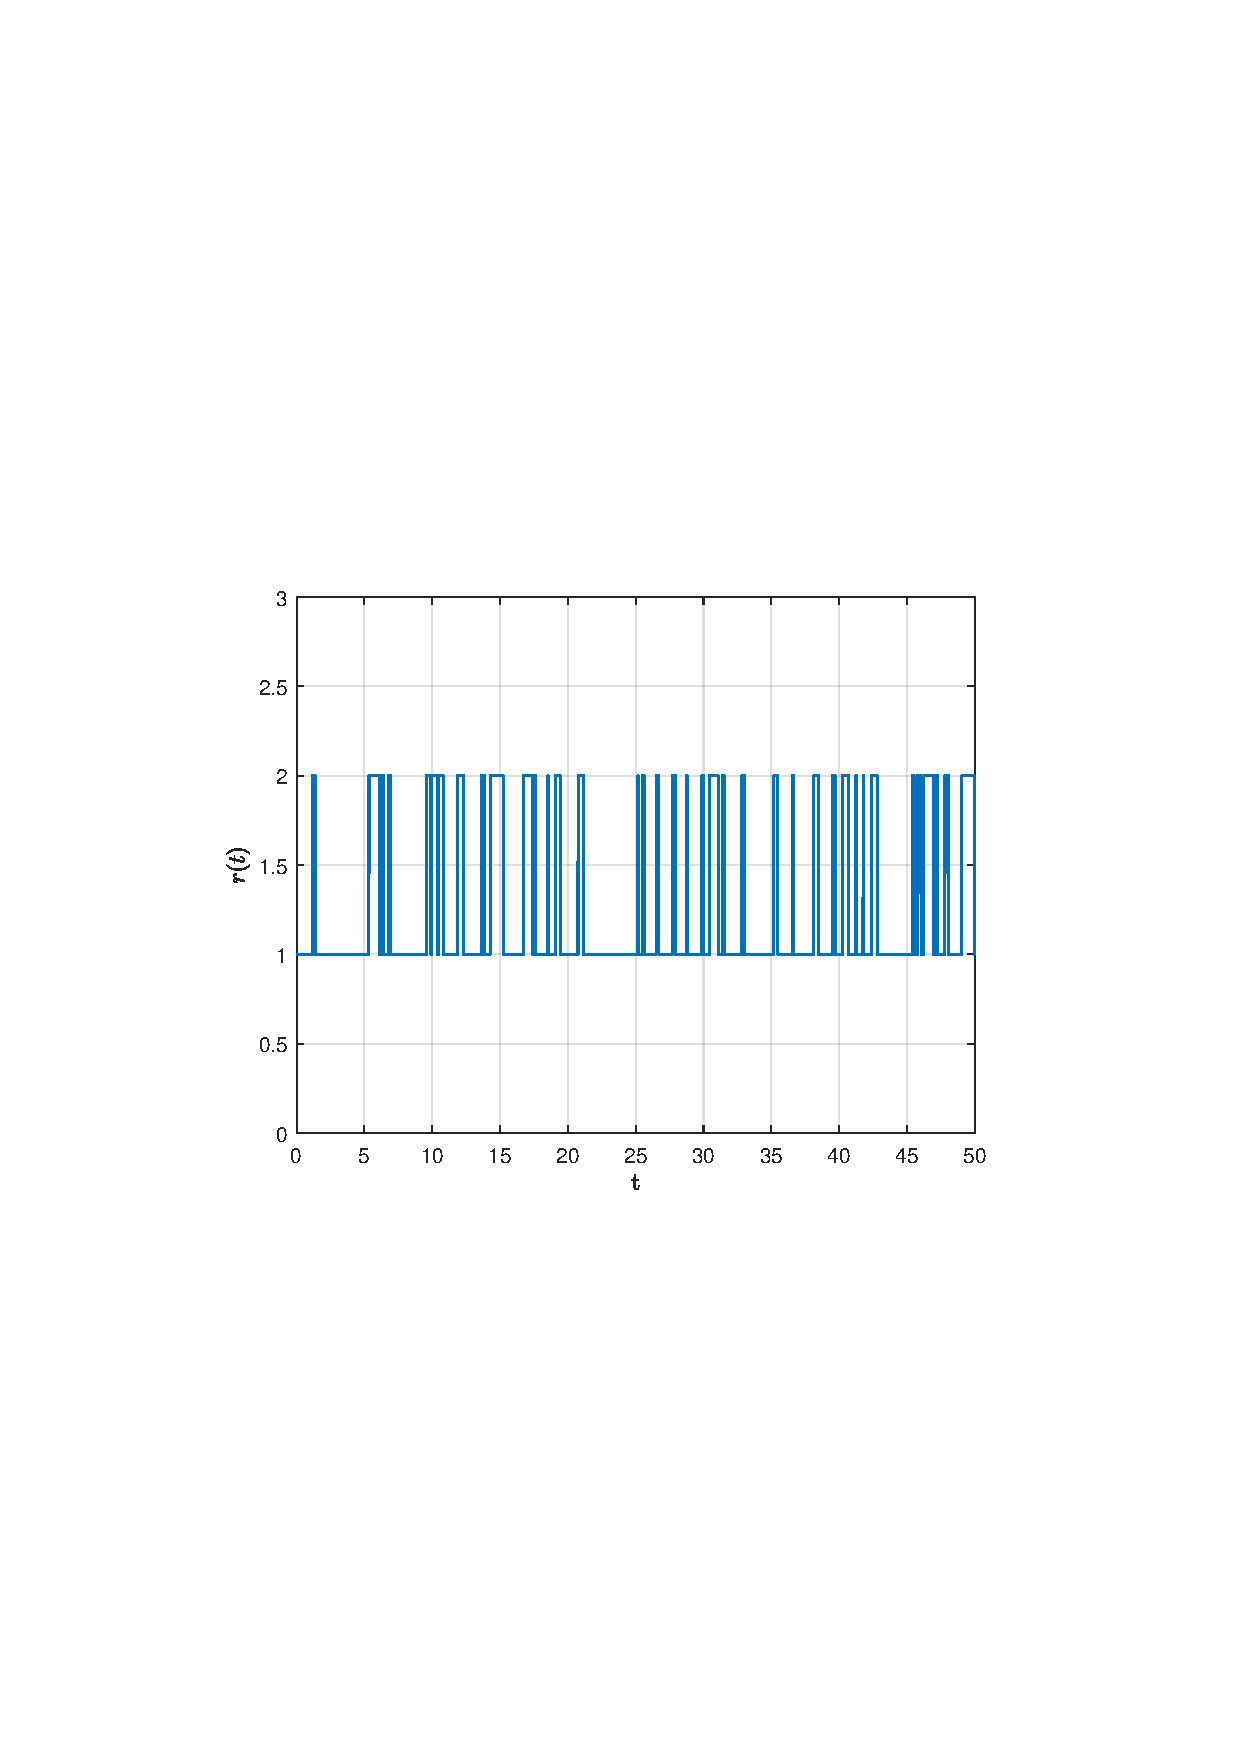
\includegraphics[width=0.9\textwidth]{figs/markov.pdf} 
		\caption{The semi-Markov switching signal.}
		\label{Fig.2}
	\end{minipage}
	\begin{minipage}{0.49\linewidth}
		\centering 
		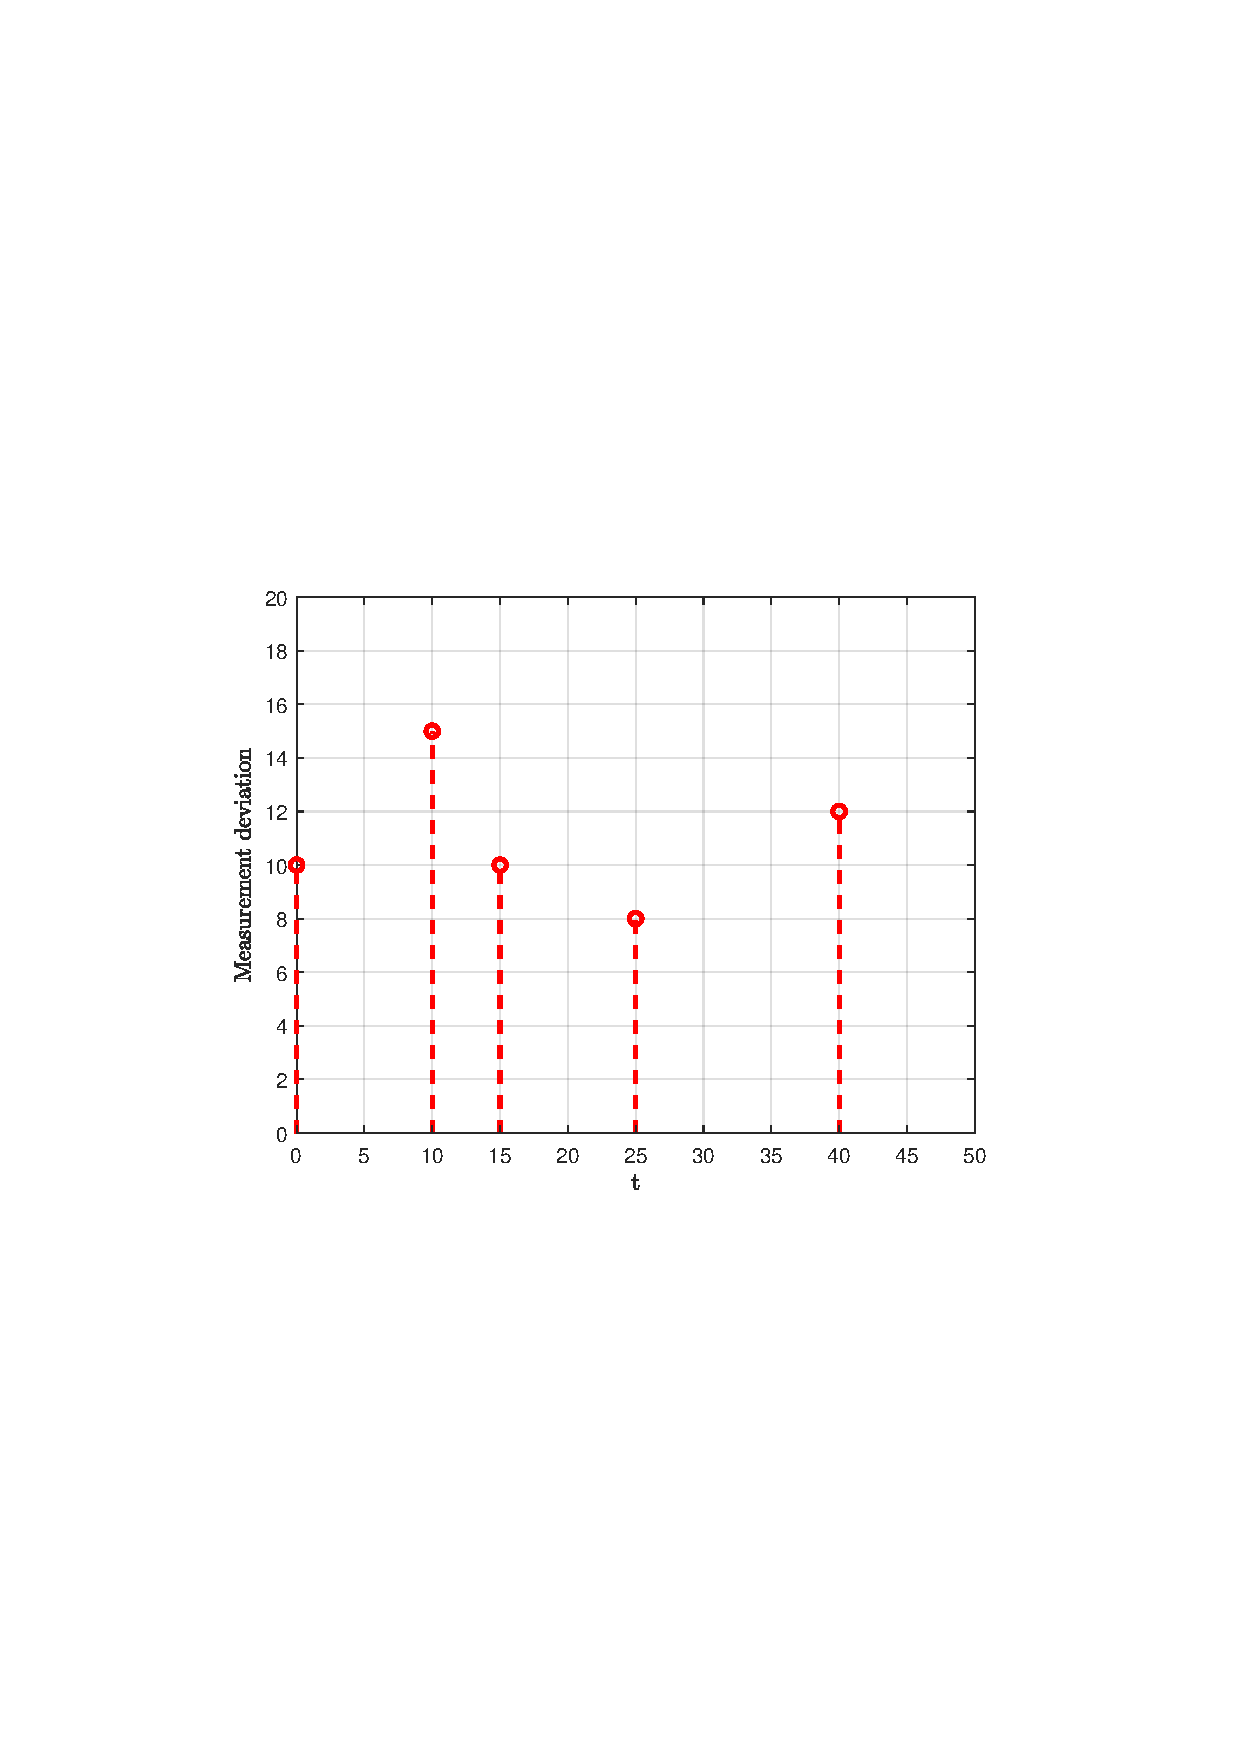
\includegraphics[width=0.9\textwidth]{figs/outlier.pdf}
		\caption{{\color{red}Measurement deviation caused by abnormal disturbance.}}
		\label{Fig.3}
	\end{minipage}
\end{figure}
\begin{figure}[H]
	\centering
	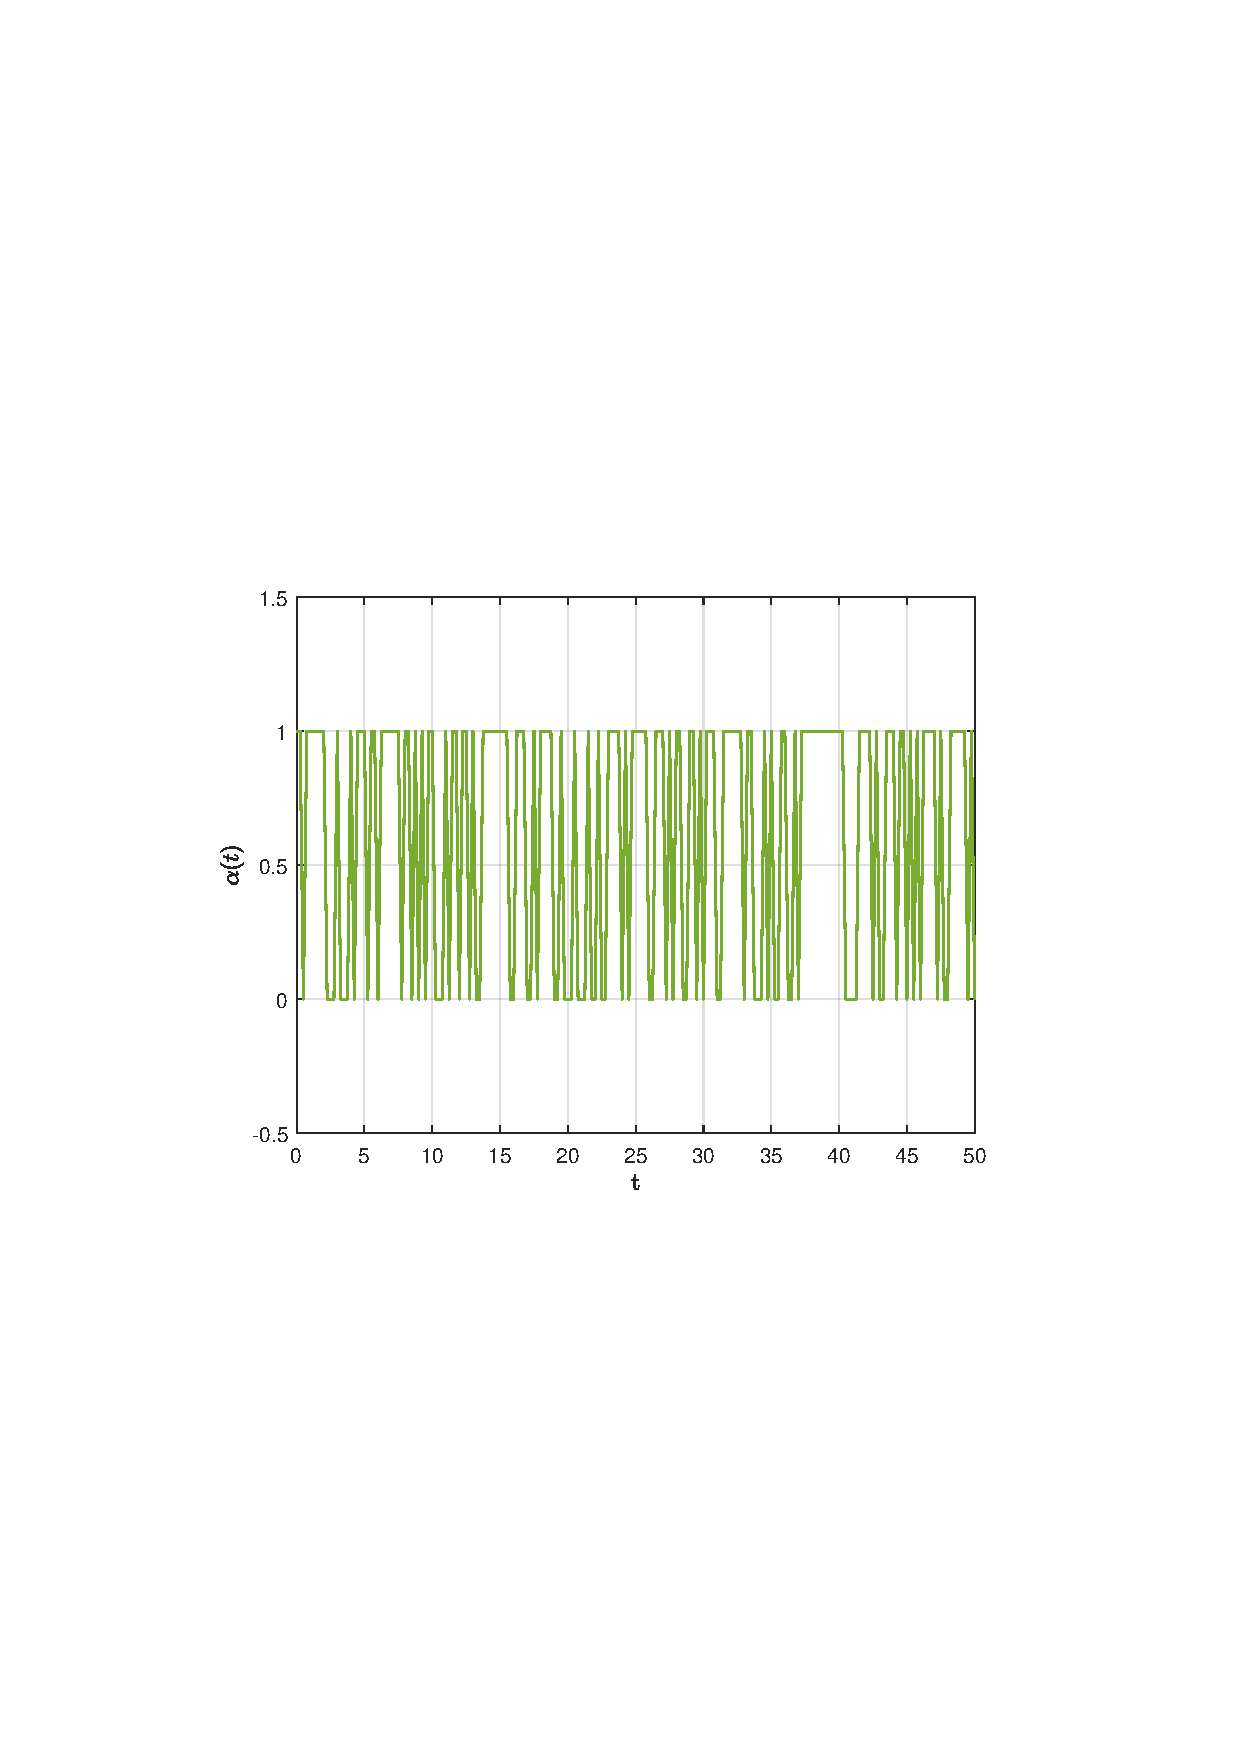
\includegraphics[width=3.5in]{figs/resilient.pdf}
	\caption{The Bernoulli stochastic variable $\alpha(t)$ with $\bar{\alpha}=0.6$.}
	\label{Fig.4}
\end{figure}
\begin{figure}[H]
	\centering
	\subfigure[]{
		\label{Fig.5.a}
		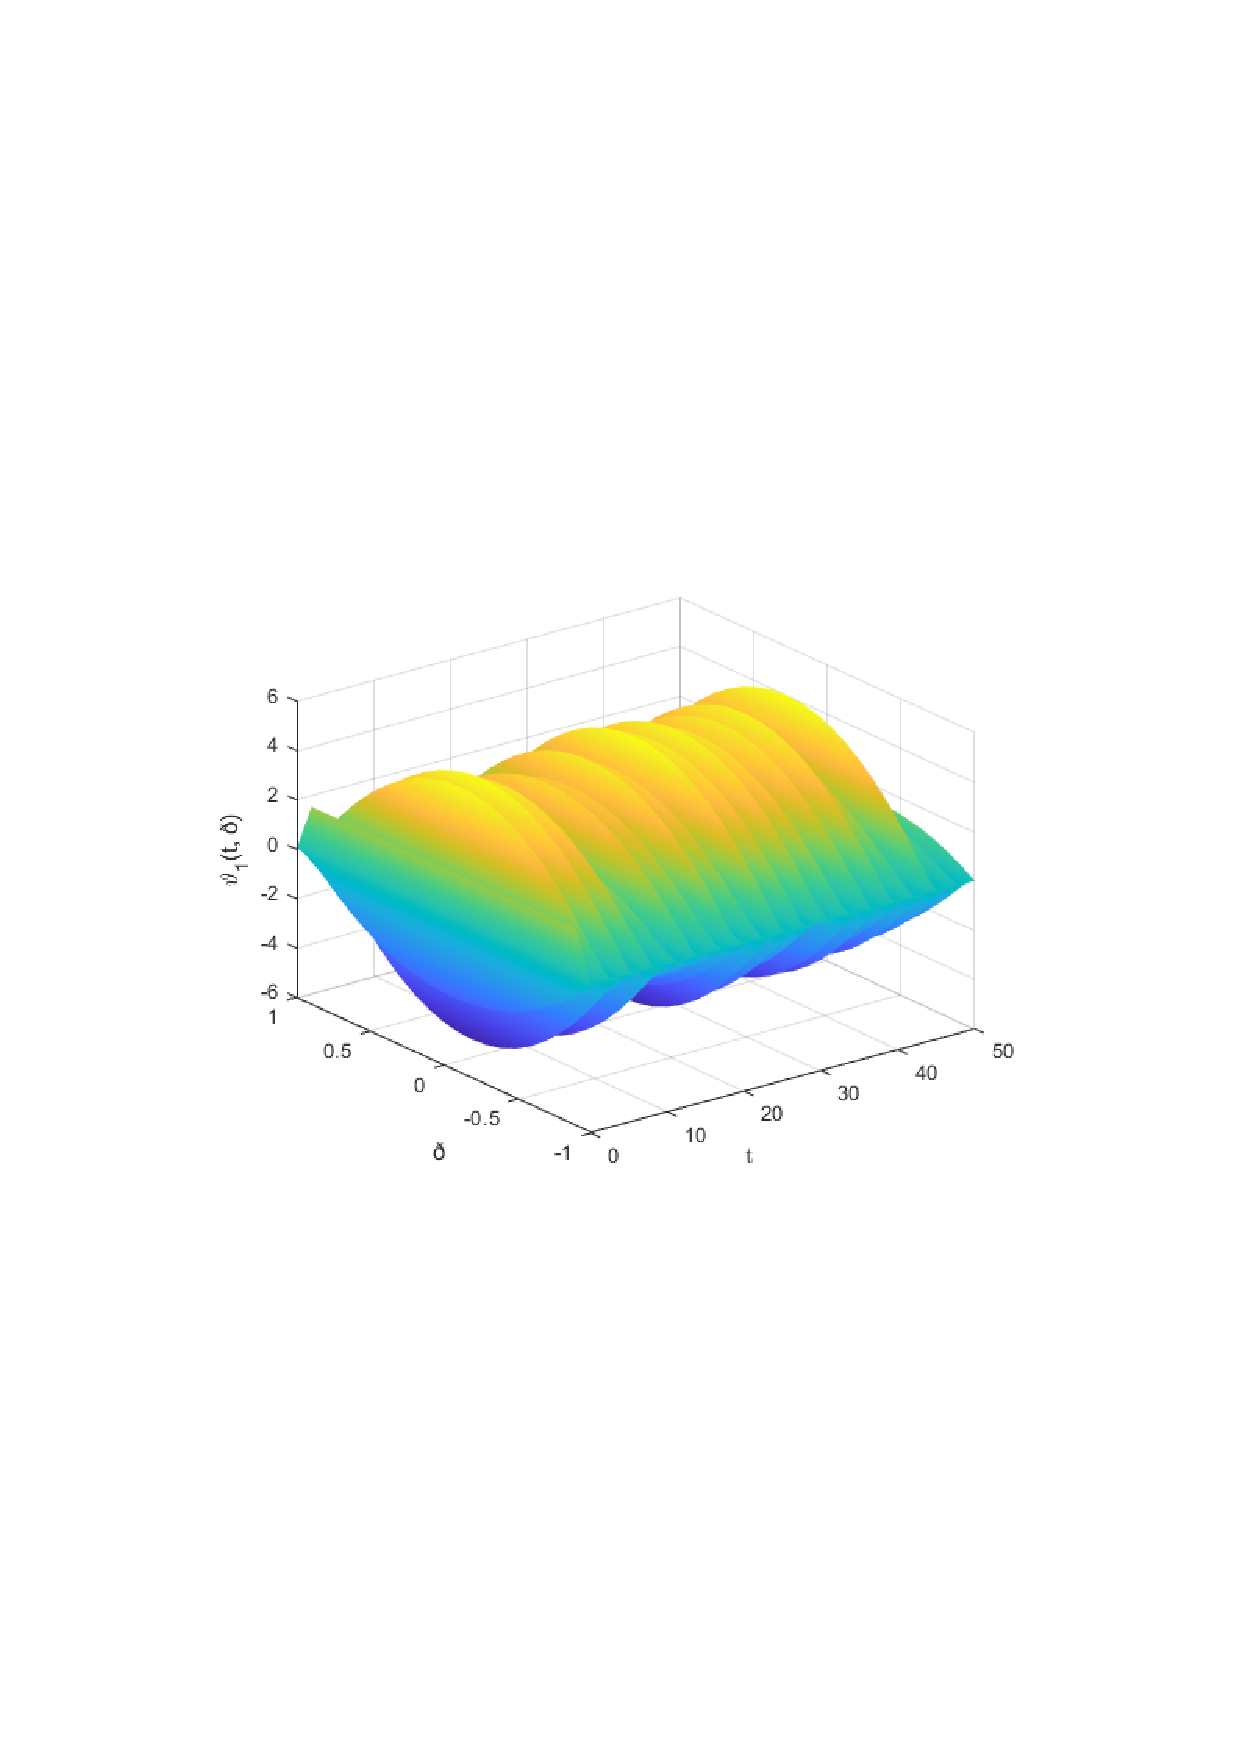
\includegraphics[width=0.45\textwidth]{figs/e1-3_ne.pdf}}
	\subfigure[]{
		\label{Fig.5.b}
		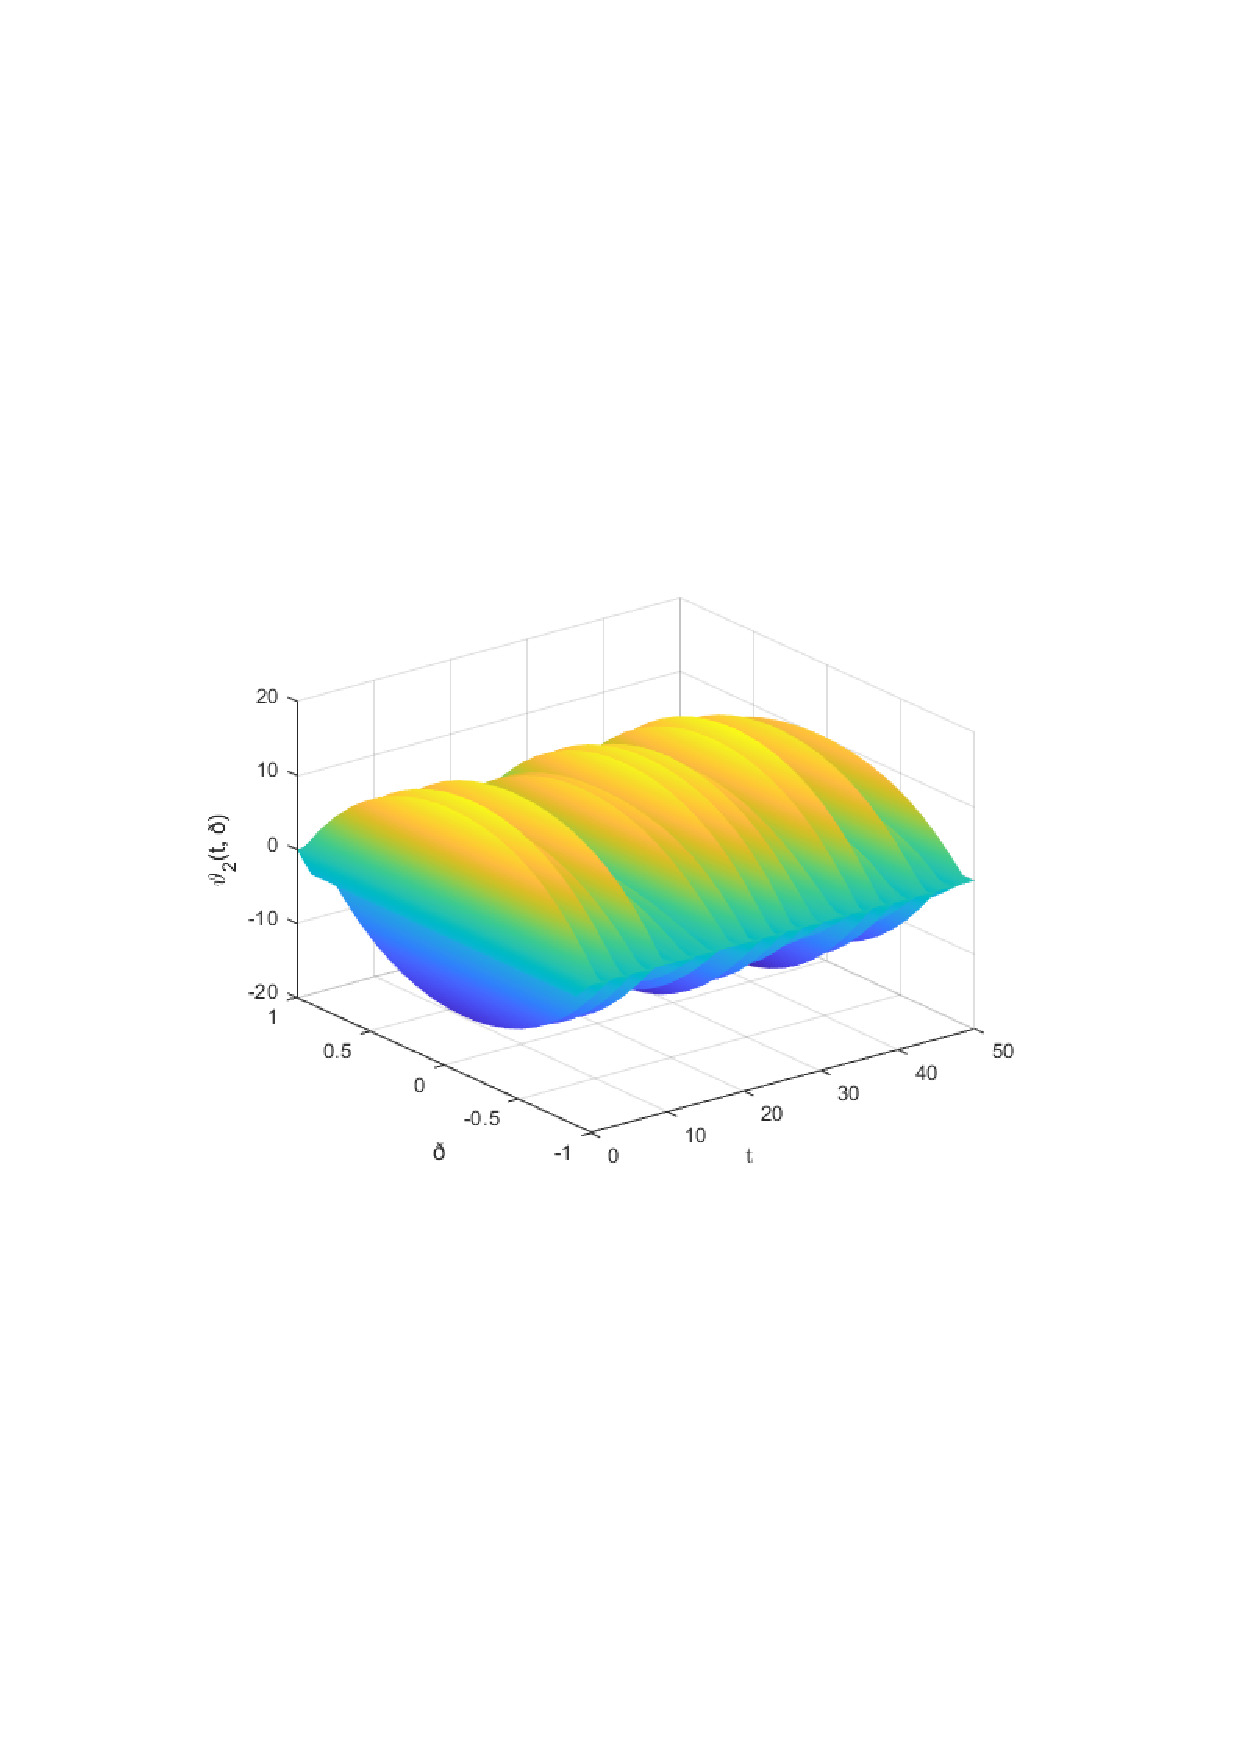
\includegraphics[width=0.45\textwidth]{figs/e2-3_ne.pdf}}
	\caption{The open-loop error trajectories in Example \ref{example1}. (a) $\vartheta_1(t,\eth)$. (b) $\vartheta_2(t,\eth)$.}
	\label{Fig.5}
\end{figure}

\begin{figure}[H]
	\centering
	\subfigure[]{
		\label{Fig.6.a}
		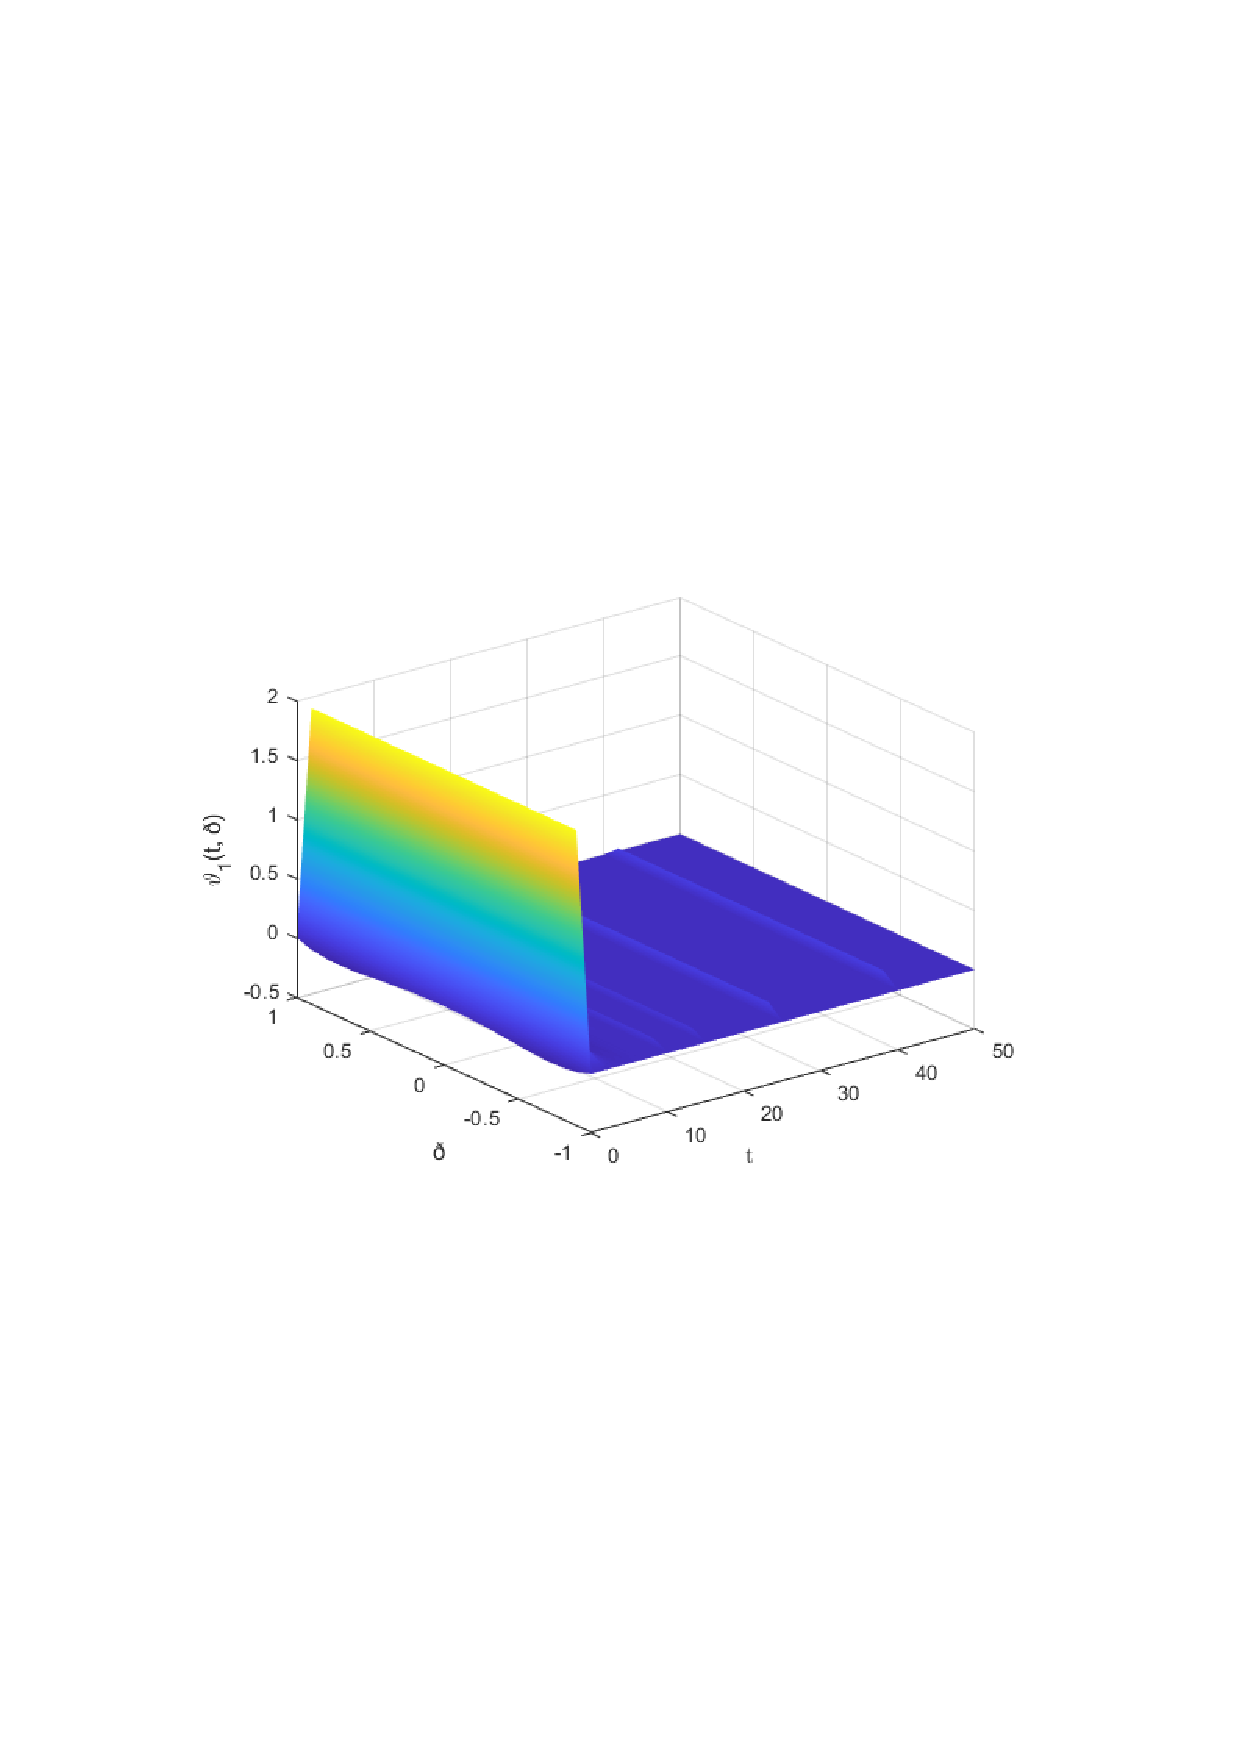
\includegraphics[width=0.45\textwidth]{figs/e1-3_e.pdf}}
	\subfigure[]{
		\label{Fig.6.b}
		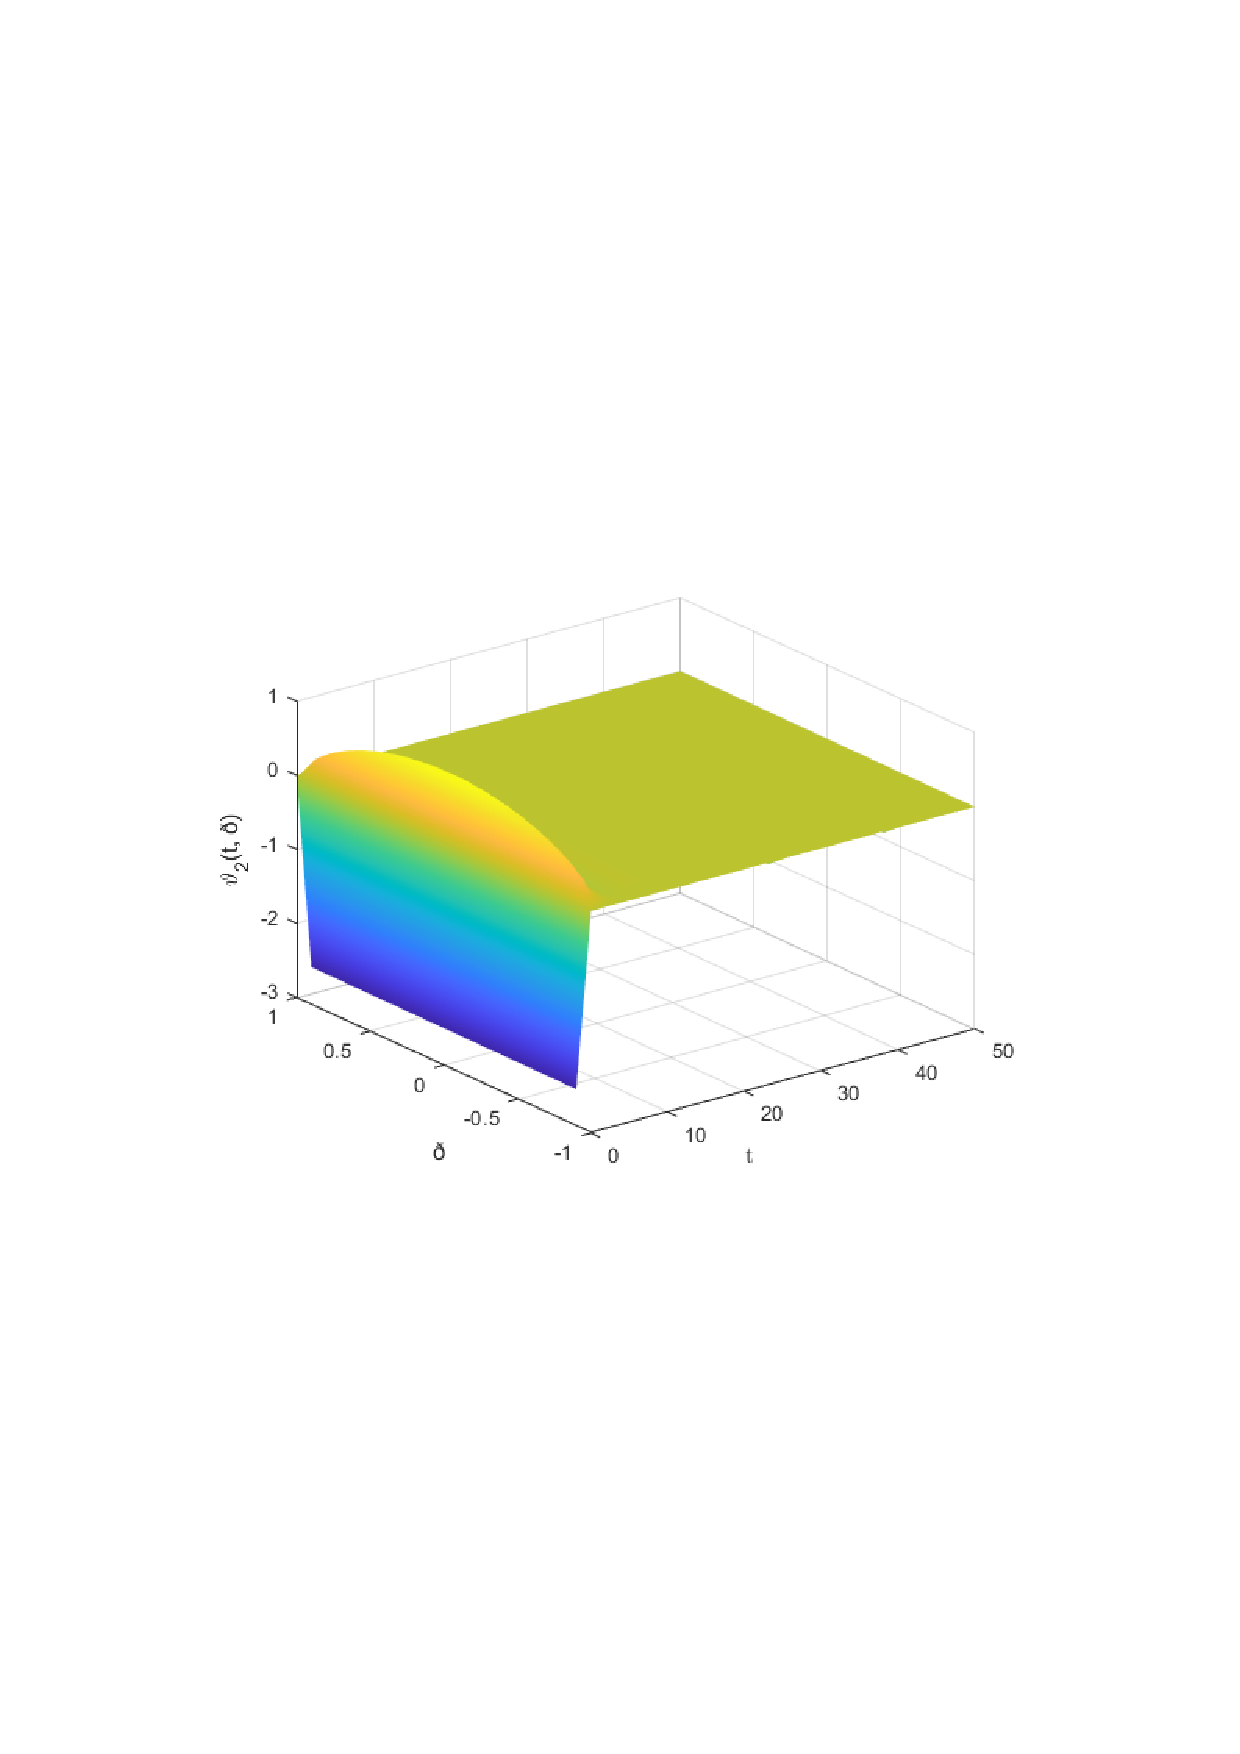
\includegraphics[width=0.45\textwidth]{figs/e2-3_e.pdf}}
	\caption{The closed-loop error trajectories in Example \ref{example1}. (a) $\vartheta_1(t,\eth)$. (b) $\vartheta_2(t,\eth)$.}
	\label{Fig.6}
\end{figure}


\begin{figure}[H]
	\centering
	\subfigure[]{
		\label{Fig.7.a}
		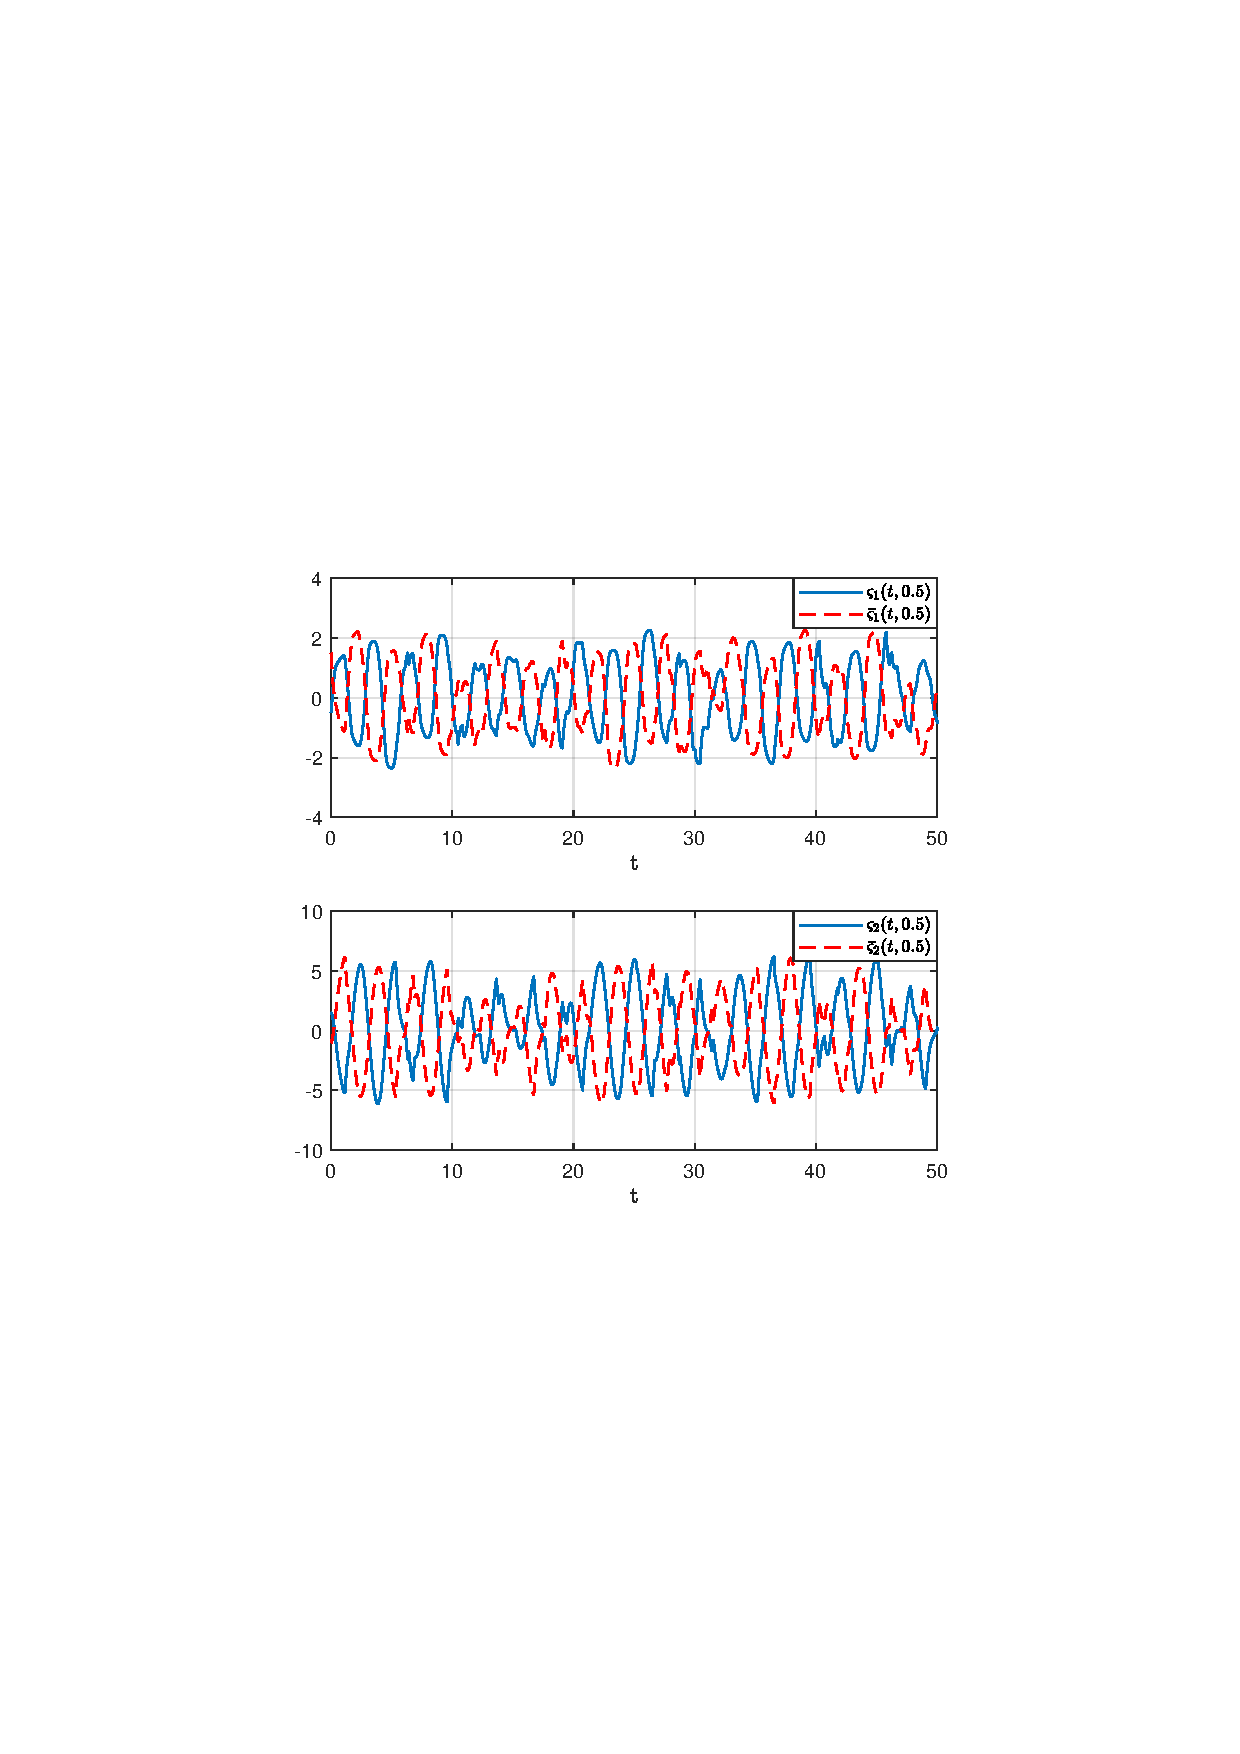
\includegraphics[width=0.45\textwidth]{figs/z1z2_ne.pdf}}
	\subfigure[]{
		\label{Fig.7.b}
		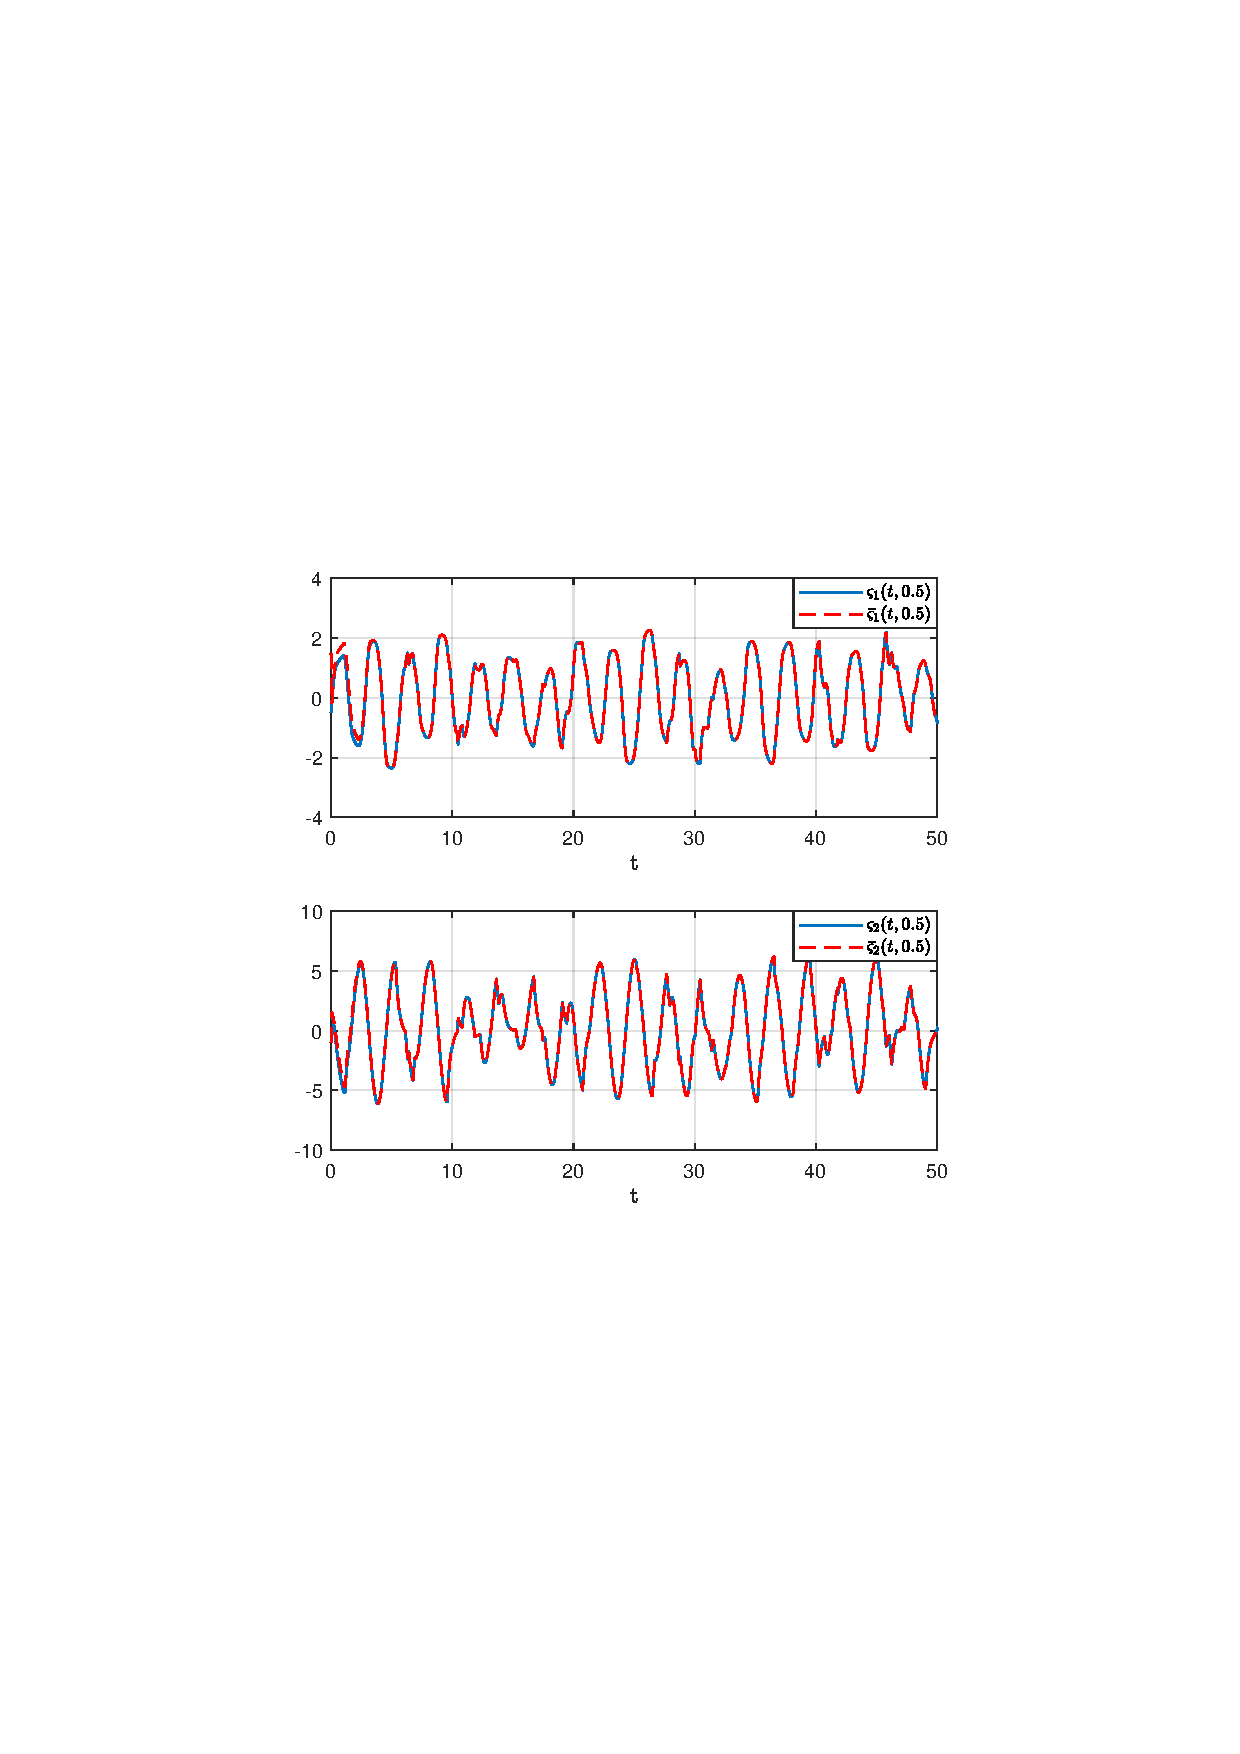
\includegraphics[width=0.45\textwidth]{figs/z1z2.pdf}}
	\caption{The real and estimated state trajectories in Example \ref{example1}. (a) open-loop. (b) closed-loop.}
	\label{Fig.7}
\end{figure}
\begin{figure}[H]
	\centering
	\subfigure[]{
		\label{Fig.8.a}
		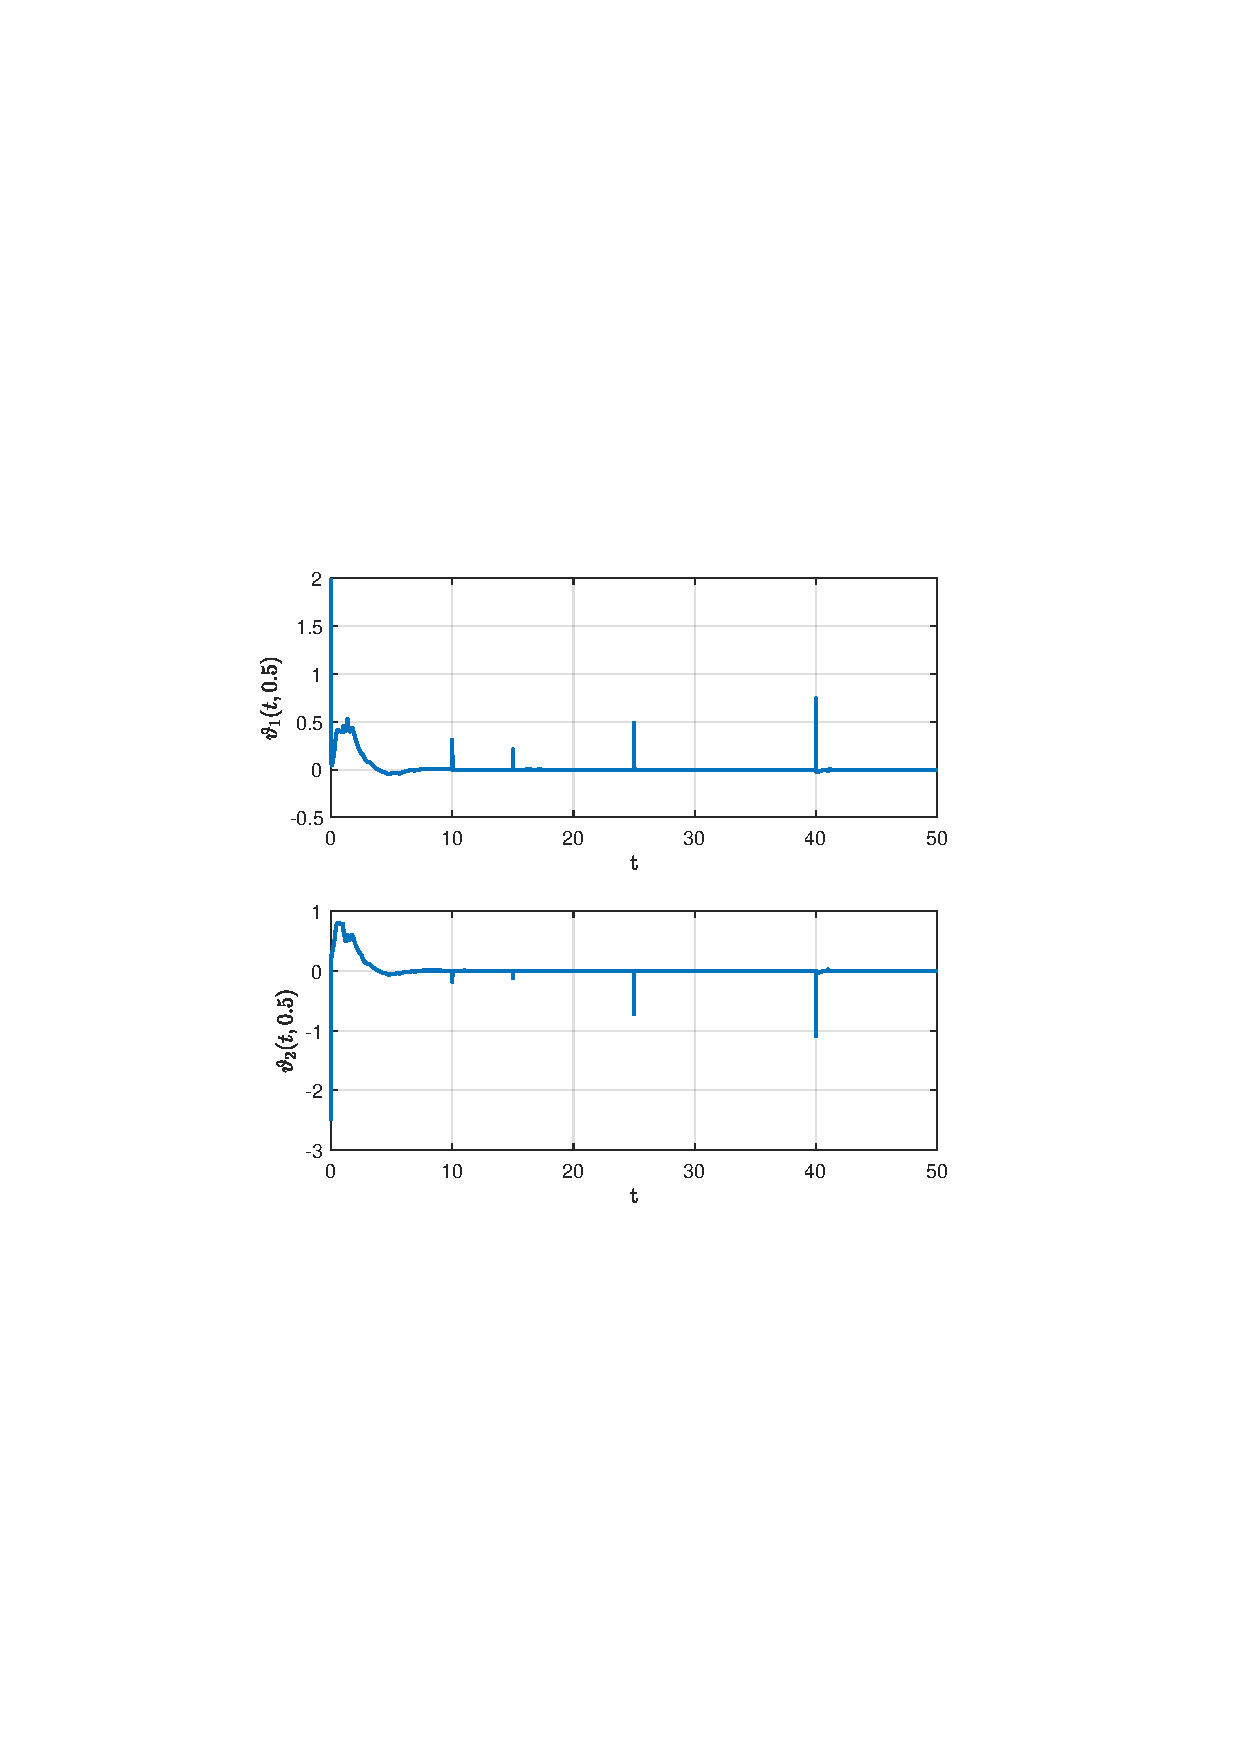
\includegraphics[width=0.45\textwidth]{figs/e1e2_nsf.pdf}}
	\subfigure[]{
		\label{Fig.8.b}
		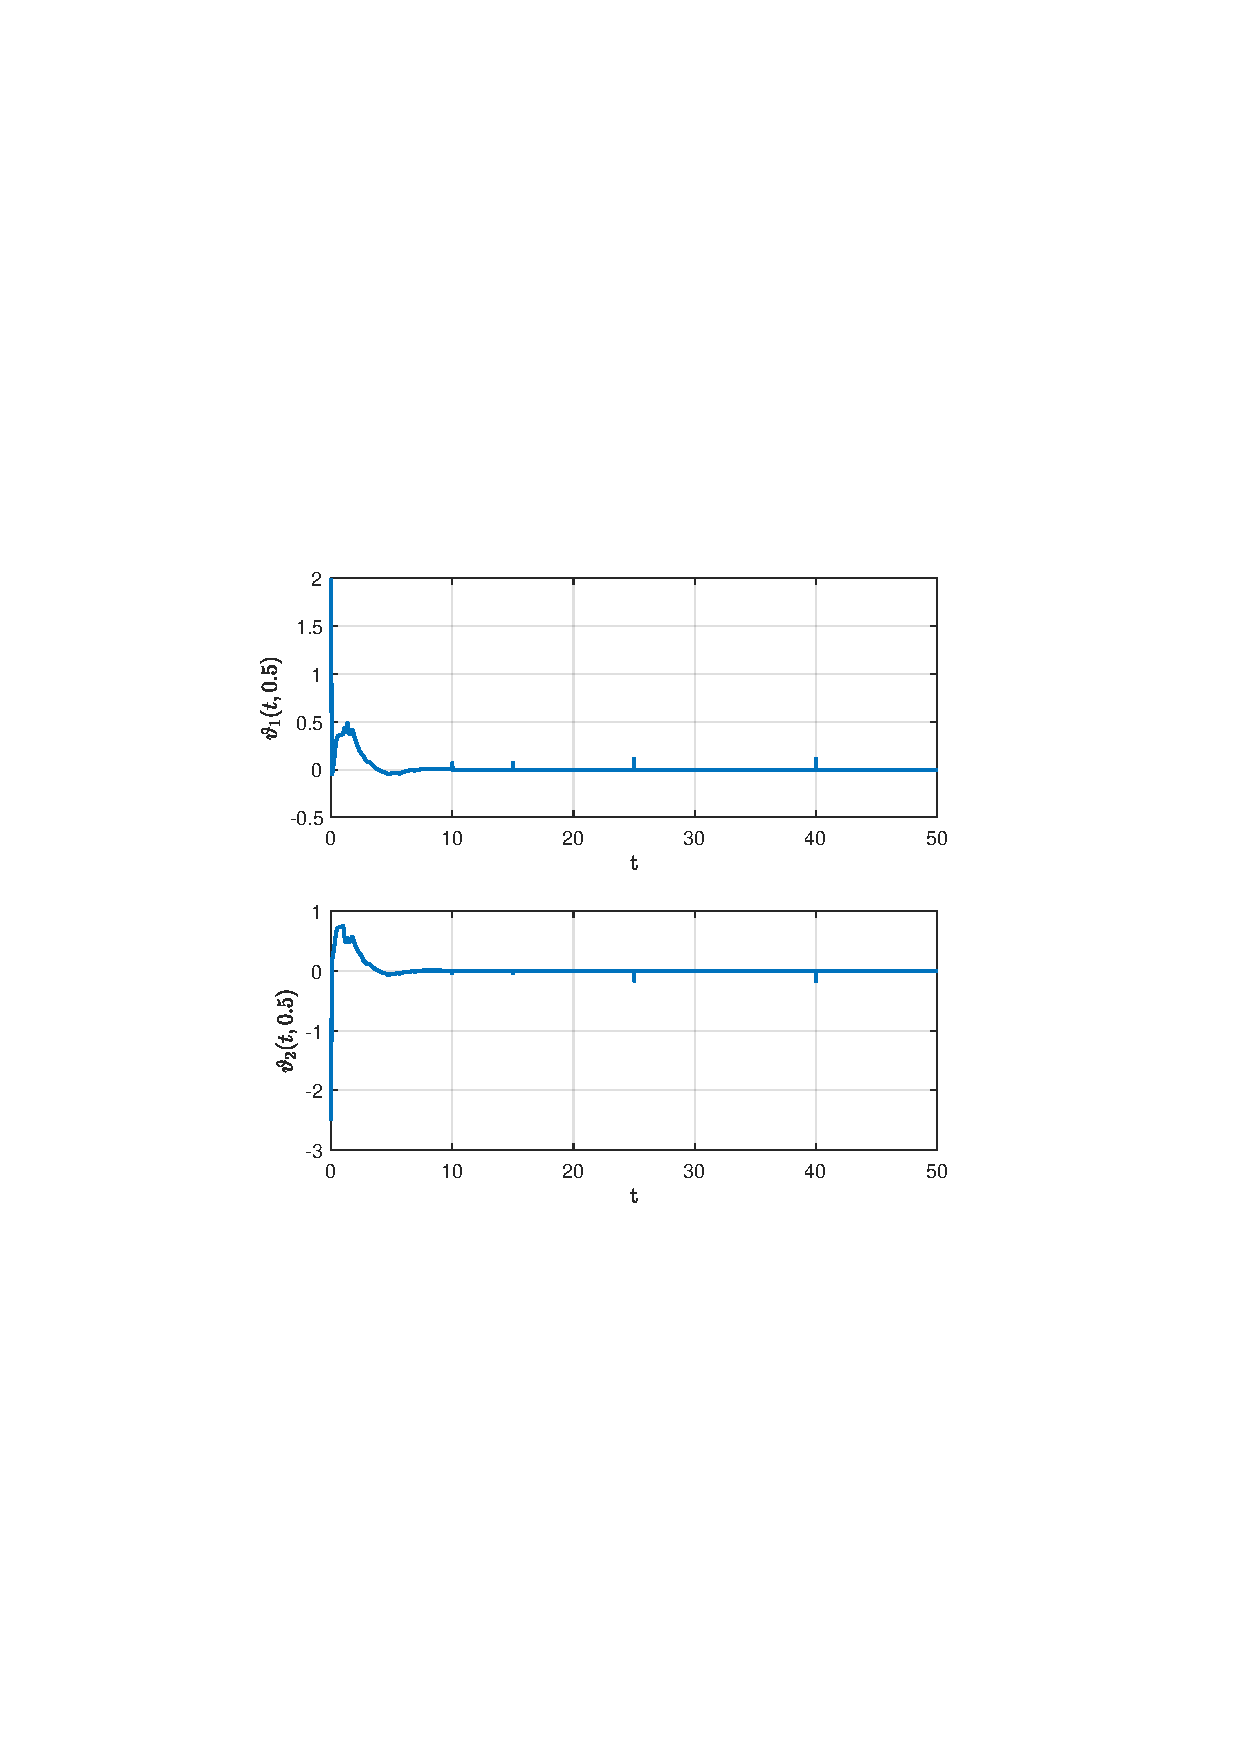
\includegraphics[width=0.45\textwidth]{figs/e1e2_sf.pdf}}
	\caption{The error trajectories at $\eth=0.5$ in Example \ref{example1}. (a) with resilient estimator. (b) with ORSE.}
	\label{Fig.8}
\end{figure}

\begin{table}[h]
	\centering
	\caption{{\color{red}The estimation error caused by measurement outliers with $\bar{\alpha}=0.6$.}}
	\label{tab1}
	\begin{tabular}{c|c|c|c|c|c}
		\toprule
		\multicolumn{2}{c|}{Time}& 10 & 15 & 25 & 40 \\ \hline
		\multicolumn{2}{c|}{Measurement outlier} &{\color{red}$y_i(10,0.5) + 15$} & {\color{red}$y_i(15,0.5)+10$} & {\color{red}$y_i(25,0.5)+8$} & {\color{red}$y_i(40,0.5)+12$} \\ \hline
		\multirow{2}*{Resilient state estimator}& $\vartheta_1(t,0.5)$ & 0.313 & 0.211 & 0.492 & 0.744 \\ \cline{2-6}
		~ & $\vartheta_2(t,0.5)$ & -0.186 & -0.125 & -0.726 & -1.094 \\ \hline
		\multirow{2}*{ORSE} & $\vartheta_1(t,0.5)$ & 0.071 & 0.070 & 0.112 & 0.113 \\ \cline{2-6}
		~ & $\vartheta_2(t,0.5)$ & -0.040 & -0.041 & -0.165 & -0.166 \\ \bottomrule
	\end{tabular}
\end{table}

When the saturation function is removed, the state estimator \eqref{equ3} degenerates to a standard resilient state estimator. The error state trajectories under this estimator are shown in Fig.~\ref{Fig.8.a}, where it is evident that measurement outliers lead to larger estimation errors, preventing accurate state estimation. In contrast, Fig.~\ref{Fig.8.b} depicts the error state trajectories under the ORSE, it is obvious that the estimated state remains reliable. When measurement outliers occur, the specific estimation errors of both the resilient estimator and the ORSE are summarized in Table.~\ref{tab1}-\ref{tab3}, further confirming that the ORSE effectively mitigates the impact of outliers on state estimation accuracy.
\begin{table}[h]
	\centering
	{\color{red}
	\caption{{\color{red}The estimation error caused by measurement outliers with $\bar{\alpha}=0.5$.}}
	\label{tab2}
	\begin{tabular}{c|c|c|c|c|c}
		\toprule
		\multicolumn{2}{c|}{Time}& 10 & 15 & 25 & 40 \\ \hline
		\multicolumn{2}{c|}{Measurement outlier} &$y_i(10,0.5) + 15$ & $y_i(15,0.5)+10$ & $y_i(25,0.5)+8$ & $y_i(40,0.5)+12$ \\ \hline
		\multirow{2}*{Resilient state estimator}& $\vartheta_1(t,0.5)$ & 0.915 & 0.619 & 0.491 & 0.743 \\ \cline{2-6}
		~ & $\vartheta_2(t,0.5)$ & -0.186 & -0.135& -0.910 & -1.093 \\ \hline
		\multirow{2}*{ORSE} & $\vartheta_1(t,0.5)$ & 0.111 &0.113 & 0.112 & 0.113\\ \cline{2-6}
		~ & $\vartheta_2(t,0.5)$ & -0.165 &-0.166 & -0.165 & -0.166 \\ \bottomrule
	\end{tabular}
}
\end{table}

\begin{table}[h]
	\centering
	{\color{red}
	\caption{{\color{red}The estimation error caused by measurement outliers with $\bar{\alpha}=0.8$.}}
	\label{tab3}
	\begin{tabular}{c|c|c|c|c|c}
		\toprule
		\multicolumn{2}{c|}{Time}&10 & 15 & 25 & 40 \\ \hline
		\multicolumn{2}{c|}{Measurement outlier} &$y_i(10,0.5) + 15$ & $y_i(15,0.5)+10$ & $y_i(25,0.5)+8$ & $y_i(40,0.5)+12$ \\ \hline
		\multirow{2}*{Resilient state estimator}& $\vartheta_1(t,0.5)$& 0.919 & 0.214 & 0.168 & 0.746 \\ \cline{2-6}
		~ & $\vartheta_2(t,0.5)$ & -1.357& -0.126 & -0.100 & -1.095 \\ \hline
		\multirow{2}*{ORSE} & $\vartheta_1(t,0.5)$ & 0.112 & 0.072 & 0.070 & 0.113 \\ \cline{2-6}
		~ & $\vartheta_2(t,0.5)$ & -0.164 & -0.041 & -0.042 & -0.166 \\ \bottomrule
	\end{tabular}
}
\end{table}

\end{example}

To further demonstrate the availability, the general 3-D RDNNs with three modes is carried out in the following example.

\begin{example}	\label{example2}
	Consider three-mode semi-Markov switching RDNNs, and its parameters are given as follows:
	\begin{figure}[H]
		\centering
		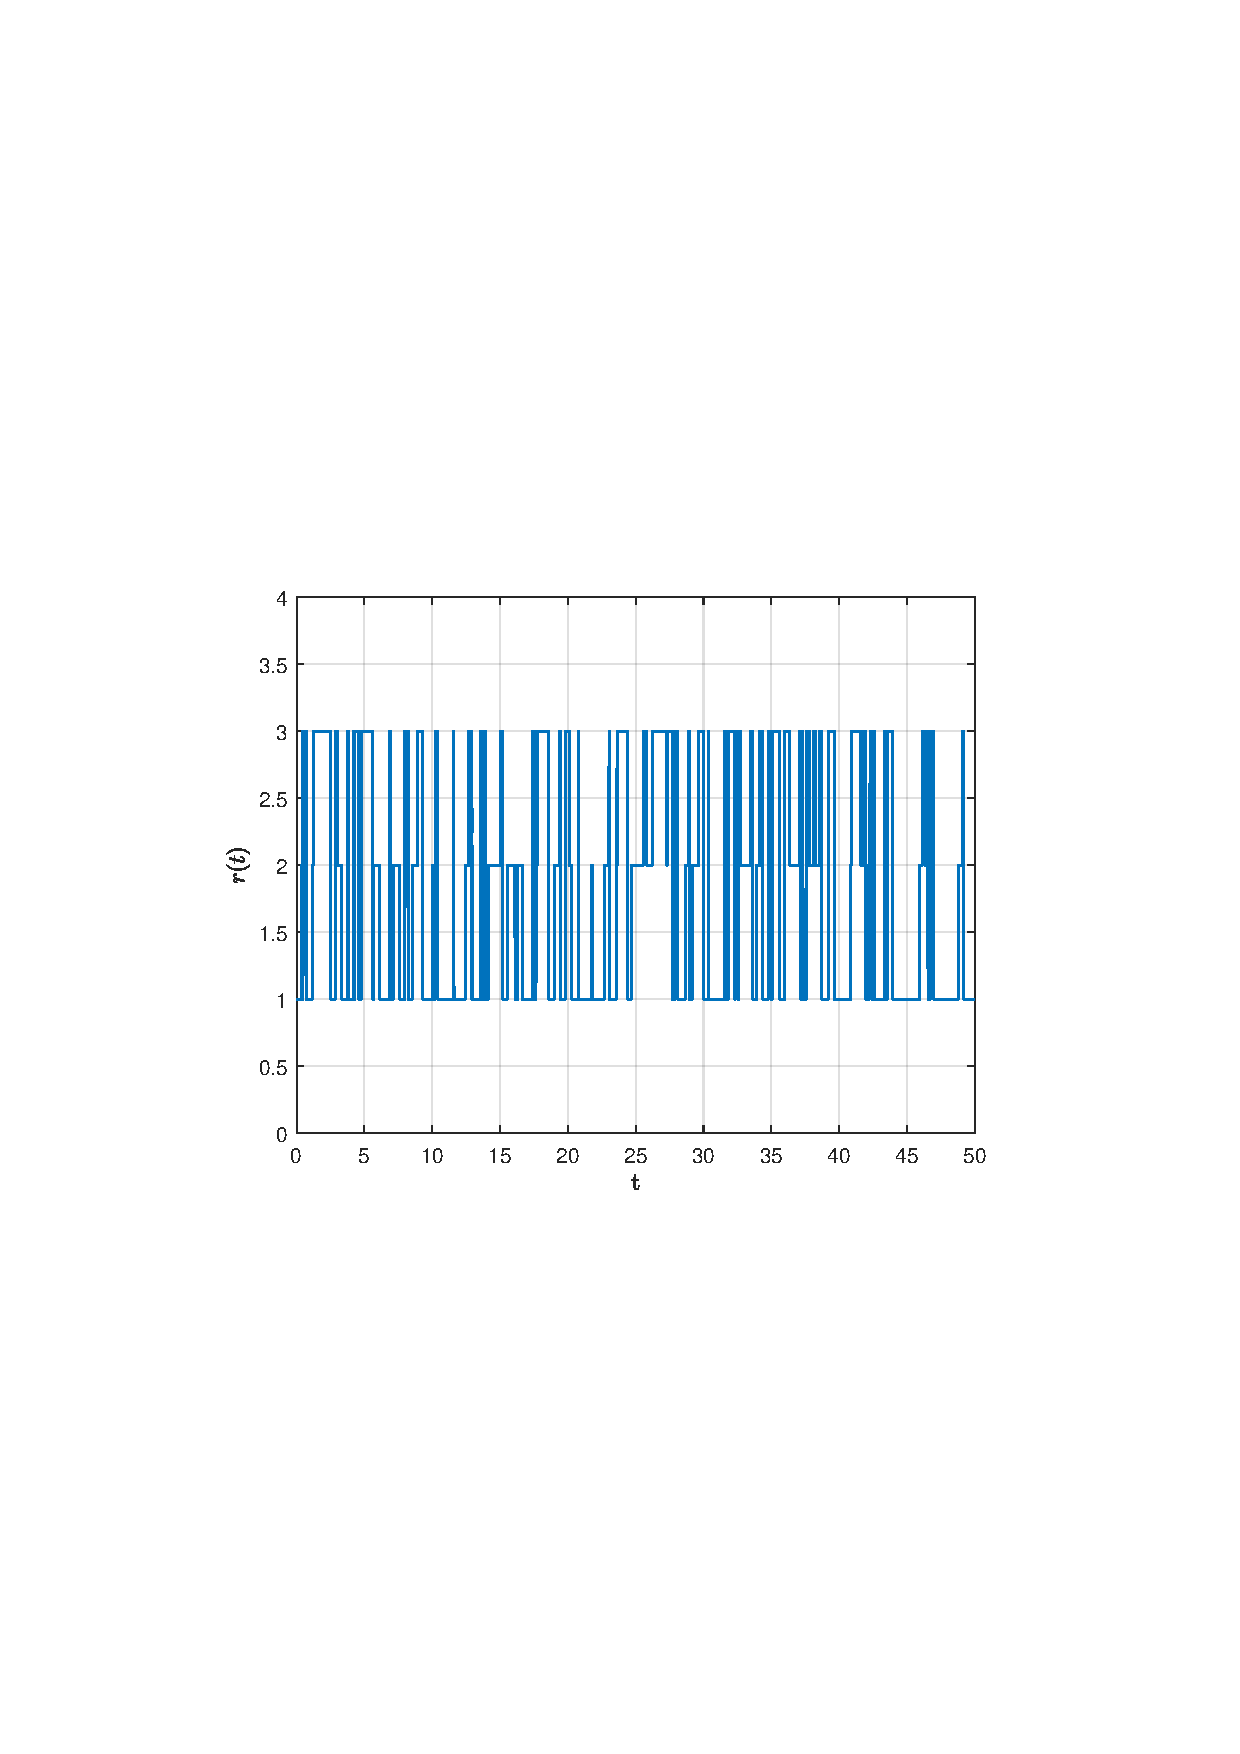
\includegraphics[width=3.5in]{figs/markov-3.pdf}
		\caption{Semi-Markov switching signal with three modes.}
		\label{Fig.9}
	\end{figure}
	\begin{align*}
		A_1=\text{diag}\left\{1,1,2\right\},
		A_2=\text{diag}\left\{1.5,1.5,1\right\},
		A_3=\text{diag}\left\{1,2,1\right\},
		D_1=\text{diag}\left\{0.3,0.3,0.3\right\},
	\end{align*}
	\begin{align*}	
		G_1=\text{diag}\left\{-1,-1\right\},
		G_2=\text{diag}\left\{-1.5,-1.5\right\},
		\mathcal{D}_1=\text{diag}\left\{0.6,0.6,0.6\right\},
		\mathcal{D}_2=\text{diag}\left\{0.3,0.3,0.3\right\},
	\end{align*}
	\begin{align*}	
		\mathcal{D}_3=\text{diag}\left\{0.5,0.5,0.5\right\},
		\mathcal{M}_1=\text{diag}\left\{0.7,0.7,0.7\right\},
		\mathcal{M}_2=\text{diag}\left\{0.9,0.9,0.9\right\},
		\mathcal{M}_3=\text{diag}\left\{0.8,0.8,0.8\right\},
	\end{align*}
	\begin{align*}
		W_{11}=\begin{bmatrix}
			2&-1&0\\1.7&1.71&1.1\\-2.5&-2.9&0.56
		\end{bmatrix},
		W_{12}=\begin{bmatrix}
			2.5&-2&0\\1.5&1.4&0.9\\-2&-2.4&0.8
		\end{bmatrix},
		W_{13}=\begin{bmatrix}
			2.1&-1.3&0\\1.6&1.1&1.8\\-1.9&-3.1&0.9
		\end{bmatrix},
		W_{21}=\begin{bmatrix}
			1&-2&0\\2&2&1\\-2.5&-3&0.7
		\end{bmatrix},
	\end{align*}	
	\begin{align*}
		W_{22}=\begin{bmatrix}
			2&-1.5&0.5\\0.7&1&2\\-1.7&-2.5&0.6
		\end{bmatrix},
		W_{23}=\begin{bmatrix}
			1.5&-0.8&0\\1.5&1.2&2.2\\-2.1&-2.8&0.4
		\end{bmatrix},
		B_1=\begin{bmatrix}
			-0.4&-0.2&0\\0&-0.4&0\\0&0&-0.4
		\end{bmatrix},
		B_2=\text{diag}\left\{-0.5,-0.5,-0.5\right\},
	\end{align*}
	\begin{align*}
		B_3=\text{diag}\left\{-0.6,-0.6,-0.6\right\},
		\mathcal{J}_1=\text{diag}\left\{0.5,0.5,0.5\right\},
		\mathcal{J}=\text{diag}\left\{1.5,1.5,1.5\right\},
		J_1(t)=\begin{bmatrix}
			\sin(t)\\\cos(t)\\-\sin(t)
		\end{bmatrix},
		J_2(t)=\begin{bmatrix}
			\cos(t)\\\sin(t)\\-\cos(t)
		\end{bmatrix},	
	\end{align*}
	\begin{align*}
		J_3(t)=\begin{bmatrix}
			-\cos(t)\\-\sin(t)\\\cos(t)
		\end{bmatrix},	
		\omega(t,\eth)=\begin{bmatrix}
			5\mathrm{e}^{-0.5t}\sin(t)\\5\mathrm{e}^{-0.5t}\sin(t)\\5\mathrm{e}^{-0.5t}\sin(t)
		\end{bmatrix}.
	\end{align*}
	
In addition, define $f_i(e_i)=\frac{1}{2}\left(\lvert e_i+1 \rvert - \lvert e_i-1 \rvert\right)$ $(i=1,2,3)$, from Assumption 2.1, we can get $\varkappa_i^-=0$ and $\varkappa_i^+=1$. Furthermore, similar to Example \ref{example1}, let $\hbar \sim$ weibull$(1,2)$ for $u=1$, $\hbar \sim$ weibull$(1,3)$ for $u=2$ and $\hbar \sim$ weibull$(1,4)$ for $u=3$, the following TR matrix and probability density function are given:
\begin{align*}
	\Gamma(\hbar)=\begin{bmatrix}
		-2\hbar&\hbar&\hbar\\0.6\hbar^2&-3\hbar^2&2.4\hbar^2\\3.2\hbar^3&0.8\hbar^3&-4\hbar^3
	\end{bmatrix},
	\mathcal{F}_u(\hbar)=\begin{cases}
		2he^{-\hbar^2}, & u=1 \\
		3h^2e^{-\hbar^3}, & u=2\\
		4h^3e^{-\hbar^4}, & u=3
	\end{cases}.
\end{align*}

\begin{figure}[H]
	\centering
	\subfigure[]{
		\label{Fig.10.a}
		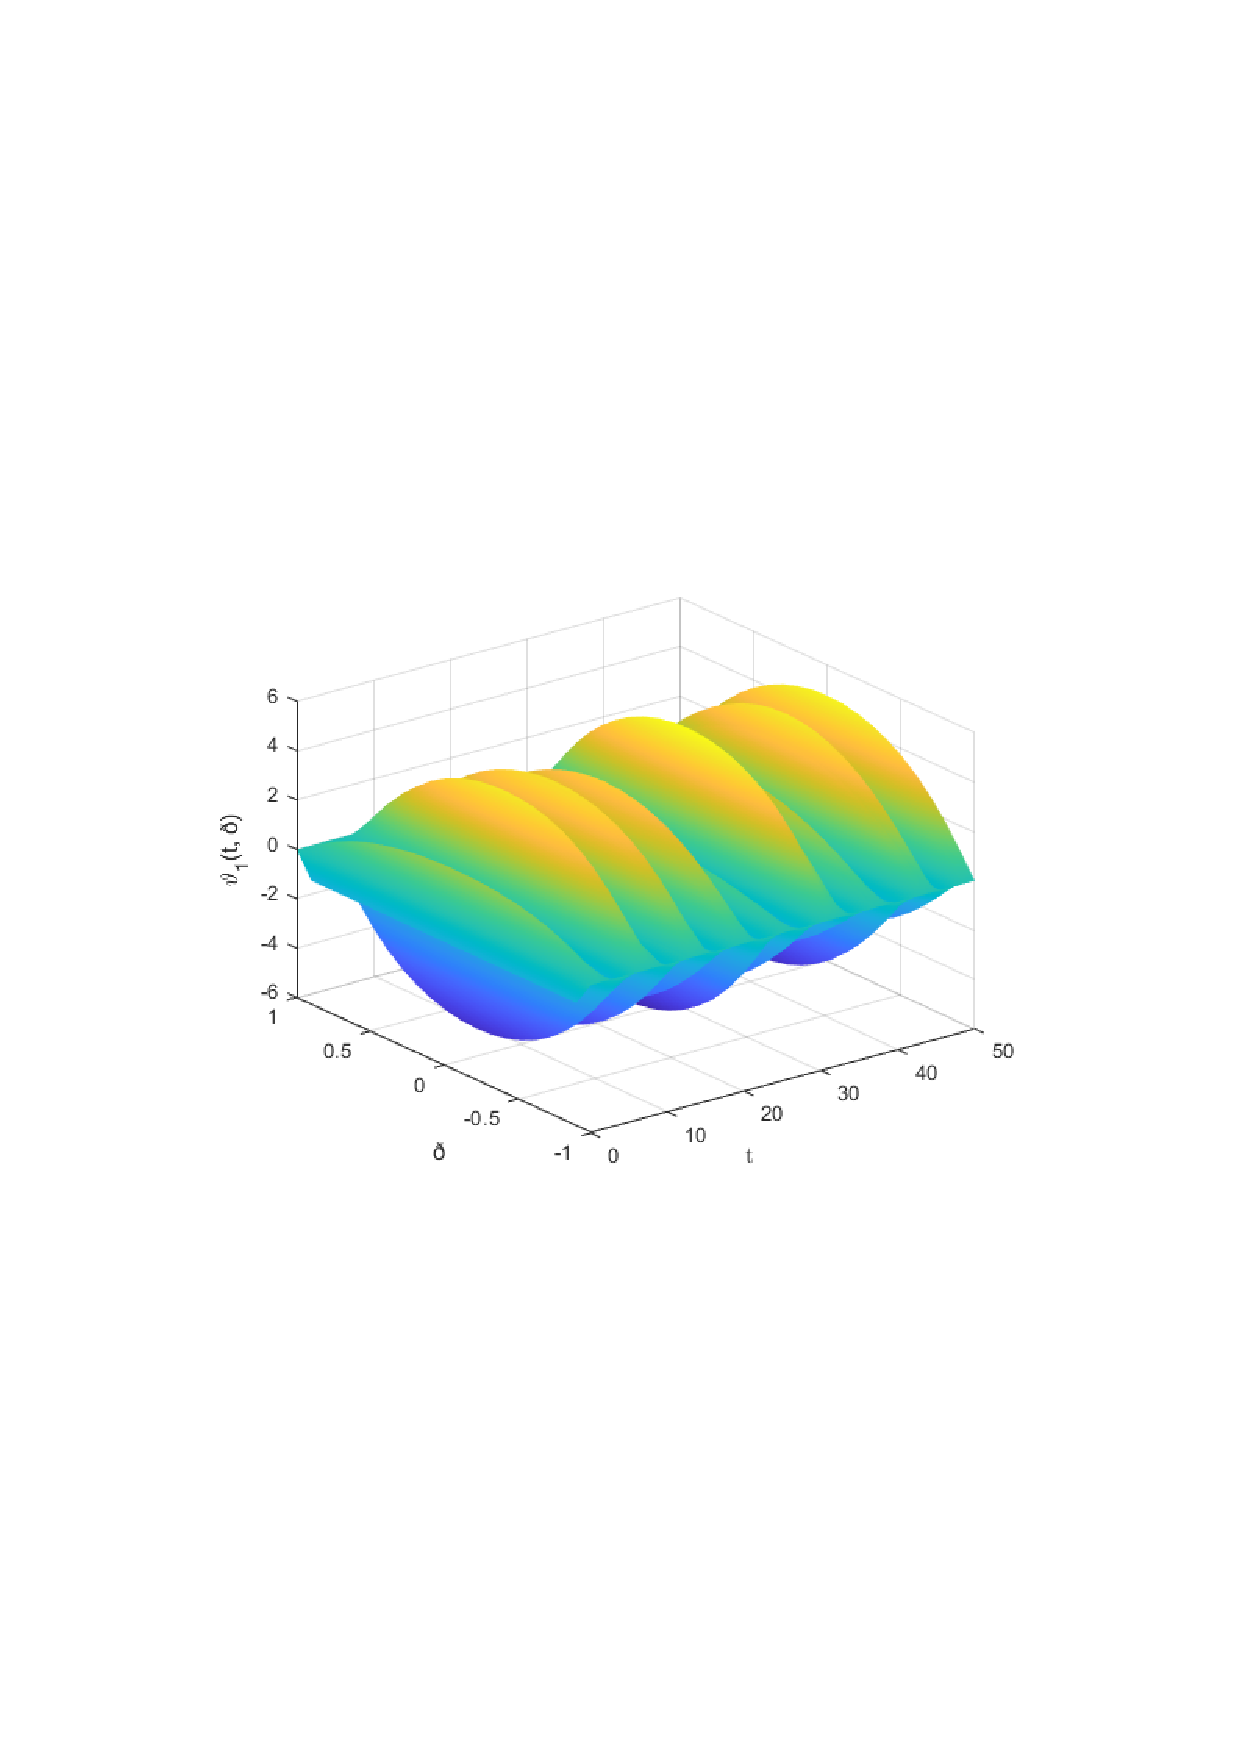
\includegraphics[width=0.45\textwidth]{figs/e1.3.pdf}}
	\vskip\baselineskip
	\subfigure[]{
		\label{Fig.10.b}
		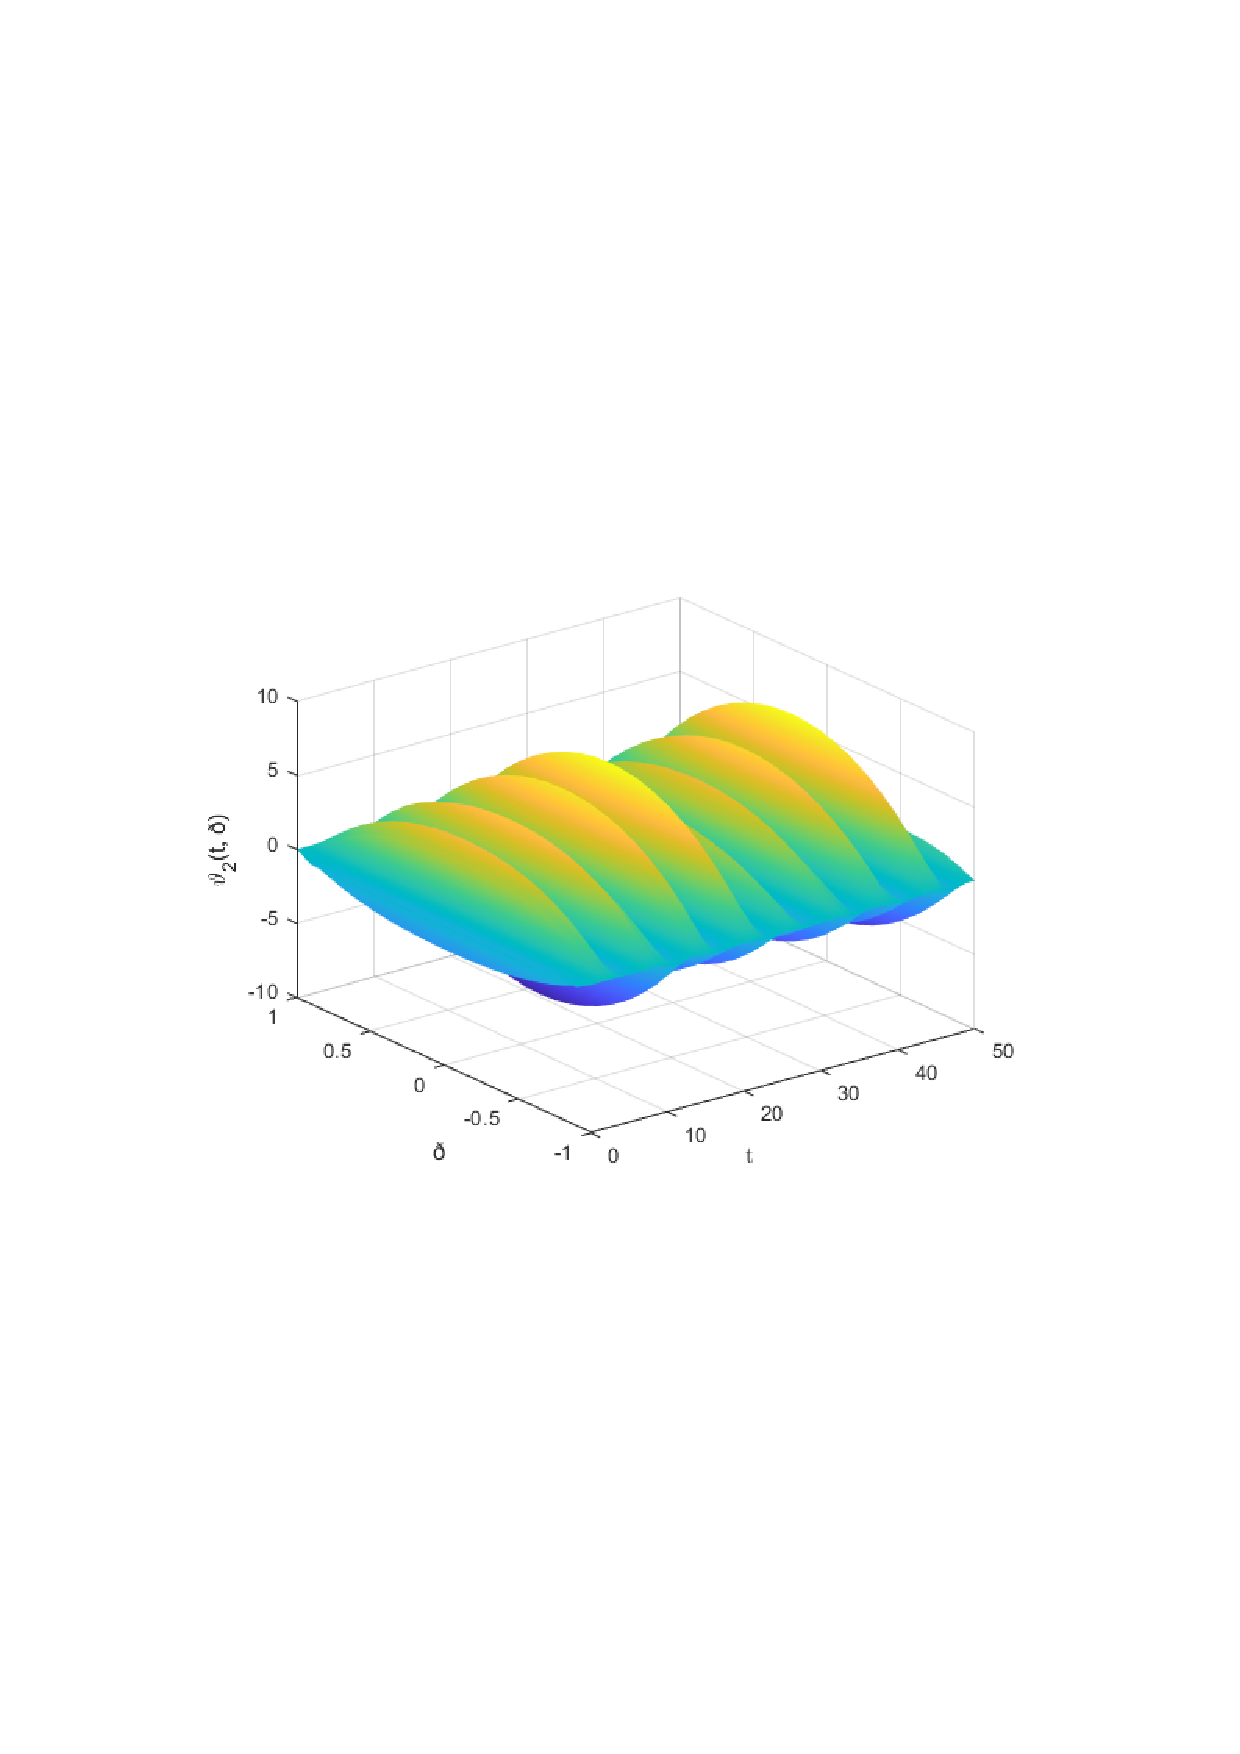
\includegraphics[width=0.45\textwidth]{figs/e2.3.pdf}}
	\subfigure[]{
		\label{Fig.10.c}
		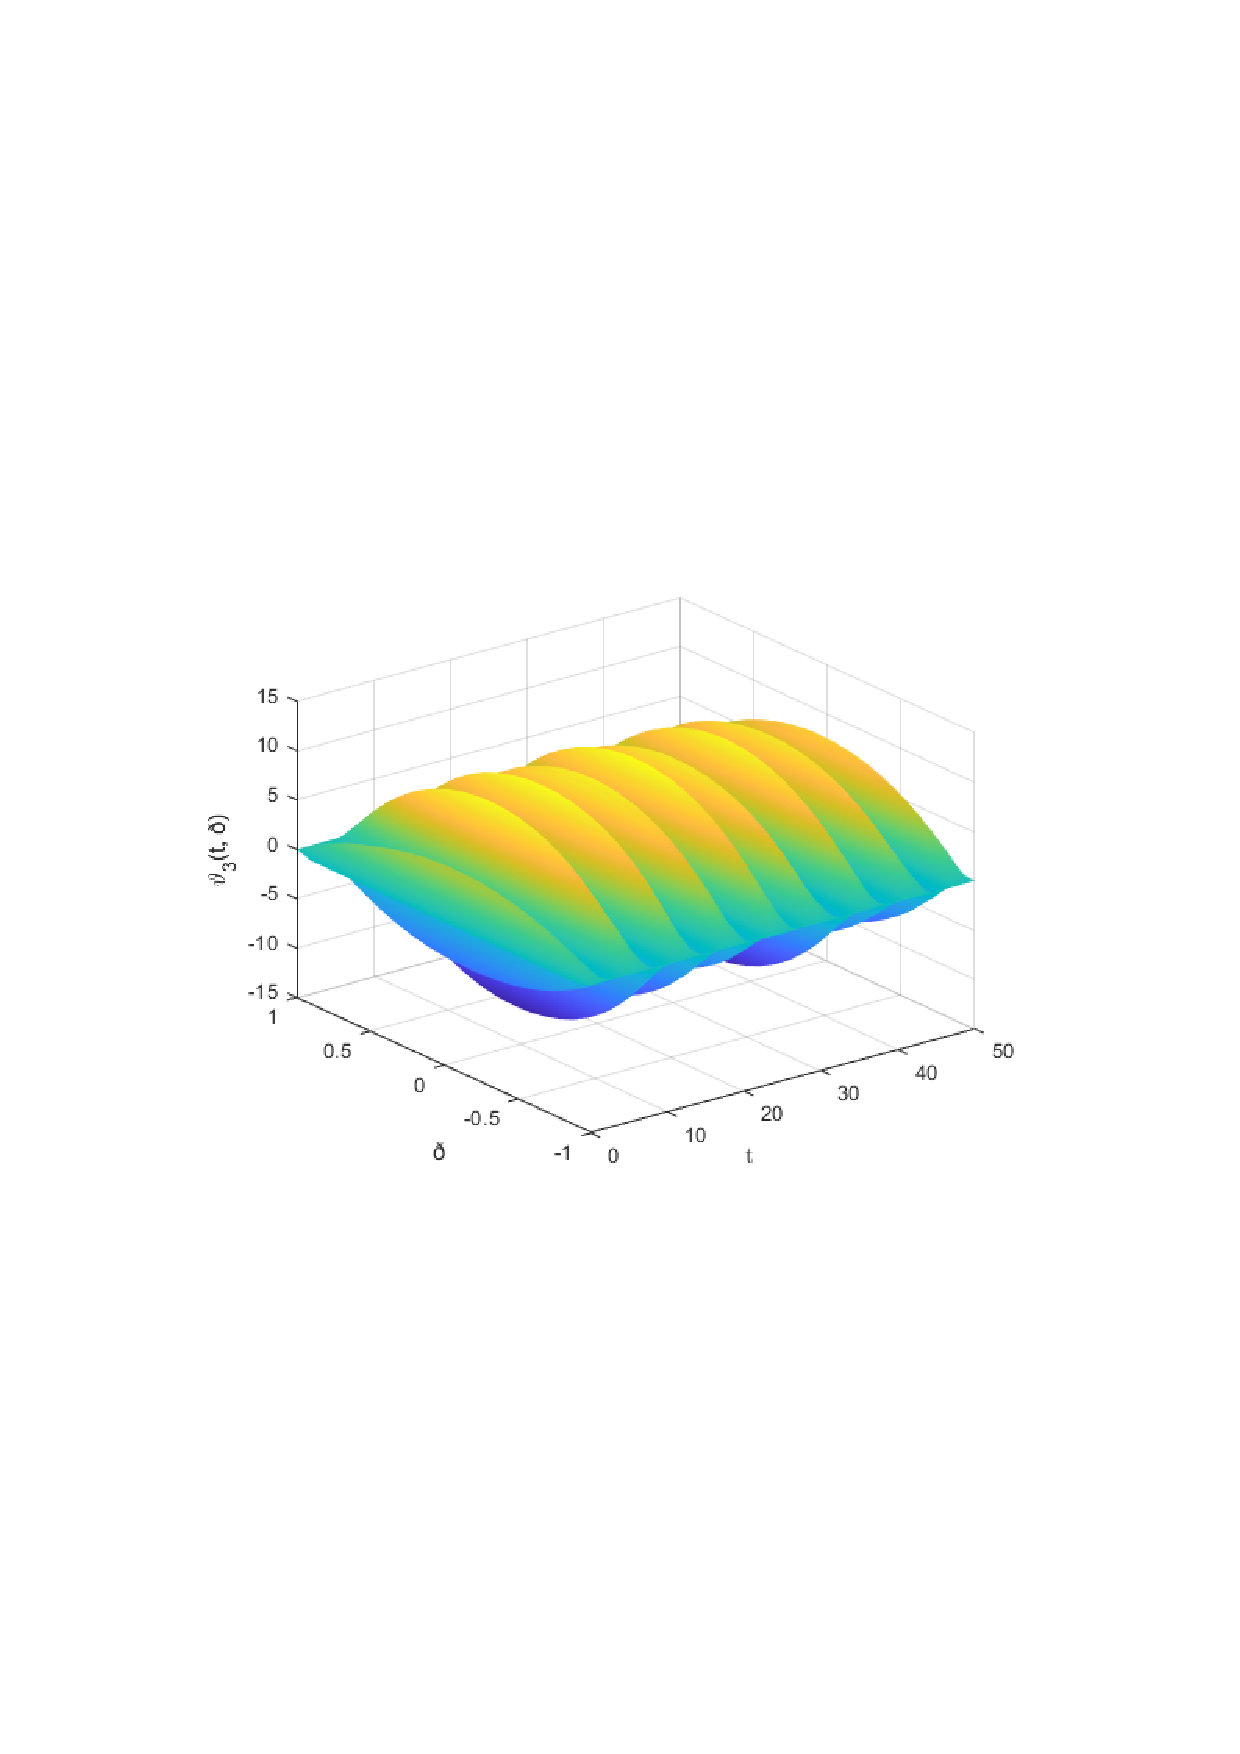
\includegraphics[width=0.45\textwidth]{figs/e3.3.pdf}}
	\caption{The open-loop error trajectories in Example \ref{example2}. (a) $\vartheta_1(t,\eth)$. (b) $\vartheta_2(t,\eth)$. (c) $\vartheta_3(t,\eth)$. }
	\label{Fig.10}
\end{figure}

Additionally, the boundary conditions are specified as Dirichlet type, and initial values are prescribed as 
\begin{align*}
	\aleph(v,\eth)&=\begin{bmatrix}
		0.5\\0.2\\-0.5
	\end{bmatrix},
	\Im(v,\eth)=\begin{bmatrix}
		-0.5\\-0.4\\-1
	\end{bmatrix},\,(v, \eth) \in [-\wp, 0] \times \Omega,
\end{align*}

All other parameters follow the definitions given in Example \ref{example1}. By solving LMIs \eqref{equ45}–\eqref{equ47}, the estimator gains are obtained:
\begin{align*}
	L_1=\begin{bmatrix}
		3.7217&-0.3059&-2.7142\\4.1468&4.2547&-6.2467\\-7.5846&-5.3806&10.2904
	\end{bmatrix},
	L_2=\begin{bmatrix}
		7.0137&-1.1142&-4.1955\\-1.3542&4.9895&-2.7397\\-2.0801&-5.1803&6.3193
	\end{bmatrix},
	L_3=\begin{bmatrix}
		4.4505&-0.7140&-3.1025\\0.3863&6.2971&-4.7725\\-4.0453&-5.3439&8.4867
	\end{bmatrix}.
\end{align*}
\begin{figure}[H]
\centering
\subfigure[]{
	\label{Fig.11.a}
	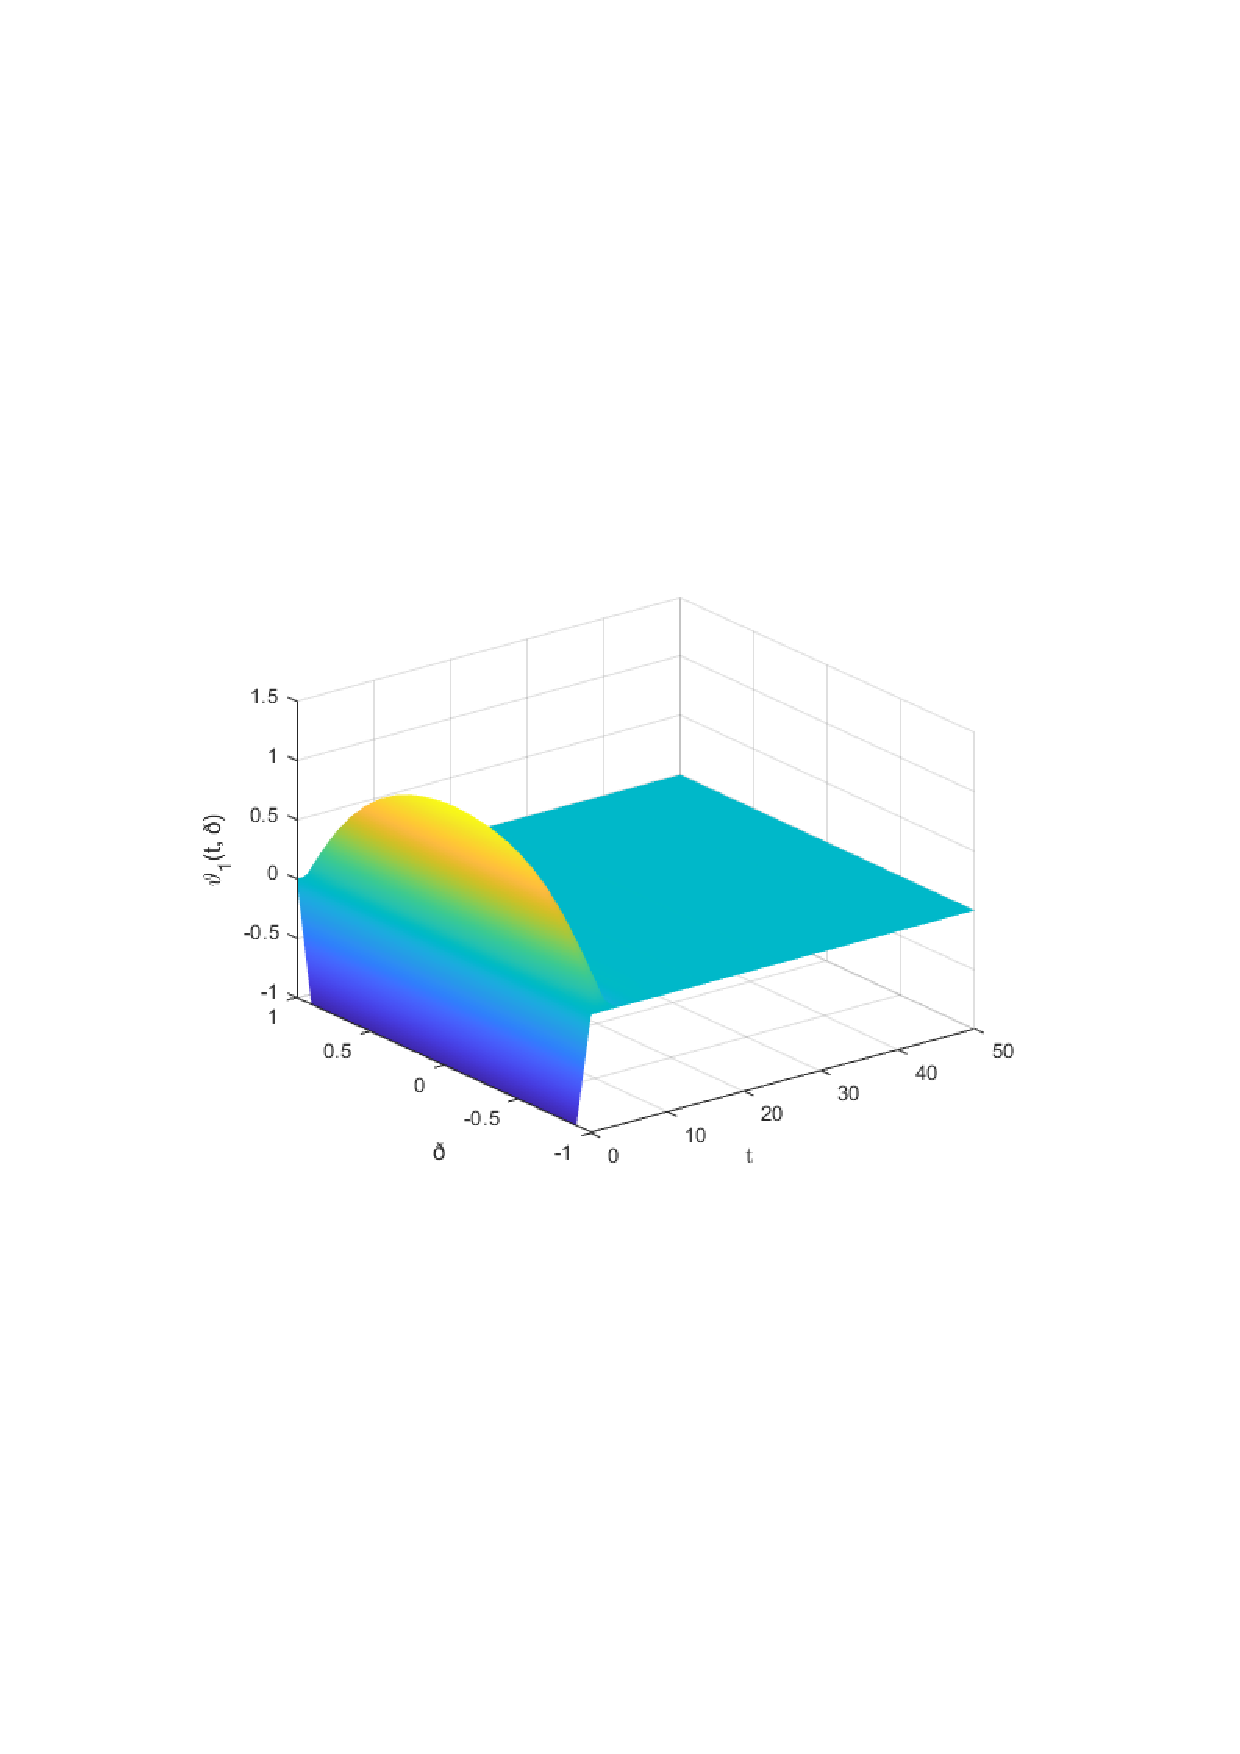
\includegraphics[width=0.45\textwidth]{figs/e1.3-e.pdf}}
\vskip\baselineskip
\subfigure[]{
	\label{Fig.11.b}
	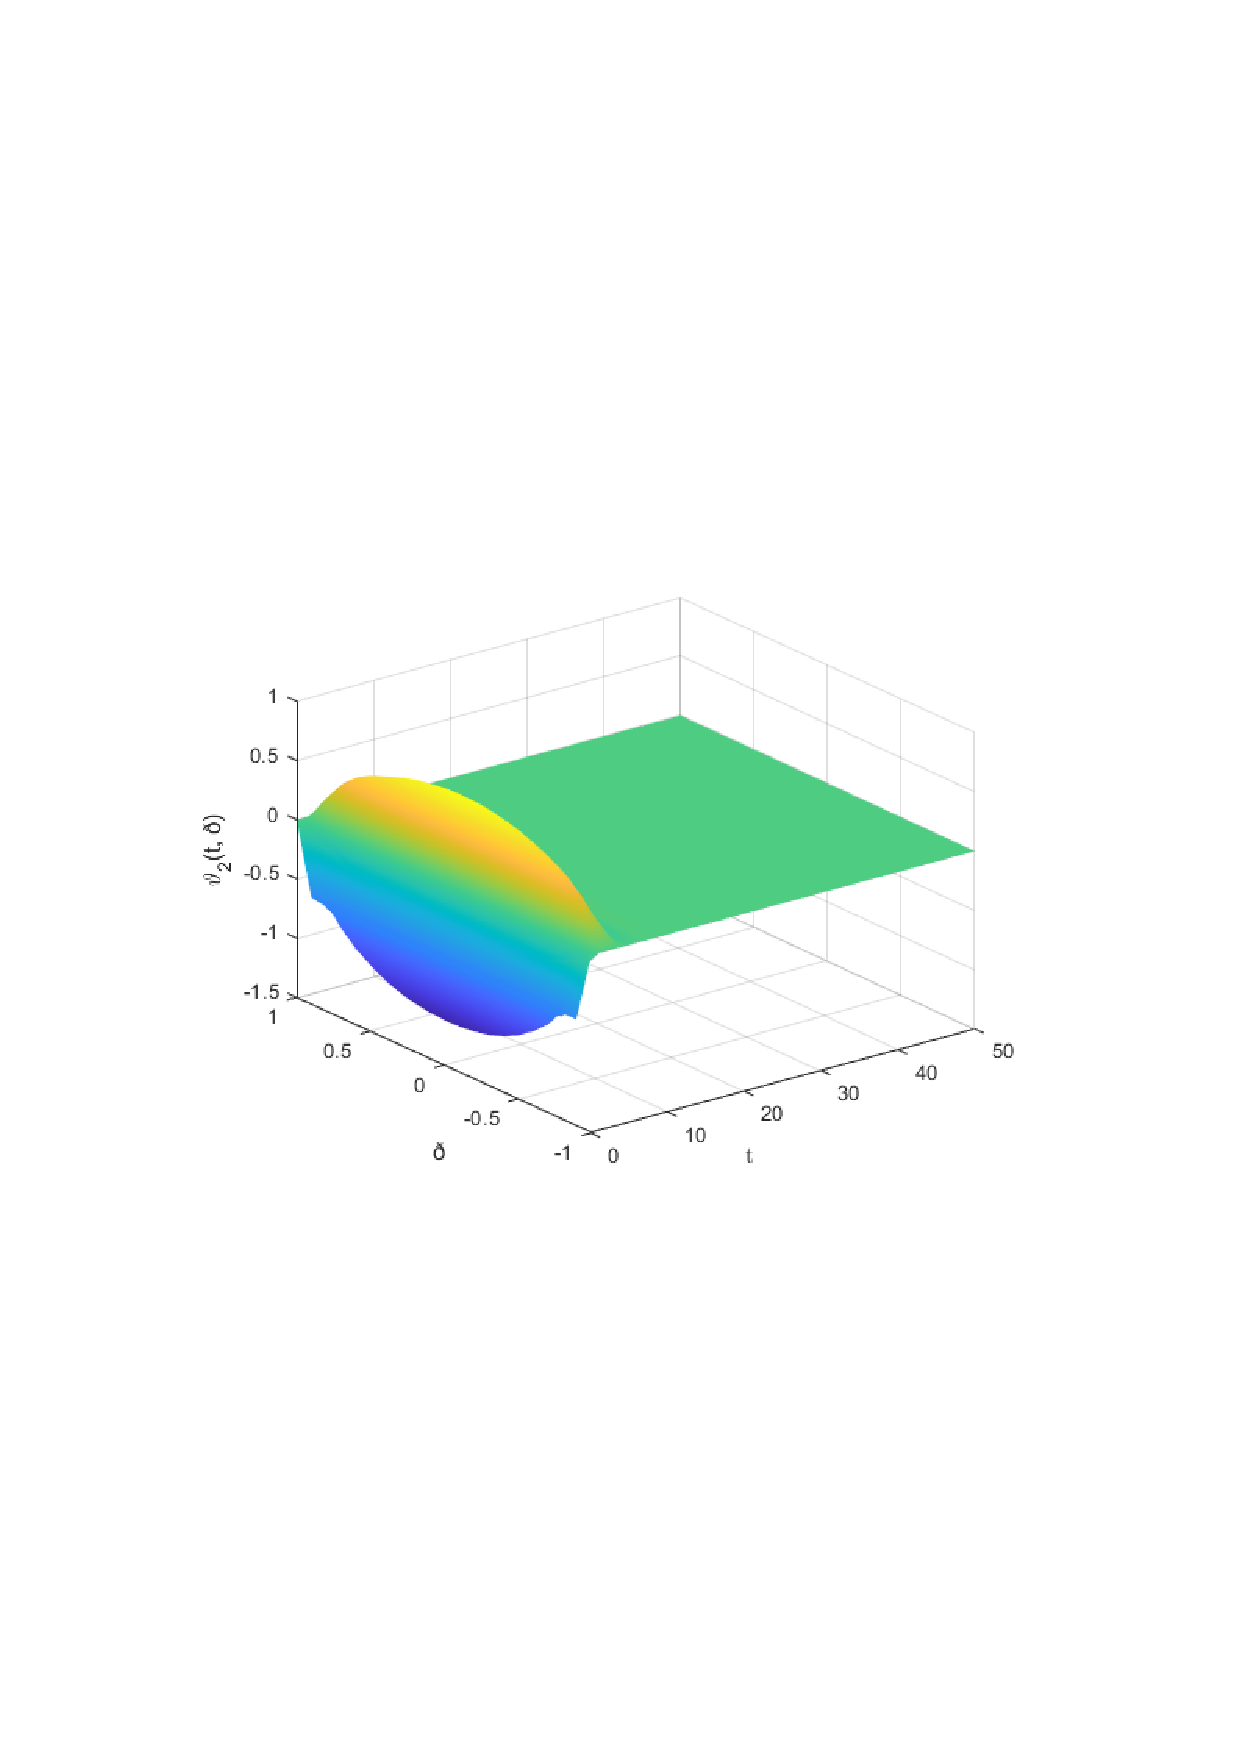
\includegraphics[width=0.45\textwidth]{figs/e2.3-e.pdf}}
\subfigure[]{
	\label{Fig.11.c}
	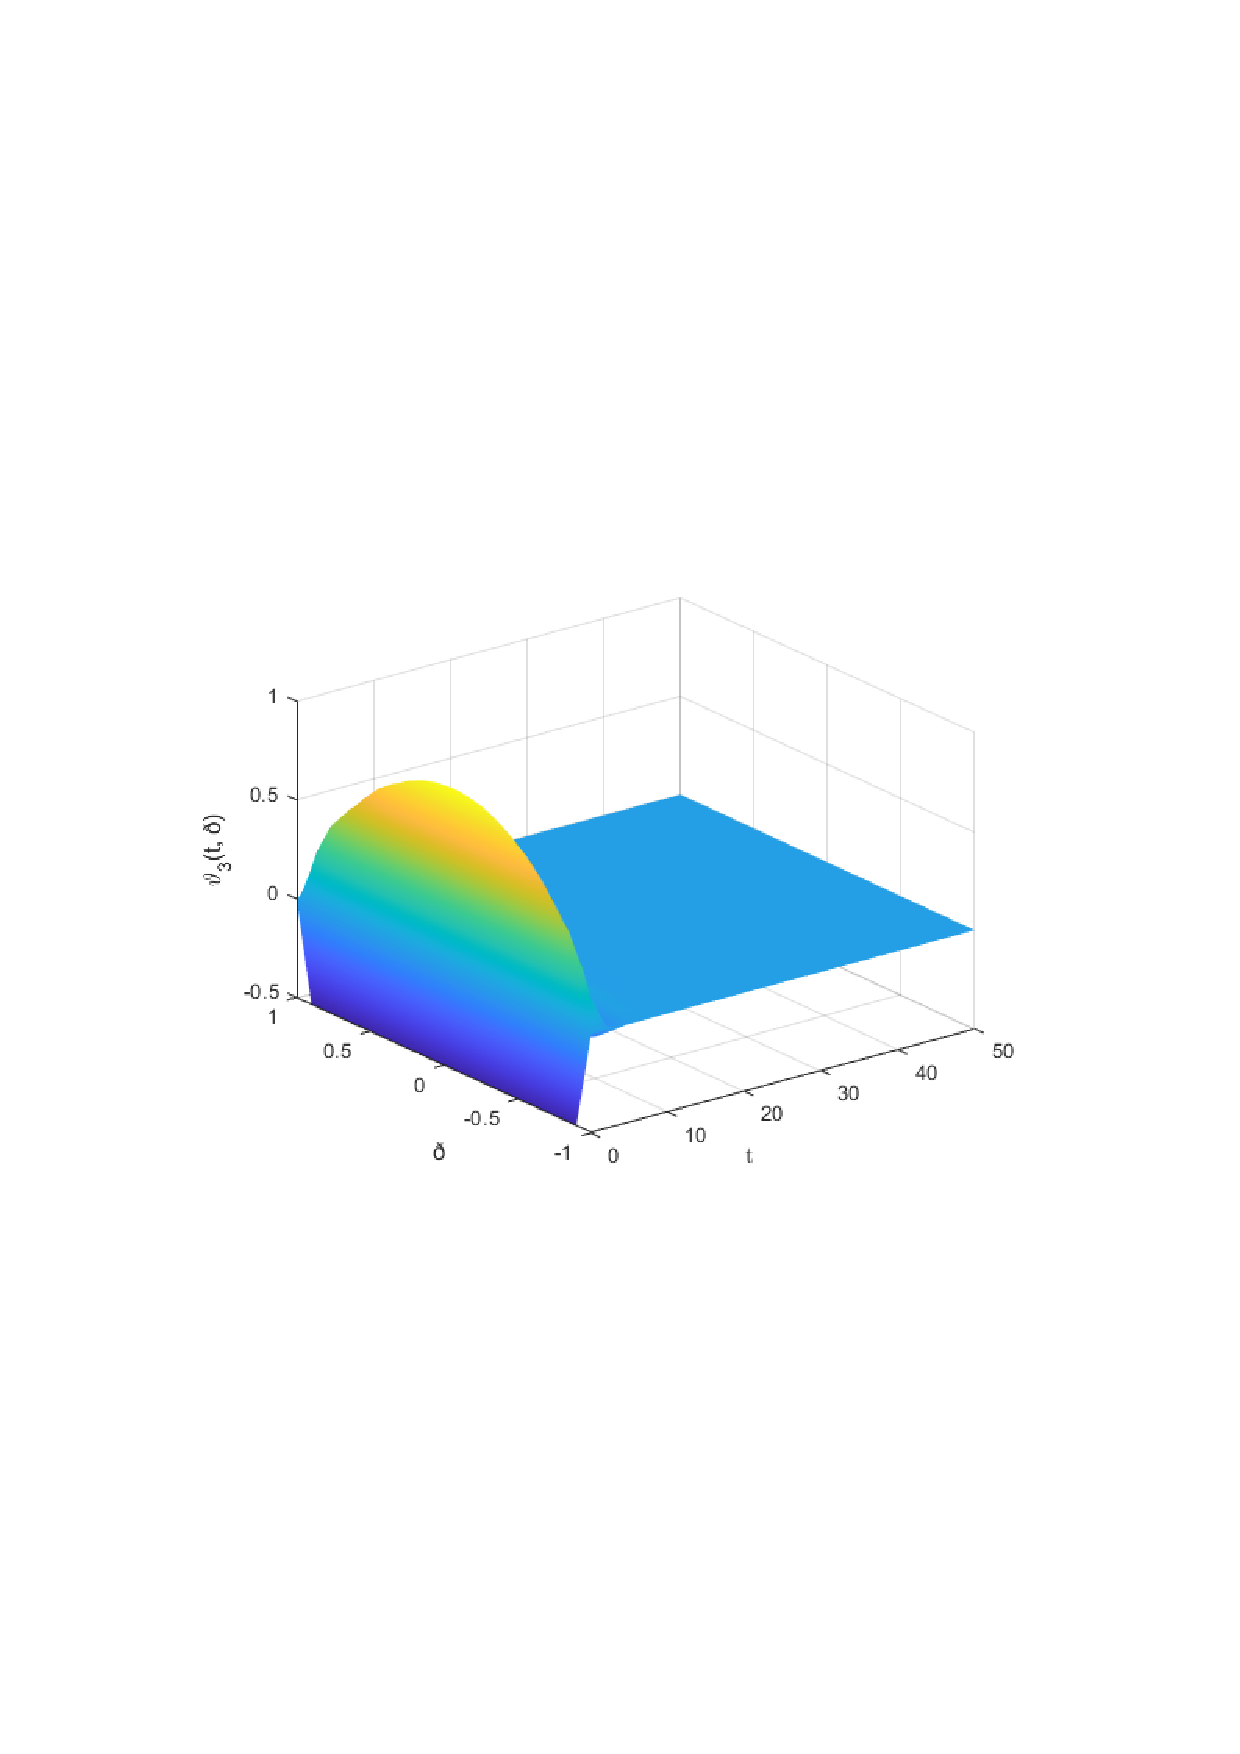
\includegraphics[width=0.45\textwidth]{figs/e3.3-e.pdf}}
\caption{The closed-loop error trajectories in Example \ref{example2}. (a) $\vartheta_1(t,\eth)$. (b) $\vartheta_2(t,\eth)$. (c) $\vartheta_3(t,\eth)$. }
\label{Fig.11}
\end{figure}

Fig.~\ref{Fig.9} illustrates the evolution of the semi-Markov switching signal across three modes. Correspondingly, Fig.~\ref{Fig.10} and Fig.~\ref{Fig.11} respectively depict the open-loop and closed-loop error trajectories. Specifically, the error trajectories at the spatial point $\eth = 0.5$ is given in Fig.~\ref{Fig.12}. Simulation results show that the ORSE provides accurate state estimation while effectively reducing outlier-induced degradation of RSE performance.
\end{example}

In conclusion, the simulation results validate the accuracy of ORSE and demonstrate its effectiveness in suppressing the interference of outliers during the RSE process.
\begin{figure}[H]
	\centering
	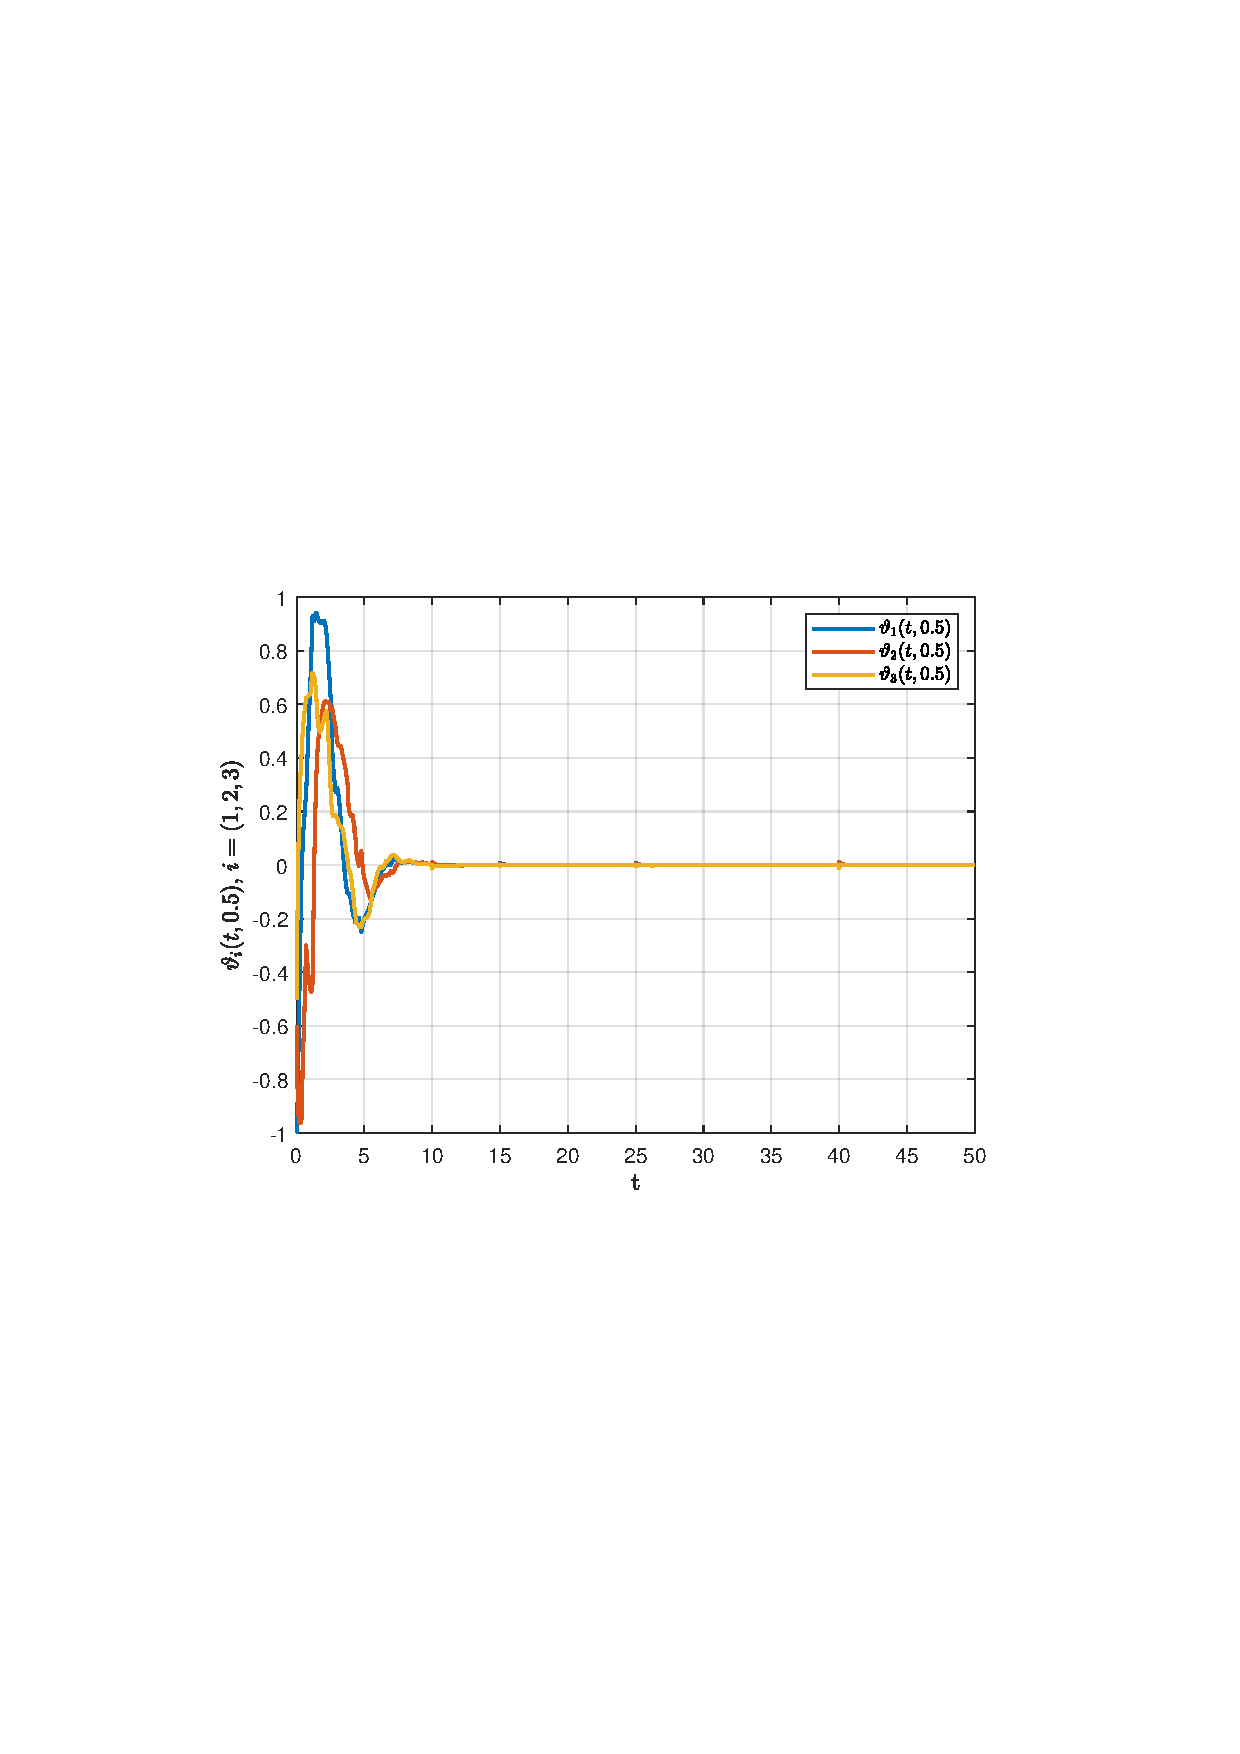
\includegraphics[width=3.5in]{figs/e1e2e3.pdf}
	\caption{The error trajectories at $\eth=0.5$ in Example \ref{example2}.}
	\label{Fig.12}
\end{figure}
\section{Conclusion} \label{sec5}
The outlier-resistant $\text{H}_\infty$ RSE problem for semi-Markov switching delayed RDNNs has been investigated in this paper. By incorporating spatial reaction-diffusion dynamics and network parameter jumps, a NNs model has been established, providing a comprehensive framework for analysis. Additionally, in consideration of probabilistic gain fluctuations and measurement outliers, an ORSE has been developed, thereby enhancing the robustness of the estimator. In addition, by constructing a mode-dependent LKF, Sufficient conditions ensuring the asymptotic stability and $\text{H}_\infty$ performance of the error system have been established. Eventually, two numerical examples are presented to verify the effectiveness of the proposed theoretical methodology. {\color{red}In the future, we will consider the case of asynchronous switching between the estimator and system modes. Additionally, to further improve the estimation performance of outlier-resistant estimator, it will be necessary to enhance the estimator structure, such as by adopting a saturation function with dynamic thresholds.}

\section*{CRediT authorship contribution statement}
{\bf Xiaoqing Li}: Conceptualization, Methodology, Writing–original draft, Writing–review \& editing. 
{\bf Xinyuan Hu}: Methodology, Writing–review \& editing. {\bf Wenjing Ren}: Conceptualization, Visualization, Writing–review \& editing. {\bf Yu Yang}: Conceptualization, Visualization, Writing–review \& editing.  {\bf Jun Cheng}: Project administration, English checking and editing. {\bf Kaibo Shi}: Conceptualization, Visualization, Writing–review \& editing.

\section*{Declaration of competing interests}
We hereby declare that this publication is free from any known conflicts of interest, and that no substantial financial support was received that might have affected the integrity or outcome of the research.

\section*{Acknowledgments}
This research was jointly supported by the National Natural Science Foundation of China under Grant (Nos. 62203147, 62203148 and 62376083).

\section*{Data availability}
Data sharing does not apply to this article, as no datasets were created or analyzed in the course of the present study.

\bibliographystyle{elsarticle-num} 
\bibliography{ref} 
\end{document}

\endinput
%%
%% End of file `elsarticle-template-num.tex'.
